%%%%%%%%%%%%%%%%%%%%%%%%%%%%%%%%%%%%%%%%%%%%%%%%%%%%%%%%%%%%%%%
%% CATTOLICA THESIS TEMPLATE

% Use this template to produce a standard thesis that meets the Oxford University requirements for either Bachelor/Master and DPhil submissions
%
% Originally by Keith A. Gillow (gillow@maths.ox.ac.uk), 1997
% Modified by Sam Evans (sam@samuelevansresearch.org), 2007
% Modified by John McManigle (john@oxfordechoes.com), 2015
% Modified by Ulrik Lyngs (ulrik.lyngs@cs.ox.ac.uk), 2018-, for use with R Markdown
% Modified by Niccolo Salvini  (niccolo.salvini01@unicatt.it), 2022, for use with R Markdown in UCSC
%
% Ulrik Lyngs, 25 Nov 2018: Following John McManigle, broad permissions are granted to use, modify, and distribute this software
% as specified in the MIT License included in this distribution's LICENSE file.
%
% John commented this file extensively, so read through to see how to use the various options.  Remember that in LaTeX,
% any line starting with a % is NOT executed.  Several places below, you have a choice of which line to use
% out of multiple options (eg draft vs final, for PDF vs for binding, etc.)  When you pick one, add a % to the beginning of
% the lines you don't want.


%%%%% PAGE LAYOUT
% The most common choices should be below.  You can also do other things, like replacing "a4paper" with "letterpaper", etc.

% This one formats for two-sided binding (ie left and right pages have mirror margins; blank pages inserted where needed):
%\documentclass[a4paper,twoside]{templates/ociamthesis}
% This one formats for one-sided binding (ie left margin > right margin; no extra blank pages):
%\documentclass[a4paper]{templates/ociamthesis}
% This one formats for PDF output (ie equal margins, no extra blank pages):
%\documentclass[a4paper,nobind]{templates/ociamthesis}

% As you can see from the uncommented line below, oxforddown template uses the a4paper size, 
% and passes in the binding option from the YAML header in index.Rmd:
% altered 11pt
\documentclass[a4paper, 11pt, nobind]{templates/ociamthesis}


%%%%% ADDING LATEX PACKAGES
% add hyperref package with options from YAML %
\usepackage[pdfpagelabels]{hyperref}
% handle long urls
\usepackage{xurl}
% change the default coloring of links to something sensible
\usepackage{xcolor}

\definecolor{mylinkcolor}{RGB}{0,0,139}
\definecolor{myurlcolor}{RGB}{0,0,139}
\definecolor{mycitecolor}{RGB}{0,33,71}

\hypersetup{
  hidelinks,
  colorlinks,
  linktocpage=true,
  linkcolor=mylinkcolor,
  urlcolor=myurlcolor,
  citecolor=mycitecolor
}



% add float package to allow manual control of figure positioning %
\usepackage{float}

% enable strikethrough
\usepackage[normalem]{ulem}

% use soul package for correction highlighting
\usepackage{color, soulutf8}
\definecolor{correctioncolor}{HTML}{CCCCFF}
\sethlcolor{correctioncolor}
\newcommand{\ctext}[3][RGB]{%
  \begingroup
  \definecolor{hlcolor}{#1}{#2}\sethlcolor{hlcolor}%
  \hl{#3}%
  \endgroup
}
\soulregister\ref7
\soulregister\cite7
\soulregister\citet7
\soulregister\autocite7
\soulregister\textcite7
\soulregister\pageref7

%%%%% FIXING / ADDING THINGS THAT'S SPECIAL TO R MARKDOWN'S USE OF LATEX TEMPLATES
% pandoc puts lists in 'tightlist' command when no space between bullet points in Rmd file,
% so we add this command to the template
\providecommand{\tightlist}{%
  \setlength{\itemsep}{0pt}\setlength{\parskip}{0pt}}
 
% UL 1 Dec 2018, fix to include code in shaded environments
\usepackage{color}
\usepackage{fancyvrb}
\newcommand{\VerbBar}{|}
\newcommand{\VERB}{\Verb[commandchars=\\\{\}]}
\DefineVerbatimEnvironment{Highlighting}{Verbatim}{commandchars=\\\{\}}
% Add ',fontsize=\small' for more characters per line
\usepackage{framed}
\definecolor{shadecolor}{RGB}{248,248,248}
\newenvironment{Shaded}{\begin{snugshade}}{\end{snugshade}}
\newcommand{\AlertTok}[1]{\textcolor[rgb]{0.94,0.16,0.16}{#1}}
\newcommand{\AnnotationTok}[1]{\textcolor[rgb]{0.56,0.35,0.01}{\textbf{\textit{#1}}}}
\newcommand{\AttributeTok}[1]{\textcolor[rgb]{0.77,0.63,0.00}{#1}}
\newcommand{\BaseNTok}[1]{\textcolor[rgb]{0.00,0.00,0.81}{#1}}
\newcommand{\BuiltInTok}[1]{#1}
\newcommand{\CharTok}[1]{\textcolor[rgb]{0.31,0.60,0.02}{#1}}
\newcommand{\CommentTok}[1]{\textcolor[rgb]{0.56,0.35,0.01}{\textit{#1}}}
\newcommand{\CommentVarTok}[1]{\textcolor[rgb]{0.56,0.35,0.01}{\textbf{\textit{#1}}}}
\newcommand{\ConstantTok}[1]{\textcolor[rgb]{0.00,0.00,0.00}{#1}}
\newcommand{\ControlFlowTok}[1]{\textcolor[rgb]{0.13,0.29,0.53}{\textbf{#1}}}
\newcommand{\DataTypeTok}[1]{\textcolor[rgb]{0.13,0.29,0.53}{#1}}
\newcommand{\DecValTok}[1]{\textcolor[rgb]{0.00,0.00,0.81}{#1}}
\newcommand{\DocumentationTok}[1]{\textcolor[rgb]{0.56,0.35,0.01}{\textbf{\textit{#1}}}}
\newcommand{\ErrorTok}[1]{\textcolor[rgb]{0.64,0.00,0.00}{\textbf{#1}}}
\newcommand{\ExtensionTok}[1]{#1}
\newcommand{\FloatTok}[1]{\textcolor[rgb]{0.00,0.00,0.81}{#1}}
\newcommand{\FunctionTok}[1]{\textcolor[rgb]{0.00,0.00,0.00}{#1}}
\newcommand{\ImportTok}[1]{#1}
\newcommand{\InformationTok}[1]{\textcolor[rgb]{0.56,0.35,0.01}{\textbf{\textit{#1}}}}
\newcommand{\KeywordTok}[1]{\textcolor[rgb]{0.13,0.29,0.53}{\textbf{#1}}}
\newcommand{\NormalTok}[1]{#1}
\newcommand{\OperatorTok}[1]{\textcolor[rgb]{0.81,0.36,0.00}{\textbf{#1}}}
\newcommand{\OtherTok}[1]{\textcolor[rgb]{0.56,0.35,0.01}{#1}}
\newcommand{\PreprocessorTok}[1]{\textcolor[rgb]{0.56,0.35,0.01}{\textit{#1}}}
\newcommand{\RegionMarkerTok}[1]{#1}
\newcommand{\SpecialCharTok}[1]{\textcolor[rgb]{0.00,0.00,0.00}{#1}}
\newcommand{\SpecialStringTok}[1]{\textcolor[rgb]{0.31,0.60,0.02}{#1}}
\newcommand{\StringTok}[1]{\textcolor[rgb]{0.31,0.60,0.02}{#1}}
\newcommand{\VariableTok}[1]{\textcolor[rgb]{0.00,0.00,0.00}{#1}}
\newcommand{\VerbatimStringTok}[1]{\textcolor[rgb]{0.31,0.60,0.02}{#1}}
\newcommand{\WarningTok}[1]{\textcolor[rgb]{0.56,0.35,0.01}{\textbf{\textit{#1}}}}

%UL set white space before and after code blocks
\renewenvironment{Shaded}
{
  \vspace{10pt}%
  \begin{snugshade}%
}{%
  \end{snugshade}%
  \vspace{8pt}%
}

% User-included things with header_includes or in_header will appear here
% kableExtra packages will appear here if you use library(kableExtra)
\usepackage{booktabs}
\usepackage{longtable}
\usepackage{array}
\usepackage{multirow}
\usepackage{wrapfig}
\usepackage{float}
\usepackage{colortbl}
\usepackage{pdflscape}
\usepackage{tabu}
\usepackage{threeparttable}
\usepackage{threeparttablex}
\usepackage[normalem]{ulem}
\usepackage{makecell}
\usepackage{xcolor}


%UL set section header spacing
\usepackage{titlesec}
% 
\titlespacing\subsubsection{0pt}{24pt plus 4pt minus 2pt}{0pt plus 2pt minus 2pt}


%UL set whitespace around verbatim environments
\usepackage{etoolbox}
\makeatletter
\preto{\@verbatim}{\topsep=0pt \partopsep=0pt }
\makeatother


%%%%%%% PAGE HEADERS AND FOOTERS %%%%%%%%%
\usepackage{fancyhdr}
\setlength{\headheight}{15pt}
\fancyhf{} % clear the header and footers
\pagestyle{fancy}
\renewcommand{\chaptermark}[1]{\markboth{\thechapter. #1}{\thechapter. #1}}
\renewcommand{\sectionmark}[1]{\markright{\thesection. #1}} 
\renewcommand{\headrulewidth}{0pt}

\fancyhead[LO]{\emph{\leftmark}} 
\fancyhead[RE]{\emph{\rightmark}} 

% UL page number position 
\fancyfoot[C]{\emph{\thepage}} %regular pages
\fancypagestyle{plain}{\fancyhf{}\fancyfoot[C]{\emph{\thepage}}} %chapter pages


%%%%% SELECT YOUR DRAFT OPTIONS
% This adds a "DRAFT" footer to every normal page.  (The first page of each chapter is not a "normal" page.)

% IP feb 2021: option to include line numbers in PDF

% for line wrapping in code blocks
\usepackage{fancyvrb}
\usepackage{fvextra}
\DefineVerbatimEnvironment{Highlighting}{Verbatim}{breaklines=true, breakanywhere=true, commandchars=\\\{\}}

% This highlights (in blue) corrections marked with (for words) \mccorrect{blah} or (for whole
% paragraphs) \begin{mccorrection} . . . \end{mccorrection}.  This can be useful for sending a PDF of
% your corrected thesis to your examiners for review.  Turn it off, and the blue disappears.
\correctionstrue


%%%%% BIBLIOGRAPHY SETUP
% Note that your bibliography will require some tweaking depending on your department, preferred format, etc.
% If you've not used LaTeX before, I recommend reading a little about biblatex/biber and getting started with it.
% If you're already a LaTeX pro and are used to natbib or something, modify as necessary.
% Either way, you'll have to choose and configure an appropriate bibliography format...

% this enables pandoc citations
\newlength{\cslhangindent}
\setlength{\cslhangindent}{1.5em}
\newlength{\csllabelwidth}
\setlength{\csllabelwidth}{3em}
\newlength{\cslentryspacingunit} % times entry-spacing
\setlength{\cslentryspacingunit}{\parskip}
\newenvironment{CSLReferences}[2] % #1 hanging-ident, #2 entry spacing
 {% don't indent paragraphs
  \setlength{\parindent}{0pt}
  % turn on hanging indent if param 1 is 1
  \ifodd #1
  \let\oldpar\par
  \def\par{\hangindent=\cslhangindent\oldpar}
  \fi
  % set entry spacing
  \setlength{\parskip}{1mm}
  \setlength{\baselineskip}{6mm}
 }%
 {}
\usepackage{calc}
\newcommand{\CSLBlock}[1]{#1\hfill\break}
\newcommand{\CSLLeftMargin}[1]{\parbox[t]{\csllabelwidth}{#1}}
\newcommand{\CSLRightInline}[1]{\parbox[t]{\linewidth - \csllabelwidth}{#1}\break}
\newcommand{\CSLIndent}[1]{\hspace{\cslhangindent}#1}




% Uncomment this if you want equation numbers per section (2.3.12), instead of per chapter (2.18):
%\numberwithin{equation}{subsection}


%%%%% THESIS / TITLE PAGE INFORMATION
% Everybody needs to complete the following:
\title{\texttt{cattolicadown}:\\
An UCSC Thesis\\
Template for R Markdown}
\author{Author Name}
\college{Your College}

% Master's candidates who require the alternate title page (with candidate number and word count)
% must also un-comment and complete the following three lines:

% Uncomment the following line if your degree also includes exams (eg most masters):
%\renewcommand{\submittedtext}{Submitted in partial completion of the}
% Your full degree name.  (But remember that DPhils aren't "in" anything.  They're just DPhils.)
\degree{MSc in}
% Term and year of submission, or date if your board requires (eg most masters)
\degreedate{5th July 2023}


%%%%% YOUR OWN PERSONAL MACROS
% This is a good place to dump your own LaTeX macros as they come up.

% To make text superscripts shortcuts
	\renewcommand{\th}{\textsuperscript{th}} % ex: I won 4\th place
	\newcommand{\nd}{\textsuperscript{nd}}
	\renewcommand{\st}{\textsuperscript{st}}
	\newcommand{\rd}{\textsuperscript{rd}}

%%%%% THE ACTUAL DOCUMENT STARTS HERE
\begin{document}

%%%%% CHOOSE YOUR LINE SPACING HERE
% This is the official option.  Use it for your submission copy and library copy:
\setlength{\textbaselineskip}{22pt plus2pt}
% This is closer spacing (about 1.5-spaced) that you might prefer for your personal copies:
%\setlength{\textbaselineskip}{18pt plus2pt minus1pt}

% You can set the spacing here for the roman-numbered pages (acknowledgements, table of contents, etc.)
\setlength{\frontmatterbaselineskip}{17pt plus1pt minus1pt}

% UL: You can set the line and paragraph spacing here for the separate abstract page to be handed in to Examination schools
\setlength{\abstractseparatelineskip}{13pt plus1pt minus1pt}
\setlength{\abstractseparateparskip}{0pt plus 1pt}

% UL: You can set the general paragraph spacing here - I've set it to 2pt (was 0) so
% it's less claustrophobic
\setlength{\parskip}{2pt plus 1pt}

%
% Customise title page
%
\def\crest{{
\includegraphics[width=5cm]{templates/cattolica-logo.pdf}}}
\renewcommand{\university}{Catholic University of Sacred Heart (, sede)}
\renewcommand{\submittedtext}{A thesis submitted for the degree of}
\renewcommand{\thesistitlesize}{\fontsize{22pt}{28pt}\selectfont}
\renewcommand{\gapbeforecrest}{25mm}
\renewcommand{\gapaftercrest}{25mm}


% Leave this line alone; it gets things started for the real document.
\setlength{\baselineskip}{\textbaselineskip}


%%%%% CHOOSE YOUR SECTION NUMBERING DEPTH HERE
% You have two choices.  First, how far down are sections numbered?  (Below that, they're named but
% don't get numbers.)  Second, what level of section appears in the table of contents?  These don't have
% to match: you can have numbered sections that don't show up in the ToC, or unnumbered sections that
% do.  Throughout, 0 = chapter; 1 = section; 2 = subsection; 3 = subsubsection, 4 = paragraph...

% The level that gets a number:
\setcounter{secnumdepth}{2}
% The level that shows up in the ToC:
\setcounter{tocdepth}{1}


%%%%% ABSTRACT SEPARATE
% This is used to create the separate, one-page abstract that you are required to hand into the Exam
% Schools.  You can comment it out to generate a PDF for printing or whatnot.

% JEM: Pages are roman numbered from here, though page numbers are invisible until ToC.  This is in
% keeping with most typesetting conventions.
\begin{romanpages}

% Title page is created here
\maketitle

%%%%% DEDICATION
\begin{dedication}
  For my Mum
\end{dedication}

%%%%% ACKNOWLEDGEMENTS


\begin{acknowledgements}
 	È qui che normalmente ringrazierai il tuo relator* /correlator\emph{, collegh}, la famiglia e gli amici, nonché i finanziamenti e il supporto istituzionale. Nel nostro caso, daremo le tesseremo le lodi alle persone che hanno sviluppato le idee e gli strumenti che ci consentono di spingere la scienza aperta un piccolo passo avanti scrivendo tesi trasparenti e riproducibili in R Markdown.

 Dobbiamo essere grati a John Gruber per aver inventato la versione originale di Markdown, a John MacFarlane per aver creato Pandoc (\url{http://pandoc.org}) che converte Markdown in un gran numero di formati di output e a Yihui Xie per aver creato \texttt{knitr} che ha introdotto R Markdown come un modo per incorporare il codice nei documenti Markdown e \texttt{bookdown} che ha aggiunto strumenti per la scrittura tecnica in forma più estesa.

 Un ringraziamento speciale a \href{http://chester.rbind.io}{Chester Ismay}, che ha creato il pacchetto \texttt{thesisdown} che ha aiutato molti dottorandi a scrivere le loro tesi in R Markdown.

 Infine, un profondo ringraziamento a JJ Allaire, fondatore e CEO di \href{http://rstudio.com}{RStudio}, e Hadley Wickham, la mente del tidyverse senza il quale ci saremmo semplicemente arresi e avremmo fatto scienza dei dati in Python, sbagliando. Grazie per aver reso la scienza dei dati più semplice, più accessibile e più divertente per tutti noi.

 \begin{flushright}
 Niccolo Salvini \\
 Campus Gemelli, Roma \\
 5 Luglio 2022
 \end{flushright}
\end{acknowledgements}



%%%%% ABSTRACT


\renewcommand{\abstracttitle}{Abstract}
\begin{abstract}
	Questo template \emph{R Markdown} serve per scrivere una tesi dell'Università Cattolica del Sacro Cuore di tutte le sedi, di tutti i corsi di laurea.
Il template è costruito usando il pacchetto \texttt{bookdown} di Yihui Xie, con una forte ispirazione da \texttt{thesisdown} di Chester Ismay e dal template \texttt{OxThesis} \LaTeX~(più recentemente riadattato da John McManigle).

Il contenuto di esempio di questo template include illustrazioni su come scrivere una tesi in R Markdown e segue in gran parte la struttura di \href{https://ulyngs.github.io/rmarkdown-workshop-2019/}{questo workshop R Markdown} a cura di un ricercatore dell'università di Oxford, da cui ho presto molta ispirazione.

Congratulazioni per aver fatto un ulteriore passo avanti nelle terre della scienza open e riproducibile utilizzando uno strumento sottovalutato che ti consente di includere in modo trasparente tabelle e grafici generati direttamente dai dati sottostanti.
\end{abstract}



%%%%% MINI TABLES
% This lays the groundwork for per-chapter, mini tables of contents.  Comment the following line
% (and remove \minitoc from the chapter files) if you don't want this.  Un-comment either of the
% next two lines if you want a per-chapter list of figures or tables.
  \dominitoc % include a mini table of contents

% This aligns the bottom of the text of each page.  It generally makes things look better.
\flushbottom

% This is where the whole-document ToC appears:
\tableofcontents

\listoffigures
	\mtcaddchapter
  	% \mtcaddchapter is needed when adding a non-chapter (but chapter-like) entity to avoid confusing minitoc

% Uncomment to generate a list of tables:
\listoftables
  \mtcaddchapter
%%%%% LIST OF ABBREVIATIONS
% This example includes a list of abbreviations.  Look at text/abbreviations.tex to see how that file is
% formatted.  The template can handle any kind of list though, so this might be a good place for a
% glossary, etc.
% First parameter can be changed eg to "Glossary" or something.
% Second parameter is the max length of bold terms.
\begin{mclistof}{List of Abbreviations}{3.2cm}

\item[1-D, 2-D]

Mono o bidimensionale, riferendosi \textbf{in questa tesi} alle dimensioni spaziali di un'immagine.

\item[Lontra]

Uno dei mammiferi acquatici più belli.

\item[Riccio]

Davvero un simpatico amico spinoso.

\end{mclistof} 


% The Roman pages, like the Roman Empire, must come to its inevitable close.
\end{romanpages}

%%%%% CHAPTERS
% Add or remove any chapters you'd like here, by file name (excluding '.tex'):
\flushbottom

% all your chapters and appendices will appear here
\hypertarget{introduzione}{%
\chapter*{Introduzione}\label{introduzione}}
\addcontentsline{toc}{chapter}{Introduzione}

\adjustmtc
\markboth{Introduction}{}

Benvenuto in \texttt{cattolicadown} (\protect\hyperlink{ref-lyngscattolicadown2019}{\textbf{lyngscattolicadown2019?}}), un template di tesi per R Markdown che ho creato per i laureandi dell'Università Cattolica del Sacro Cuore (per tutte le sedi, per tutte le lauree).
Questo template ti consente di scrivere tutta la tesi in R Markdown, mentre formatti l'.output PDF con il bellissimo e collaudato \href{https://github.com/mcmanigle/OxThesis}{OxThesis LaTeX template}.
Questo è un contributo, in parte adattato ed open source che si ispira a \href{https://github.com/ismayc/thesisdown}{\texttt{thesisdown}}.

Si spera che scrivere la tua tesi in R Markdown fornisca un'interfaccia migliore per latex (OxThesis se non hai mai usato TeX o LaTeX) togliendoti l'impiccio di impararlo da capo.
Ancora più importante, \emph{R Markdown} ti consente di incorporare blocchi di codice all'interno della tua tesi e generare grafici e tabelle direttamente dai dati sottostanti, evitando passaggi di copia e incolla.
Questo ti fa prendere l'abitudine di fare ricerche riproducibili, il che ti beneficerà a lungo termine come ricercatore o analista, e aiuterà anche chiunque stia cercando di riprodurre o sviluppare i tuoi risultati.

\hypertarget{perchuxe9-usarlo}{%
\section*{Perché usarlo?}\label{perchuxe9-usarlo}}
\addcontentsline{toc}{section}{Perché usarlo?}

\emph{R Markdown} crea un modo semplice e diretto per interfacciarsi con la bellezza di LaTeX.
I pacchetti sono stati scritti in \textbf{R} per lavorare direttamente con LaTeX per produrre tabelle e paragrafi ben formattati.
Oltre a creare un'interfaccia intuitiva per LaTeX, \emph{R Markdown} ti consente di leggere i tuoi dati, analizzarli e visualizzarli usando \textbf{R}, \textbf{Python} o altri linguaggi e fornire documentazione e commenti sui risultati del tuo progetto.\\
Inoltre, consente di passare i risultati dell'output del codice in linea al commento dei risultati.
Vedrai di più su questo più avanti, concentrandoti su \textbf{R}.
Se ti piace di più \textbf{Python} o qualcos'altro, puoi comunque usare \emph{R Markdown} - vedi \href{https://bookdown.org/yihui/rmarkdown/language-engines.html}{`Other language engine'} in {[}\emph{R Markdown: The Definitive Guide}{]} di Yihui Xie (\url{https://bookdown.org/yihui/rmarkdown/language-engines.html}).

L'uso di LaTeX insieme a \emph{Markdown} è più coerente dell'output di un qualsiasi altro text editor, molto meno soggetto a danneggiamento o arresto anomalo e il file risultante è più piccolo di un file di Word.
Anche se potresti non aver mai avuto problemi con Word in passato, è probabile che la tua tesi sarà circa due volte più grande e complessa di qualsiasi cosa tu abbia scritto prima, mettendo a dura prova le capacità di Word.

\hypertarget{chi-lo-dovrebbe-usare}{%
\section*{Chi lo dovrebbe usare?}\label{chi-lo-dovrebbe-usare}}
\addcontentsline{toc}{section}{Chi lo dovrebbe usare?}

Chiunque abbia bisogno di utilizzare l'analisi dei dati, la matematica, le tabelle, molte cifre, riferimenti incrociati complessi o che si preoccupa solo della riproducibilità nella ricerca può trarre vantaggio dall'utilizzo di \emph{R Markdown}.
Se stai lavorando in campi ``più morbidi'', la natura user-friendly della sintassi \emph{Markdown} e la sua capacità di tenere traccia e includere facilmente le figure, generano automaticamente un sommario, indice, riferimenti, sommario, ecc. dovrebbe comunque renderlo di grande beneficio per il tuo progetto di tesi.

Inoltre se deciderai di ospitare i files della tua tesi tramite \emph{git} in una cartella \emph{Github}, offrirai al tu* relatore/correlat* la possiblità di farti fare una PR (pull request) sul codice che genera sia il testo, sia le analisi, sia la formattazione. Questo permetterà ad entrambe di tenere traccia dei cambiamenti, dello sviluppo e limitare l'antipatia del ping-pong delle versioni, come ``final.docx'', ``final-final.docx'' e ``davvero-ultimo-final.docx''

\hypertarget{come-si-usa}{%
\chapter{Come si usa?}\label{come-si-usa}}

\minitoc 

\hypertarget{qual-uxe8-la-struttura-di-cattolicadown}{%
\section{\texorpdfstring{Qual è la struttura di \texttt{cattolicadown}}{Qual è la struttura di cattolicadown}}\label{qual-uxe8-la-struttura-di-cattolicadown}}

\begin{Shaded}
\begin{Highlighting}[]
\NormalTok{.}
\NormalTok{+{-}{-} index.Rmd}
\NormalTok{+{-}{-} \_bookdown.yml}
\NormalTok{+{-}{-} 00{-}introduction.Rmd}
\NormalTok{|   ...}
\NormalTok{+{-}{-} 07{-}conclusion.Rmd}
\NormalTok{+{-}{-} front{-}and{-}back{-}matter}
\NormalTok{|   +{-}{-} \_abstract.Rmd}
\NormalTok{|   +{-}{-} 98{-}appendices.Rmd}
\NormalTok{|   ...}
\NormalTok{+{-}{-} bibliography}
\NormalTok{|   +{-}{-} references.bib}
\NormalTok{|   ...}
\NormalTok{+{-}{-} figures}
\NormalTok{|   ...}
\NormalTok{+{-}{-} docs}
\NormalTok{|   +{-}{-} \_main.pdf}
\NormalTok{|   ...}
\NormalTok{+{-}{-} scripts\_and\_filters}
\NormalTok{|   +{-}{-} knit{-}functions.R}
\NormalTok{|   ...}
\NormalTok{+{-}{-} templates}
\NormalTok{|   +{-}{-} template.tex}
\NormalTok{|   ...}
\end{Highlighting}
\end{Shaded}

\hypertarget{index.rmd-opzioni-di-metadata-e-layout}{%
\subsection{\texorpdfstring{index.Rmd: \textbf{opzioni di metadata e layout}}{index.Rmd: opzioni di metadata e layout}}\label{index.rmd-opzioni-di-metadata-e-layout}}

In index.Rmd setti i la configurazione della tesi e.g., titolo, nome dell'autore

\begin{Shaded}
\begin{Highlighting}[]
\FunctionTok{title}\KeywordTok{: }\CharTok{|}
\NormalTok{  \textasciigrave{}cattolicadown\textasciigrave{}: \textbackslash{}}
\NormalTok{  An UCSC Thesis \textbackslash{}}
\NormalTok{  Template based on R Markdown}
\FunctionTok{author}\KeywordTok{:}\AttributeTok{ Tuo Nome}
\FunctionTok{college}\KeywordTok{:}\AttributeTok{ YTua Scuola}
\end{Highlighting}
\end{Shaded}

In più setta i percorsi che puntano al tuo abtract, abbreviazioni e bibliografia (ne puoi mettere anche più di uno di file \textbf{.bib}):

\begin{Shaded}
\begin{Highlighting}[]
\FunctionTok{abstract}\KeywordTok{: }\CharTok{|}
\NormalTok{  \textasciigrave{}r paste(readLines("front{-}and{-}back{-}matter/\_abstract.Rmd"), collapse = \textquotesingle{}\textbackslash{}n  \textquotesingle{})\textasciigrave{}}
\FunctionTok{acknowledgements}\KeywordTok{: }\CharTok{|}
\NormalTok{  \textasciigrave{}r paste(readLines("front{-}and{-}back{-}matter/\_acknowledgements.Rmd"), collapse = \textquotesingle{}\textbackslash{}n  \textquotesingle{})\textasciigrave{}}
\FunctionTok{dedication}\KeywordTok{:}\AttributeTok{ For Yihui Xie}
\FunctionTok{abbreviations}\KeywordTok{: }\CharTok{|}
\NormalTok{  \textasciigrave{}r paste(readLines("front{-}and{-}back{-}matter/\_abbreviations.Rmd"), collapse = \textquotesingle{}\textbackslash{}n  \textquotesingle{})\textasciigrave{}}

\CommentTok{\#\#\#\#\#\#\#\#\#\#\#\#\#\#\#\#\#\#\#\#\#\#\#}
\CommentTok{\#\# bibliography path \#\#}
\CommentTok{\#\#\#\#\#\#\#\#\#\#\#\#\#\#\#\#\#\#\#\#\#\#\#}
\FunctionTok{bibliography}\KeywordTok{:}\AttributeTok{ }\KeywordTok{[}\AttributeTok{bibliography/references.bib}\KeywordTok{,}\AttributeTok{ bibliography/additional{-}references.bib}\KeywordTok{]}
\end{Highlighting}
\end{Shaded}

Infine, \textbf{index.Rmd} è anche il luogo in cui puoi personalizzare le opzioni di layout.
Ad esempio, nell'output PDF cosa dovrebbe dire l'intestazione della sezione bibliografica?
Come devono essere posizionati i numeri di pagina?
Devono essere visualizzati i numeri di riga?
Nell'output HTML, quali file CSS dovrebbero essere utilizzati per lo stile?

\begin{Shaded}
\begin{Highlighting}[]
\CommentTok{\#\#\# citation and bibliography style }\AlertTok{\#\#\#}
\FunctionTok{bibliography{-}heading{-}in{-}pdf}\KeywordTok{:}\AttributeTok{ Works Cited}
\CommentTok{...}

\CommentTok{\#\#\# position of page numbers \#\#\#}
\CommentTok{ordinary{-}page{-}number{-}foot{-}or{-}head: foot \#\textquotesingle{}foot\textquotesingle{} puts page number in footer, \textquotesingle{}head\textquotesingle{} in header}
\CommentTok{ordinary{-}page{-}number{-}position: C}
\CommentTok{...}

\CommentTok{includeline{-}num: false \#show line numbering in PDF?}
\CommentTok{...}

\CommentTok{  bookdown::bs4\_book: }
\CommentTok{    css: }
\CommentTok{      {-} templates/bs4\_style.css}
\CommentTok{      {-} templates/corrections.css \# remove to stop highlighting corrections}
\end{Highlighting}
\end{Shaded}

\hypertarget{altri-.rmd-files-nella-root-i-capitoli-della-tesi}{%
\subsection{\texorpdfstring{altri \textbf{.Rmd} files nella root: i capitoli della tesi}{altri .Rmd files nella root: i capitoli della tesi}}\label{altri-.rmd-files-nella-root-i-capitoli-della-tesi}}

\begin{itemize}
\item
  ogni capitolo della tua tesi dovrebbe avere il proprio file \textbf{.Rmd} nella directory principale
\item
  quando lavori a maglia \textbf{index.Rmd}, questi capitoli vengono uniti in ordine alfabetico, in base ai nomi dei file
\end{itemize}

\hypertarget{front-and-back-matter}{%
\subsection{\texorpdfstring{\textbf{front-and-back-matter/}}{front-and-back-matter/}}\label{front-and-back-matter}}

\begin{itemize}
\item
  questa cartella contiene il fronte e il retro della tua tesi
\item
  ha file \textbf{.Rmd} per il tuo abstract, riconoscimenti, abbreviazioni e una nota di benvenuto che è inclusa nell'output HTML.

  Nota come questi file iniziano con un trattino basso (ad es. \textbf{\_abstract.Rmd}).
  Ciò significa che non verranno automaticamente uniti alla tesi: sono esplicitamente inclusi in \textbf{index.Rmd}
\item
  \textbf{98-appendices} e \textbf{99-references.Rmd} vengono automaticamente uniti nella tesi - quindi i loro nomi di file iniziano con un numero alto (è una naming cinvention dei files comune in R), in modo che saranno inclusi alla fine (l'unione viene eseguita in ordine alfabetico). Dubito tu abbia più di 99 capitoli per tesi, ma se tu ce l'avessi sentiti libero di mettere 99999999.
\item
  \textbf{99-references.Rmd}: il suo unico scopo è impostare l'intestazione per la sezione dei riferimenti nell'output di HTML e Word.
\end{itemize}

\hypertarget{bookdown.yml-opzioni-di-build}{%
\subsection{\texorpdfstring{\textbf{\_bookdown.yml}: opzioni di build}{\_bookdown.yml: opzioni di build}}\label{bookdown.yml-opzioni-di-build}}

\begin{itemize}
\item
  Imposta la directory di output per i file della tua tesi (\textbf{docs/} è l'impostazione predefinita, poiché semplifica la pubblicazione dell'output HTML sulle pagine GitHub)
\item
  R Markdown dovrebbe unire automaticamente i file \textbf{.Rmd} in ordine alfabetico?
  In alternativa, specificare esplicitamente quali file devono essere inclusi.
\end{itemize}

\hypertarget{scripts-and-filters}{%
\subsection{\texorpdfstring{\textbf{scripts-and-filters}}{scripts-and-filters}}\label{scripts-and-filters}}

\begin{itemize}
\item
  \textbf{knit-function.R} ha le funzioni che vengono utilizzate quando costruisci l'intera tesi facendo knit dell' \textbf{index.Rmd}
\item
  \textbf{create\_chunk\_options.R} ti consente di includere citazioni all'inizio di un capitolo nell'output PDF
\item
  \textbf{colour\_and\_highlight.lua} ti consente di colorare il testo o applicare il colore di sfondo al testo
\end{itemize}

\hypertarget{templates}{%
\subsection{\texorpdfstring{\textbf{templates}}{templates}}\label{templates}}

\begin{itemize}
\item
  \textbf{template.tex} è il modello LaTeX utilizzato per costruire l'intera tesi in PDF nel layout OxThesis (si basa su \textbf{ociamthesis.cls})
\item
  \textbf{brief-template.tex} è il modello LaTeX utilizzato per creare un singolo capitolo in PDF nel layout OxThesis (si basa su \textbf{ociamthesis.cls})
\item
  \textbf{beltcrest.pdf}: il logo oxford utilizzato sulla prima pagina dell'output PDF
\end{itemize}

\hypertarget{build-dellintera-tesi}{%
\section{Build dell'intera tesi}\label{build-dellintera-tesi}}

\begin{itemize}
\tightlist
\item
  Costruisci l'intera tesi aprendo \textbf{index.Rmd} e facendo clic sul pulsante `knit'.
\item
  I file di tesi generati vengono salvati nella cartella \textbf{docs/}
\item
  Per scegliere i formati di output, vai all'inizio dell'intestazione YAML di \textbf{index.Rmd} e modifica la riga \texttt{thesis\_formats\ \textless{}-\ "pdf";} nel formato desiderato (le opzioni sono ``pdf'', ``bs4'', ``gitbook'' e ``word'')
\item
  Puoi creare più formati contemporaneamente con, ad esempio, \texttt{thesis\_formats\ \textless{}-\ c("pdf",\ "bs4",\ "word")}
\item
  Se vuoi personalizzare la funzione build, modifica \textbf{scripts\_and\_filters/knit-functions.R}
\end{itemize}

\hypertarget{pdf-output}{%
\subsubsection{PDF output}\label{pdf-output}}

\begin{Shaded}
\begin{Highlighting}[]
\FunctionTok{knit}\KeywordTok{:}\AttributeTok{ (function(input, ...) \{}
\AttributeTok{    thesis\_formats \textless{}{-} "pdf";}
\AttributeTok{    ...}
\end{Highlighting}
\end{Shaded}

Quando crei l'intera tesi in PDF, Latex genera un intero gruppo di file ausiliari: questi vengono automaticamente rimossi al termine del processo di creazione dalla funzione di unione personalizzata che viene utilizzata quando lavori a maglia \textbf{index.Rmd}.

Per modificare il modo in cui viene eseguita questa rimozione, modifica \textbf{scripts\_and\_filters/knit-functions.R}.
La riga \texttt{file.remove(list.files(pattern\ =\ "*\textbackslash{}\textbackslash{}.(log\textbar{}mtc\textbackslash{}\textbackslash{}d*\textbar{}maf\textbar{}aux\textbar{}bcf\textbar{}lof\textbar{}lot\textbar{}out\textbar{}toc)\$"))} all'interno di \texttt{if\ (\ "pdf"\ \%in\%\ output\_format)\{} è quello che rimuove i file dopo la generazione dell'output PDF.

\hypertarget{bs4-book-output-html}{%
\subsubsection{BS4 book output (HTML)}\label{bs4-book-output-html}}

\begin{Shaded}
\begin{Highlighting}[]
\FunctionTok{knit}\KeywordTok{:}\AttributeTok{ (function(input, ...) \{}
\AttributeTok{    thesis\_formats \textless{}{-} "bs4";}
\AttributeTok{    ...}
\end{Highlighting}
\end{Shaded}

\begin{itemize}
\tightlist
\item
  NOTA: l'\href{https://pkgs.rstudio.com/bookdown/reference/bs4_book.html}{output del libro bs4} richiede i pacchetti R \texttt{downlit} e \texttt{bslib} (installali con \texttt{install.packages})
\item
  Nota anche che per distribuire un libro BS4 su GitHub Pages, ci deve essere un file \textbf{.nojekyll} nella cartella \textbf{docs/}, altrimenti GitHub fa della magia nera che fa sì che alcuni percorsi di file non funzionino. Questo file è generato automaticamente dfacendo knit \texttt{cattolicadown}.
\end{itemize}

\hypertarget{gitbook-output-html}{%
\subsubsection{Gitbook output (HTML)}\label{gitbook-output-html}}

\begin{Shaded}
\begin{Highlighting}[]
\FunctionTok{knit}\KeywordTok{:}\AttributeTok{ (function(input, ...) \{}
\AttributeTok{    thesis\_formats \textless{}{-} "gitbook";}
\AttributeTok{    ...}
\end{Highlighting}
\end{Shaded}

\begin{itemize}
\tightlist
\item
  Nota anche che per distribuire un libro gitbook su GitHub Pages, ci deve essere un file \textbf{.nojekyll} nella cartella \textbf{docs/}, altrimenti GitHub fa della magia nera che fa sì che alcuni percorsi di file non funzionino. Questo file è generato automaticamente dfacendo knit \texttt{cattolicadown}.
\end{itemize}

\hypertarget{word-output}{%
\subsubsection{Word output}\label{word-output}}

\begin{Shaded}
\begin{Highlighting}[]
\FunctionTok{knit}\KeywordTok{:}\AttributeTok{ (function(input, ...) \{}
\AttributeTok{    thesis\_formats \textless{}{-} "word";}
\AttributeTok{    ...}
\end{Highlighting}
\end{Shaded}

\begin{itemize}
\tightlist
\item
  Nota che l'output di Word non ha modelli dietro e molte cose non funzionano (ad es. rotazione dell'immagine, correzioni di evidenziazione). \textbf{Incoraggio le richieste pull che ottimizzano l'output di Word, ad es. utilizzando gli strumenti del pacchetto \href{https://github.com/davidgohel/officer}{\texttt{officer}}.}
\end{itemize}

\hypertarget{fare-build-di-un-singolo-capitolo}{%
\section{Fare build di un singolo capitolo}\label{fare-build-di-un-singolo-capitolo}}

Per fare knit di un singolo capitolo senza compilare l'intera tesi:

\begin{enumerate}
\def\labelenumi{\arabic{enumi}.}
\tightlist
\item
  aprire il file \textbf{.Rmd} di un capitolo
\item
  aggiungi un'intestazione YAML specificando i formati di output (ad es. \texttt{bookdown::word\_document2} per un documento Word per cui potresti voler caricare su Google Docs e ricevere il feedback de* correlator* /relator* /collaborator*)
\item
  fare clic sul pulsante \texttt{knit} (il file di output viene quindi salvato nella cartella principale)
\end{enumerate}

Come mostrato nelle intestazioni YAML dei capitoli di esempio, per generare un singolo capitolo in PDF, utilizzare:

\begin{Shaded}
\begin{Highlighting}[]
\FunctionTok{output}\KeywordTok{:}
\AttributeTok{  bookdown:}\FunctionTok{:pdf\_document2}\KeywordTok{:}
\AttributeTok{    }\FunctionTok{template}\KeywordTok{:}\AttributeTok{ templates/brief\_template.tex}
\AttributeTok{    }\FunctionTok{citation\_package}\KeywordTok{:}\AttributeTok{ biblatex}
\FunctionTok{documentclass}\KeywordTok{:}\AttributeTok{ book}
\FunctionTok{bibliography}\KeywordTok{:}\AttributeTok{ references.bib}
\end{Highlighting}
\end{Shaded}

The file \textbf{templates/brief\_template.tex} formats the chapter in the OxThesis style but without including the front matter (table of contents, abstract, etc).

\hypertarget{usare-_common.r}{%
\section{\texorpdfstring{usare \texttt{\_common.R}}{usare \_common.R}}\label{usare-_common.r}}

il file \texttt{\_common.R} serve a raccogliere gli script che desideri eseguire prima del knit di ciascun capitolo. Alcune scelte ricorrenti sono:

\begin{itemize}
\tightlist
\item
  il caricamento di librerie comuni a tutti i capitoli
\item
  il tema ggplot2 ( \emph{ricorda di aggiungere anche il caricamento della dipendenza} )
\item
  il comportamento di default dei chunks
\item
  il caricamento in memoria di un dataset usato nei capitoli
\end{itemize}

Attenzione in questo ultimo caso, se il dataset è particolarmente pesante potrebbe rallentare la compilazione di ciascun .Rmd proporzionalmente al numero di capitoli della tua tesi.

\begin{savequote}
Neque porro quisquam est qui dolorem ipsum quia dolor sit amet,
consectetur, adipisci velit\ldots{}

There is no one who loves pain itself, who seeks after it and wants to
have it, simply because it is pain\ldots{}
\qauthor{--- Cicero's \emph{de Finibus Bonorum et Malorum}.}\end{savequote}



\hypertarget{rmd-basics}{%
\chapter{R Markdown basics}\label{rmd-basics}}

\minitoc 

\noindent Ecco una breve introduzione all'uso di \emph{R Markdown}.
\emph{Markdown} è una semplice sintassi di formattazione per la creazione di documenti HTML, PDF e MS Word e molto altro ancora.
\emph{R Markdown} offre la flessibilità di \emph{Markdown} con l'implementazione di input e output \textbf{R}. Per maggiori dettagli sull'utilizzo di \emph{R Markdown}, vedere \url{http://rmarkdown.rstudio.com}.

\hypertarget{sintassi-di-base-markdown}{%
\section{Sintassi di base Markdown}\label{sintassi-di-base-markdown}}

\hypertarget{whitespace}{%
\subsection{Whitespace}\label{whitespace}}

Fai attenzione al distanziamento.
Sebbene lo spazio bianco sia in gran parte ignorato, a volte fornisce segnali su come procedere.
Come abitudine, cerca di mantenere tutto allineato a sinistra quando possibile, specialmente mentre compili un nuovo paragrafo.
In altre parole, non è necessario indentare il testo di base nel documento Rmd (in effetti, se lo fai, il tuo testo potrebbe sclerare).

\hypertarget{corsivo-e-grassetto}{%
\subsection{Corsivo e grassetto}\label{corsivo-e-grassetto}}

\begin{itemize}
\tightlist
\item
  \emph{Corsivo} si fa così *this* o \_this\_
\item
  \textbf{Grassetti} si fa così **this** o \_\_this\_\_
\item
  \textbf{\emph{Grassetto e corsivo}} si fa così ***this***, \_\_\_this\_\_\_, o (il più comprensibile) **\_this\_**
\end{itemize}

\hypertarget{codice-inline}{%
\subsection{Codice Inline}\label{codice-inline}}

\begin{itemize}
\tightlist
\item
  \texttt{Codice\ Inline} si fa coi backticks, così \texttt{\textasciigrave{}questo\textasciigrave{}}
\end{itemize}

\hypertarget{pedice-e-apice}{%
\subsection{Pedice e Apice}\label{pedice-e-apice}}

pedice\textsubscript{2} e apice\textsuperscript{2} sono fatti così \textasciitilde2\textasciitilde{} e \^{}2\^{}

\hypertarget{barrato}{%
\subsection{Barrato}\label{barrato}}

\begin{itemize}
\tightlist
\item
  \sout{Barrato} si fa così \textasciitilde\textasciitilde{} barrato \textasciitilde\textasciitilde{}
\end{itemize}

\hypertarget{escaping-aka-se-avessi-bisogno-di-un-aterisco}{%
\subsection{`Escaping' (aka ``se avessi bisogno di un aterisco?'')}\label{escaping-aka-se-avessi-bisogno-di-un-aterisco}}

\begin{itemize}
\tightlist
\item
  Per includere un asterisco *, \_ or \textbackslash, aggiungi un altro \textbackslash{} prima del solito: \textbackslash*, \textbackslash\_, \textbackslash\textbackslash{}
\end{itemize}

\hypertarget{endash-emdash}{%
\subsection{Endash (--), emdash (---)}\label{endash-emdash}}

\begin{itemize}
\tightlist
\item
  -- e --- con -\/- e -\/-\/-
\end{itemize}

\hypertarget{blocco-citazione}{%
\subsection{Blocco citazione}\label{blocco-citazione}}

Fai così:

\begin{quote}
Metti un \textgreater{} prima della linea di citazione.
\end{quote}

\hypertarget{intestazioni}{%
\subsection{Intestazioni}\label{intestazioni}}

Le intestazioni delle sezioni vengono create con \# di numero crescente, ad es.

\begin{itemize}
\tightlist
\item
  \# Intestazione di primo livello
\item
  \#\# Intestazione di secondo livello
\item
  \#\#\# Etc.
\end{itemize}

Nell'output PDF, un'intestazione di livello cinque si trasformerà in un'intestazione di paragrafo, ad esempio \texttt{\textbackslash{}paragraph\{La\ mia\ intestazione\ di\ livello\ cinque\}}, che appare in grassetto sulla stessa riga del paragrafo successivo.

\hypertarget{elenchi-puntati-e-numerati}{%
\subsection{Elenchi puntati e numerati}\label{elenchi-puntati-e-numerati}}

Le liste senza ordine inziamo * o con -:

\begin{itemize}
\tightlist
\item
  Item 1
\item
  Item 2
\end{itemize}

Le liste ordinate invece iniziano con un numero.
Nota che puoi etichettare erroneamente i numeri e \emph{Markdown} eseguirà comunque l'ordine direttamente nell'output:

\begin{enumerate}
\def\labelenumi{\arabic{enumi}.}
\tightlist
\item
  Item 1
\item
  Item 2
\end{enumerate}

Per creare una sottolista, indenta leggermente i valori (almeno quattro spazi o una tabulazione):

\begin{enumerate}
\def\labelenumi{\arabic{enumi}.}
\tightlist
\item
  Item 1
\item
  Item 2
\item
  Item 3

  \begin{itemize}
  \tightlist
  \item
    Item 3a
  \item
    Item 3b
  \end{itemize}
\end{enumerate}

\hypertarget{interruzioni-linea}{%
\subsection{Interruzioni linea}\label{interruzioni-linea}}

Il modo ufficiale \emph{Markdown} per creare interruzioni di riga è terminare una riga con più di due spazi.

Le rose sono rosse.
Le violette sono blu.

Questo appare sulla stessa riga nell'output, perché non abbiamo aggiunto spazi dopo il rosso.

Le rose sono rosse.
Le violette sono blu.

Questo appare con un'interruzione di riga perché ho aggiunto spazi dopo il rosso.

Trovo che questo sia fonte di confusione, quindi consiglio il modo alternativo: terminare una riga con una barra rovesciata creerà anche un'interruzione di riga:

Le rose sono rosse.\\
Le violette sono blu.

Per creare un nuovo paragrafo, metti una riga vuota.

Pertanto, questa riga inizia il proprio paragrafo.

\hypertarget{collegamenti-ipertestuali}{%
\subsection{Collegamenti ipertestuali}\label{collegamenti-ipertestuali}}

\begin{itemize}
\tightlist
\item
  \href{https://www.google.com}{Questo è un collegamento ipertestuale} a google creato scrivendo il testo che vuoi trasformare in un collegamento cliccabile tra \texttt{{[}parentesi\ quadre\ seguite\ da\ a{]}(https://hyperlink-in-parentheses)}
\end{itemize}

\hypertarget{note-a-piuxe8-di-pagina}{%
\subsection{Note a piè di pagina}\label{note-a-piuxe8-di-pagina}}

\begin{itemize}
\tightlist
\item
  Vengono creati\footnote{testo della mia nota a piè di pagina} scrivendo \^{}{[}testo della mia nota a piè di pagina{]} per fornire il contenuto della nota a piè di pagina in linea, o qualcosa come \texttt{{[}\^{}a-random-footnote-label{]}} e fornendo il testo altrove nel formato mostrato sotto {[}\^{}test-note{]}:
\end{itemize}

\texttt{{[}\^{}a-random-footnote-label{]}:\ questo\ è\ un\ test\ casuale.}

\hypertarget{commenti}{%
\subsection{Commenti}\label{commenti}}

Per scrivere commenti all'interno del testo che non verranno effettivamente inclusi nell'output, utilizzare la stessa sintassi utilizzata per scrivere commenti in HTML. Cioè, \textless!-\/- questo non sarà incluso nell'output -\/-\textgreater.

\hypertarget{matematica-sintassi}{%
\subsection{Matematica (sintassi)}\label{matematica-sintassi}}

La sintassi per scrivere matematica è stata rubata da LaTeX (il cui strumento di render MathJax). Per scrivere un'espressione matematica che verrà mostrata \textbf{inline}, racchiuderla tra i segni del dollaro.
- Questo: \$A = \textbackslash pi*r\^{}\{2\}\$ Diventa: \(A = \pi*r^{2}\)

Per scrivere un'espressione matematica che verrà mostrata in un blocco, racchiuderla tra due segni di dollaro.\\

Questo: \$\$A = \textbackslash pi*r\^{}\{2\}\$ \$

Diventa:

\[A = \pi*r^{2}\]

Per creare equazioni numerate, mettile in un ambiente `equazione' e assegna loro un'etichetta con la sintassi \texttt{(\textbackslash{}\#eq:label)}, in questo modo:

\begin{Shaded}
\begin{Highlighting}[]
\KeywordTok{\textbackslash{}begin}\NormalTok{\{}\ExtensionTok{equation}\NormalTok{\}}\SpecialStringTok{ }
\SpecialStringTok{  f}\SpecialCharTok{\textbackslash{}left}\SpecialStringTok{(k}\SpecialCharTok{\textbackslash{}right}\SpecialStringTok{) = }\SpecialCharTok{\textbackslash{}binom}\SpecialStringTok{\{n\}\{k\} p\^{}k}\SpecialCharTok{\textbackslash{}left}\SpecialStringTok{(1{-}p}\SpecialCharTok{\textbackslash{}right}\SpecialStringTok{)\^{}\{n{-}k\}}
\SpecialStringTok{  (}\SpecialCharTok{\textbackslash{}\#}\SpecialStringTok{eq:binom)}
\KeywordTok{\textbackslash{}end}\NormalTok{\{}\ExtensionTok{equation}\NormalTok{\} }
\end{Highlighting}
\end{Shaded}

Diventa:
\begin{equation}
f\left(k\right)=\binom{n}{k}p^k\left(1-p\right)^{n-k}
\label{eq:binom}
\end{equation}

Per ulteriori informazioni (ad esempio come teoremi), vedere ad es. la documentazione su \href{https://bookdown.org/yihui/bookdown/markdown-extensions-by-bookdown.html\#equations}{bookdown.org}
\#\# Blocchi di codice eseguibile \{\#code\}
La magia di R Markdown è che possiamo aggiungere codice eseguibile all'interno del nostro documento per renderlo dinamico.

Lo facciamo sia come \emph{blocchi di codice} (generalmente utilizzati per caricare librerie e dati, eseguire calcoli e aggiungere immagini, grafici e tabelle) o \emph{codice in linea} (generalmente utilizzato per riportare dinamicamente i risultati all'interno del nostro testo).

La sintassi di un blocco di codice è mostrata nella figura \ref{fig:chunk-parts}.

\begin{figure}[H]
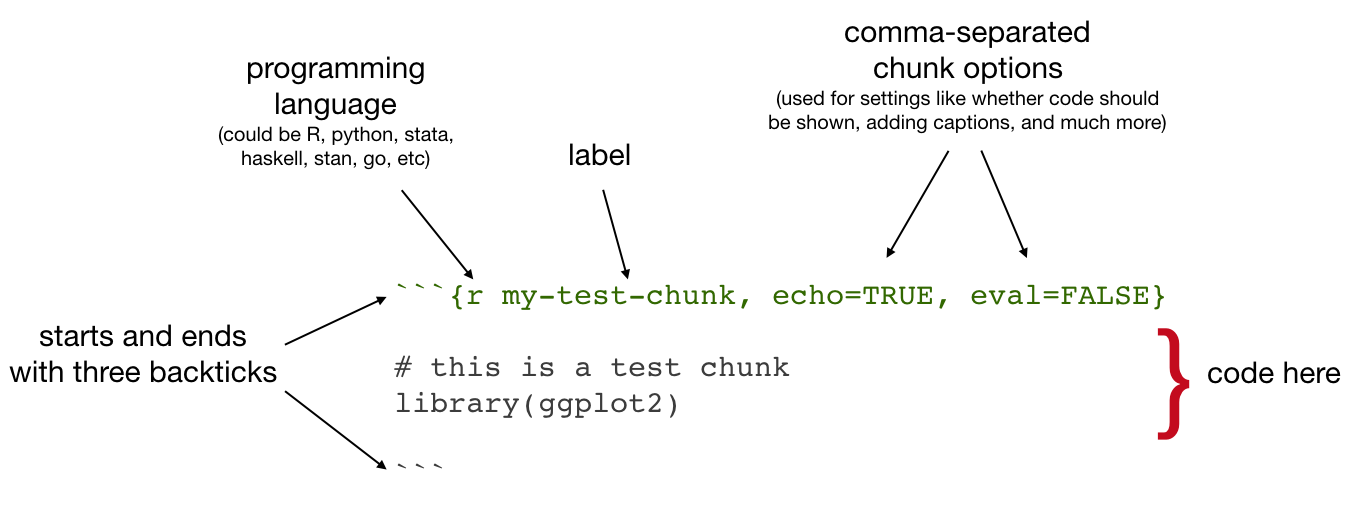
\includegraphics[width=1\linewidth]{figures/sample-content/chunk-parts} \caption{Code chunk syntax}\label{fig:chunk-parts}
\end{figure}

Le opzioni di blocco comuni includono (vedi ad esempio \href{https://bookdown.org/yihui/rmarkdown/r-code.html}{bookdown.org}):

\begin{itemize}
\tightlist
\item
  \texttt{echo}: se visualizzare o meno il codice nell'output knitted
\item
  \texttt{eval}: se o per eseguire il codice nel blocco durante il lavoro a maglia
\item
  \texttt{include}: se includere qualcosa da un pezzo di codice nel documento di output
\item
  \texttt{fig.cap}: didascalia della figura
\item
  \texttt{fig.scap}: didascalia con cifre brevi, che verrà utilizzata nell'``Elenco delle cifre'' nella prima parte del PDF
\end{itemize}

\textbf{IMPORTANTE}: \emph{non} utilizzare i trattini bassi nelle etichette dei blocchi - se lo fai, è probabile che venga visualizzato un errore nell'output PDF che dice qualcosa come ``! Errore didascalia pacchetto: \textbackslash caption outside float''.

\hypertarget{pezzi-di-configurazione-configurazione-immagini-grafici}{%
\subsection{Pezzi di configurazione: configurazione, immagini, grafici}\label{pezzi-di-configurazione-configurazione-immagini-grafici}}

Un documento R Markdown di solito inizia con un pezzo che viene utilizzato per \textbf{caricare le librerie} e per \textbf{impostare le opzioni di blocco predefinite} con \texttt{knitr::opts\_chunk\$set}.

Nella tua tesi, questo accadrà probabilmente in \textbf{index.Rmd} e/o come parti di apertura in ciascuno dei tuoi capitoli.

\begin{verbatim}
```{r setup, include=FALSE}
# don't show code unless we explicitly set echo = TRUE
knitr::opts_chunk$set(echo = FALSE)

library(tidyverse)
```
\end{verbatim}

\hypertarget{comprese-le-immagini}{%
\subsection{Comprese le immagini}\label{comprese-le-immagini}}

I blocchi di codice vengono utilizzati anche per includere immagini, con \texttt{include\_graphics} dal pacchetto \texttt{knitr}, come in Figura \ref{fig:catto-logo}

\begin{Shaded}
\begin{Highlighting}[]
\NormalTok{knitr}\SpecialCharTok{::}\FunctionTok{include\_graphics}\NormalTok{(}\StringTok{"figures/sample{-}content/cattolica{-}logo.png"}\NormalTok{)}
\end{Highlighting}
\end{Shaded}

\begin{figure}

{\centering 
\includegraphics[width=0.5\linewidth]{figures/sample-content/cattolica-logo} 

}

\caption{UCSC logo}\label{fig:catto-logo}
\end{figure}

Utili opzioni di blocco per le figure includono:

\begin{itemize}
\tightlist
\item
  \texttt{out.width} (usare con una percentuale) per impostare la dimensione dell'immagine
\item
  se hai un'immagine che diventa mooolto grande nel tuo output, sarà vincolata alla larghezza della pagina impostando \texttt{out.width\ =\ "100\%"}
\end{itemize}

\hypertarget{rotazione-figura}{%
\subsubsection*{Rotazione figura}\label{rotazione-figura}}
\addcontentsline{toc}{subsubsection}{Rotazione figura}

Puoi usare l'opzione chunk \texttt{out.extra} per ruotare le immagini.

La sintassi è diversa per LaTeX e HTML, quindi per comodità potremmo iniziare assegnando la stringa giusta a una variabile che dipende dal formato in cui stai eseguendo l'output:

\begin{Shaded}
\begin{Highlighting}[]
\ControlFlowTok{if}\NormalTok{ (knitr}\SpecialCharTok{::}\FunctionTok{is\_latex\_output}\NormalTok{())\{}
\NormalTok{  rotate180 }\OtherTok{\textless{}{-}} \StringTok{"angle=180"}
\NormalTok{\} }\ControlFlowTok{else}\NormalTok{ \{}
\NormalTok{  rotate180 }\OtherTok{\textless{}{-}} \StringTok{"style=\textquotesingle{}transform:rotate(180deg);\textquotesingle{}"}
\NormalTok{\}}
\end{Highlighting}
\end{Shaded}

Quindi puoi fare riferimento a quella variabile come il valore di \texttt{out.extra} per ruotare le immagini, come in Figura \ref{fig:catto-logo-rotated}.

\begin{figure}

{\centering 
\includegraphics[width=0.5\linewidth,angle=180]{figures/sample-content/cattolica-logo} 

}

\caption{UCSC logo, rotated}\label{fig:catto-logo-rotated}
\end{figure}

\hypertarget{mettere-i-grafici}{%
\subsection{Mettere i grafici}\label{mettere-i-grafici}}

Allo stesso modo, i blocchi di codice vengono utilizzati per includere grafici generati dinamicamente.
Usi il codice ordinario in R o in altri linguaggi - La figura \ref{fig:cars-plot} mostra un grafico del set di dati \texttt{cars} delle distanze di arresto per le auto a varie velocità (questo set di dati è integrato in \textbf{R} ).

\begin{Shaded}
\begin{Highlighting}[]
\NormalTok{cars }\SpecialCharTok{\%\textgreater{}\%} 
  \FunctionTok{ggplot}\NormalTok{() }\SpecialCharTok{+}
    \FunctionTok{aes}\NormalTok{(}\AttributeTok{x =}\NormalTok{ speed, }\AttributeTok{y =}\NormalTok{ dist) }\SpecialCharTok{+}
    \FunctionTok{geom\_point}\NormalTok{()}
\end{Highlighting}
\end{Shaded}

\begin{figure}
\centering
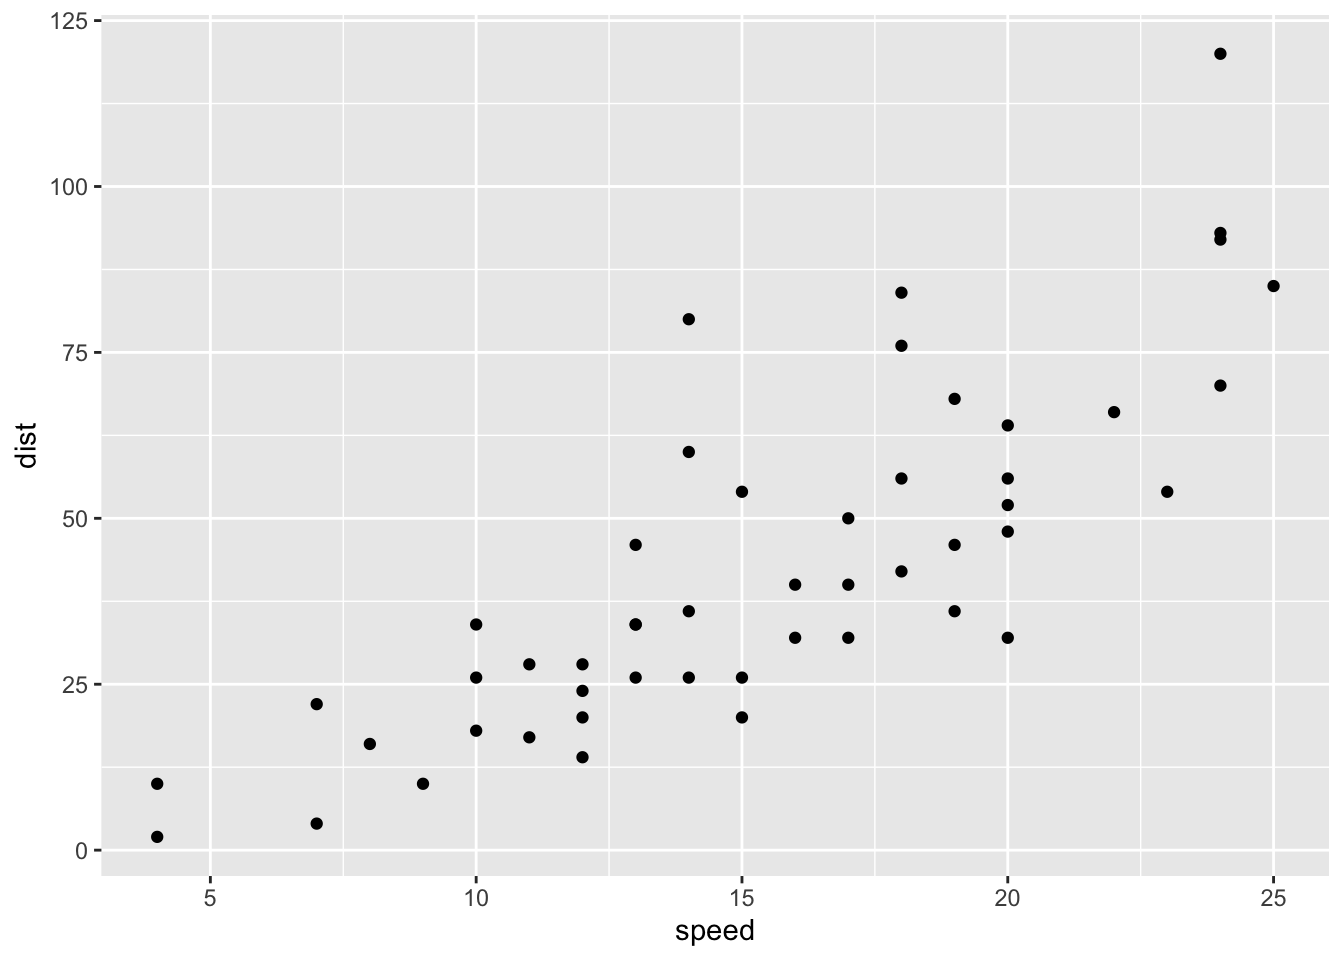
\includegraphics{_main_files/figure-latex/cars-plot-1.pdf}
\caption{\label{fig:cars-plot}A ggplot of car stuff}
\end{figure}

In automatico il grafico viene incluse nel tuo documento, così come le immagini. Questo succede tutte le volte che costruisci i.e.~buildi il libro (bookdown \texttt{bookdown::serve\_book()}) o fai knit i.e.\texttt{knitr::knit} un capitolo, i plots vengono generati automaticamente a partire dal tuo codice, poi salvati come immagini, quindi inclusi nel documento di output.

\hypertarget{tabelle}{%
\subsection{Tabelle}\label{tabelle}}

Le tabelle sono solitamente incluse con la funzione \texttt{kable} del pacchetto \texttt{knitr}.

La tabella \ref{tab:cars-table} mostra le prime righe dei dati del dataset \texttt{mtcars}.

\begin{Shaded}
\begin{Highlighting}[]
\NormalTok{cars }\SpecialCharTok{\%\textgreater{}\%} 
  \FunctionTok{head}\NormalTok{() }\SpecialCharTok{\%\textgreater{}\%} 
\NormalTok{  knitr}\SpecialCharTok{::}\FunctionTok{kable}\NormalTok{(}\AttributeTok{caption =} \StringTok{"A knitr kable table"}\NormalTok{)}
\end{Highlighting}
\end{Shaded}

\begin{table}

\caption{\label{tab:cars-table}A knitr kable table}
\centering
\begin{tabular}[t]{r|r}
\hline
speed & dist\\
\hline
4 & 2\\
\hline
4 & 10\\
\hline
7 & 4\\
\hline
7 & 22\\
\hline
8 & 16\\
\hline
9 & 10\\
\hline
\end{tabular}
\end{table}

\begin{itemize}
\tightlist
\item
  Gotchas: quando si utilizza \href{https://www.rdocumentation.org/packages/knitr/versions/1.21/topics/kable}{\texttt{kable}}, i sottotitoli sono impostati all'interno della funzione \texttt{kable}
\item
  Il pacchetto \texttt{kable} viene spesso utilizzato con il pacchetto \href{https://cran.r-project.org/web/packages/kableExtra/vignettes/awesome_table_in_html.html}{\texttt{kableExtra}}
\end{itemize}

\hypertarget{controllo-del-posizionamento}{%
\subsection{Controllo del posizionamento}\label{controllo-del-posizionamento}}

Una cosa che potrebbe essere fastidiosa è il modo in cui \emph{R Markdown} gestisce i ``fluttuanti'' come tabelle e figure. Li chiamo fluttuanti perchè prendo a prestito la notazione LaTeX che li chiama proprio così.
Nel tuo output PDF, LaTeX cercherà di trovare il posto migliore per mettere il tuo oggetto in base al testo che lo circonda e finché non hai davvero finito di scrivere dovresti semplicemente lasciarlo dove si trova.

In generale, dovresti consentire a LaTeX di farlo, ma se hai davvero \emph{veramente} bisogno di una figura da posizionare dove inserisci nel documento, puoi fare in modo che LaTeX tenti di farlo con l'opzione chunk \texttt{fig.pos="\ H"}, come in Figura \ref{fig:cattolica-logo-controlled}:

\begin{Shaded}
\begin{Highlighting}[]
\NormalTok{knitr}\SpecialCharTok{::}\FunctionTok{include\_graphics}\NormalTok{(}\StringTok{"figures/sample{-}content/cattolica{-}logo.png"}\NormalTok{)}
\end{Highlighting}
\end{Shaded}

\begin{figure}[H]

{\centering 
\includegraphics[width=0.5\linewidth]{figures/sample-content/cattolica-logo} 

}

\caption{An UCSC logo that LaTeX will try to place at this position in the text}\label{fig:cattolica-logo-controlled}
\end{figure}

Come sa chiunque abbia provato a giocare manualmente con il posizionamento di figure in un documento di Word, questo può avere effetti collaterali tipo spaziatura extra su altre pagine, ecc.
Pertanto, generalmente non è una buona idea farlo - fallo solo quando hai davvero bisogno di assicurarti che un'immagine segua direttamente sotto il testo dove ti riferisci ad essa (in questo documento, dovevo farlo per Figure @ref( fig:latex-font-sizing) nella sezione \ref{max-power}).
Per maggiori dettagli, leggi la sezione pertinente del \href{https://bookdown.org/yihui/rmarkdown-cookbook/figure-placement.html}{R Markdown Cookbook}.

\hypertarget{codice-in-linea-eseguibile}{%
\section{Codice in linea eseguibile}\label{codice-in-linea-eseguibile}}

``Codice in linea'' significa semplicemente inclusione di codice all'interno del testo.
La sintassi per farlo è \texttt{\textasciigrave{}r\ R\_CODE\textasciigrave{}}
Ad esempio, \texttt{\textasciigrave{}r\ 4\ +\ 4\textasciigrave{}} produrrà 8 nel tuo testo.

Di solito lo utilizzerai nelle parti della tua tesi in cui riporti i risultati: leggi i dati o i risultati in un blocco di codice, archivia le cose che vuoi segnalare in una variabile, quindi inserisci il valore di quella variabile nel tuo testo.
Ad esempio, potremmo assegnare il numero di righe nel dataset \texttt{cars} a una variabile:

\begin{Shaded}
\begin{Highlighting}[]
\NormalTok{num\_car\_observations }\OtherTok{\textless{}{-}} \FunctionTok{nrow}\NormalTok{(cars)}
\end{Highlighting}
\end{Shaded}

Potremmo quindi scrivere:\\
``Nel set di dati \texttt{cars}, abbiamo osservazioni \texttt{\textasciigrave{}r\ num\_car\_observations\textasciigrave{}}.''

Che genererebbe:\\
``Nel set di dati \texttt{cars}, abbiamo osservazioni 50.''

\hypertarget{codice-eseguibile-in-linguaggi-diversi-da-r}{%
\section{Codice eseguibile in linguaggi diversi da R}\label{codice-eseguibile-in-linguaggi-diversi-da-r}}

Se desideri utilizzare linguaggi diversi da R, come Python, Julia C++ o SQL, consulta \href{https://bookdown.org/yihui/rmarkdown-cookbook/other-\%20lingue.html}{la sezione pertinente del \emph{R Markdown Cookbook}}.

\hypertarget{cites-and-refs}{%
\chapter{Citazioni, referenze incrociate, e collaborazione}\label{cites-and-refs}}

\chaptermark{Citations and cross-refs}

\minitoc 

\hypertarget{citazioni}{%
\section{Citazioni}\label{citazioni}}

Il modo per includere le citazioni in un documento \emph{R Markdown} è inserire i riferimenti in un file di testo normale con estensione \textbf{.bib}, in formato \textbf{BibTex}.\footnote{la bibliografia può essere anche in altri formati, inclusi EndNote (\textbf{.enl}) e RIS (\textbf{.ris}), vedere \href{https\%20://rmarkdown.rstudio.com/authoring_bibliographies_and_citations.html}{rmarkdown.rstudio.com/authoring\_bibliographies\_and\_citations}.}
Quindi fai riferimento al percorso di questo file nell'intestazione YAML di \textbf{index.Rmd} con \texttt{bibliography:\ example.bib}.

La maggior parte dei gestori di referenze può creare automaticamente un file .bib con le tue referenze.
Tuttavia, il \textbf{di gran lunga} miglior gestore di riferimento da utilizzare con \emph{R Markdown} è \href{https://www.zotero.org}{Zotero} con il \href{https://retorque.\%20re/zotero-better-bibtex/}{plug-in Better BibTex}, perché il plugin \texttt{citr} per RStudio (vedi sotto) può leggere i riferimenti direttamente dalla tua libreria Zotero!
Ah, dimenticavo, Rmarkdown sistema da sola in ordine alfabetico le referenze ogni volta che fai knit e ne fai riferimento nel testo. Puoi dare un'occhiata anche a \href{https://www.mybib.com/\#/}{mybib}, molto comodo e ti permette di esportare nel formato che più preferisci.

Ecco un esempio di una voce in un file \textbf{.bib}:

\begin{Shaded}
\begin{Highlighting}[]
\VariableTok{@article}\NormalTok{\{}\OtherTok{Shea2014}\NormalTok{,}
  \DataTypeTok{author}\NormalTok{ =        \{Shea, Nicholas and Boldt, Annika\},}
  \DataTypeTok{journal}\NormalTok{ =       \{Trends in Cognitive Sciences\},}
  \DataTypeTok{pages}\NormalTok{ =         \{186{-}{-}193\},}
  \DataTypeTok{title}\NormalTok{ =         \{\{Supra{-}personal cognitive control\}\},}
  \DataTypeTok{volume}\NormalTok{ =        \{18\},}
  \DataTypeTok{year}\NormalTok{ =          \{2014\},}
  \DataTypeTok{doi}\NormalTok{ =           \{10.1016/j.tics.2014.01.006\},}
\NormalTok{\}}
\end{Highlighting}
\end{Shaded}

In questa sezione evidenziata, `Shea2014' è l'\textbf{identificativo di citazione}.
Il modo predefinito per citare una voce nel testo è con questa sintassi: \texttt{{[}@citation-identifier{]}}.

Quindi potrai citare alcune referenze così (\protect\hyperlink{ref-Lottridge2012}{Lottridge et al., 2012}; \protect\hyperlink{ref-Mill1965}{Mill, 1965 {[}1843{]}}; \protect\hyperlink{ref-Shea2014}{Shea et al., 2014}).

\hypertarget{citation-appearance}{%
\subsection{Aspetto delle citazioni e della sezione dei riferimenti (pandoc)}\label{citation-appearance}}

Per una impostazione predefinita, \texttt{cattolicadown} consente a \href{https://pandoc.org}{Pandoc} di gestire il modo in cui le citazioni vengono inserite nel testo e nella sezione dei riferimenti.
Puoi modificare l'aspetto di citazioni e riferimenti specificando un file CSL (Citation Style Language) nel campo dei metadati \texttt{csl} di \textbf{index.Rmd}.
Per impostazione predefinita, ``cattolica'' dell'American Psychological Association APA (7a edizione).

Con questo stile, è utile conoscere una serie di variazioni sulla sintassi della citazione:

\begin{itemize}
\tightlist
\item
  Metti i nomi degli autori fuori parentesi

  \begin{itemize}
  \tightlist
  \item
    Questo: \texttt{@Shea2014\ dice\ bla.}
  \item
    Diventa: Shea et al. (\protect\hyperlink{ref-Shea2014}{2014}) dice bla.
  \end{itemize}
\item
  Includere solo l'anno di citazione (tra parentesi)

  \begin{itemize}
  \tightlist
  \item
    Questo: \texttt{Shea\ et\ al.\ dice\ bla\ {[}-@Shea2014{]}}
  \item
    Diventa: Shea et al.~dice bla (\protect\hyperlink{ref-Shea2014}{2014})
  \end{itemize}
\item
  Aggiungi testo e riferimenti a pagine o capitoli alla citazione

  \begin{itemize}
  \tightlist
  \item
    Questo: \texttt{{[}vedi\ @Shea2014,\ pp.\ 33-35;\ anche\ @Wu2016,\ cap.\ 1{]}}
  \item
    Diventa: bla bla (vedi \protect\hyperlink{ref-Shea2014}{Shea et al., 2014, pp. 33--35}; anche \protect\hyperlink{ref-Wu2016}{Wu, 2016}, cap. 1).
  \end{itemize}
\end{itemize}

Se invece vuoi uno stile di citazione con numero, prova \texttt{csl:\ bibliography/transactions-on-computer-human-interaction.csl} o sfoglia semplicemente il \href{https://www.zotero.org/\%20stili}{Zotero Style Repository} cercando uno che ti piace.
Per comodità, puoi impostare l'interlinea e lo spazio tra le voci bibliografiche nella sezione di riferimento direttamente dall'intestazione YAML in \textbf{index.Rmd}.

Se preferisci usare \texttt{bilatex} o \texttt{natbib} per gestire i riferimenti, vedi \protect\hyperlink{customising-citations}{questo capitolo}.
\clearpage

\hypertarget{inserisci-facilmente-i-riferimenti-con-leditor-visivo-di-rstudio}{%
\subsection{Inserisci facilmente i riferimenti con l'editor visivo di RStudio}\label{inserisci-facilmente-i-riferimenti-con-leditor-visivo-di-rstudio}}

Per inserire facilmente le citazioni, usa il {[}Visual Editor{]} di RStudio (\url{https://rstudio.github.io/visual-markdown-editing/citations.html}).
Assicurati di avere l'ultima versione di RStudio: l'editor visivo originariamente era davvero buggato, specialmente in relazione ai riferimenti, ma v2022.02.0 è fantastico!

\hypertarget{riferimenti-incrociati}{%
\section{Riferimenti incrociati}\label{riferimenti-incrociati}}

Possiamo fare riferimenti incrociati a \textbf{sezioni} all'interno del nostro documento, nonché a \textbf{figure} (immagini e grafici) e \textbf{tabelle}.

La sintassi generale per i riferimenti incrociati è \textbf{\texttt{\textbackslash{}@ref(label)}}

\hypertarget{riferimenti-alla-sezione}{%
\subsection{Riferimenti alla sezione}\label{riferimenti-alla-sezione}}

Alle intestazioni viene assegnata automaticamente un'etichetta di riferimento, che è il testo in maiuscolo separato da trattini. Ad esempio, a \texttt{\#\ My\ header} viene assegnata automaticamente l'etichetta \texttt{my-header}. Quindi \texttt{\#\ My\ header} può essere referenziato con \texttt{\textbackslash{}@ref(my-section)}

Ricordi cosa abbiamo scritto nella sezione \ref{citations}?

Possiamo anche usare la \textbf{sintassi del collegamento ipertestuale} e aggiungere \# prima dell'etichetta, anche se questo è garantito che funzioni correttamente solo nell'output HTML:

\begin{itemize}
\tightlist
\item
  Quindi se scriviamo \texttt{Ricordi\ cosa\ abbiamo\ scritto\ nella\ {[}sezione\ precedente{]}(\#citations)?}
\item
  Diventa Ricorda cosa abbiamo scritto nella \protect\hyperlink{citations}{sezione precedente}?
\end{itemize}

\hypertarget{creazione-di-etichette-personalizzate}{%
\subsubsection{Creazione di etichette personalizzate}\label{creazione-di-etichette-personalizzate}}

È un'ottima idea creare \textbf{etichette personalizzate} per le nostre sezioni. Questo perché le etichette assegnate automaticamente cambieranno quando cambiamo i titoli delle sezioni - per evitare ciò, possiamo creare noi stessi le etichette e lasciarle intatte se cambiamo i titoli delle sezioni.

Creiamo etichette personalizzate aggiungendo \texttt{\{\#label\}} dopo un'intestazione, ad es. \texttt{\#\ La\ mia\ sezione\ \{\#my-label\}}.
Vedi \protect\hyperlink{cites-and-refs}{il titolo del nostro capitolo} per un esempio. Quella era la sezione \ref{cites-and-refs}.

\hypertarget{riferimenti-a-figure-immagine-e-grafico.}{%
\subsection{Riferimenti a figure (immagine e grafico).}\label{riferimenti-a-figure-immagine-e-grafico.}}

\begin{itemize}
\tightlist
\item
  Per fare riferimento a figure (ovvero immagini e grafici) utilizzare la sintassi \texttt{\textbackslash{}@ref(fig:label)}
\item
  \textbf{NB}: le figure e le tabelle devono avere didascalie se desideri fare un riferimento incrociato.
\end{itemize}

Aggiungiamo un'immagine:

\begin{Shaded}
\begin{Highlighting}[]
\NormalTok{knitr}\SpecialCharTok{::}\FunctionTok{include\_graphics}\NormalTok{(}\StringTok{"figures/sample{-}content/captain.jpeg"}\NormalTok{)}
\end{Highlighting}
\end{Shaded}

\begin{figure}

{\centering 
\includegraphics[width=0.65\linewidth]{figures/sample-content/captain} 

}

\caption{A marvel-lous meme}\label{fig:capitano}
\end{figure}

Ci riferiamo a questa immagine con \texttt{\textbackslash{}@ref(fig:capitano)}.
Quindi la figura \ref{fig:capitano} è \protect\hyperlink{fig:capitano}{questa immagine}.

E nella figura \ref{fig:cars-plot} vediamo \protect\hyperlink{fig:cars-plot}{cars plot}.

\hypertarget{riferimenti-a-tabelle}{%
\subsection{Riferimenti a tabelle}\label{riferimenti-a-tabelle}}

\begin{itemize}
\tightlist
\item
  Per fare riferimento alle tabelle, utilizzare la sintassi \texttt{\textbackslash{}@ref(tab:label)}
\end{itemize}

Adesso includiamo la tabella:

\begin{Shaded}
\begin{Highlighting}[]
\NormalTok{knitr}\SpecialCharTok{::}\FunctionTok{kable}\NormalTok{(cars[}\DecValTok{1}\SpecialCharTok{:}\DecValTok{5}\NormalTok{,],}
            \AttributeTok{caption=}\StringTok{"Stopping cars"}\NormalTok{)}
\end{Highlighting}
\end{Shaded}

\begin{table}

\caption{\label{tab:cars-table2}Stopping cars}
\centering
\begin{tabular}[t]{r|r}
\hline
speed & dist\\
\hline
4 & 2\\
\hline
4 & 10\\
\hline
7 & 4\\
\hline
7 & 22\\
\hline
8 & 16\\
\hline
\end{tabular}
\end{table}

Ci riferiamo a questa tabella con \texttt{\textbackslash{}@ref(tab:cars-table2)}.
Quindi la tabella \ref{tab:cars-table2} è \protect\hyperlink{tab:cars-table2}{questa tabella}.

E nella tabella \ref{tab:cars-table} abbiamo visto più o meno \protect\hyperlink{tab:cars-table}{la stessa tabella delle auto}.

\hypertarget{numeri-di-pagina}{%
\subsection{Numeri di pagina}\label{numeri-di-pagina}}

Infine, nell'output PDF potremmo anche voler includere il numero di pagina di un riferimento, in modo che sia facile trovarlo nell'output fisico stampato.
LaTeX ha un comando per questo, che assomiglia a questo: \texttt{\textbackslash{}pageref\{fig/tab:label\}} (nota: parentesi graffe, non parentesi)

Quando eseguiamo l'output in PDF, possiamo utilizzare LaTeX non elaborato direttamente nei nostri file .Rmd. Quindi se volessimo inserirenil grafico della auto alla pagina potremmo scrivere:

\begin{itemize}
\tightlist
\item
  Questo: \texttt{Figura\ \textbackslash{}@ref(fig:cars-plot)\ nella\ pagina\ \textbackslash{}pageref(fig:cars-plot)}
\item
  Diventa: Figura \ref{fig:cars-plot} nella pagina \pageref{fig:cars-plot}
\end{itemize}

\hypertarget{numeri-di-pagina-solo-nelloutput-pdf}{%
\subsubsection{Numeri di pagina solo nell'output PDF}\label{numeri-di-pagina-solo-nelloutput-pdf}}

Un problema qui è che i comandi LaTeX non vengono visualizzati nell'output HTML, ma anche nell'output di gitbook, da cui osserveremo ``Figure \ref{fig:cars-plot} on page''.

Un modo per aggirare questo problema è utilizzare il codice inline per inserire il testo e utilizzare un'istruzione \texttt{ifelse} per controllare il formato di output e quindi inserire il testo appropriato solo se conforme al formato desiderato.

\begin{itemize}
\tightlist
\item
  Quindi: \texttt{\textasciigrave{}r\ ifelse(knitr::is\_latex\_output(),\ "Figure\ \textbackslash{}\textbackslash{}@ref(fig:cars-plot)\ on\ page\ \textbackslash{}\textbackslash{}pageref\{fig:cars-plot\}",\ "")\textasciigrave{}}
\item
  Inserisci questo (verifica che sia solo PDF output): Figure \ref{fig:cars-plot} on page \pageref{fig:cars-plot}
\end{itemize}

Si noti che è necessario eseguire l'escape della barra inversa con un'altra barra inversa qui per ottenere l'output corretto.

\hypertarget{scrittura-collaborativa}{%
\section{Scrittura collaborativa}\label{scrittura-collaborativa}}

Le migliori pratiche per la collaborazione e il rilevamento delle modifiche quando si utilizza R Markdown sono ancora una questione aperta.
Nel post del blog \href{https://livefreeordichotomize.com/2018/09/14/one-year-to-dissertate/}{\textbf{One year to dissertate}} di Lucy D'Agostino, che consiglio vivamente, l'autorice unisce i file .Rmd a un documento di Word, quindi utilizza il pacchetto ``googledrive'' R per inviarlo a Google Drive per commenti / revisioni dai coautori, quindi incorpora i suggerimenti di Google Drive \emph{a mano} nel sorgente .Rmd File.
Questo approccio è un po' goffo e ci sono discussioni in corso tra gli sviluppatori di \emph{R Markdown} su quale sia il modo migliore per gestire la scrittura collaborativa (vedi \href{https://github.com/rstudio/rmarkdown/issues/1463}{numero \#1463} su GitHub, dove \href{http://criticmarkup.com}{CriticMarkup} è tra i suggerimenti).

Per ora, questa è una domanda aperta nella comunità degli utenti di R Markdown.
Spesso lavoro a un formato che può essere facilmente importato in Google Docs per i commenti, quindi esamino le revisioni suggerite e le reinserisco manualmente nei file di origine .Rmd.
Per gli articoli, a volte carico una bozza quasi definitiva su \href{https://www.overleaf.com/}{Overleaf}, quindi apporto in modo collaborativo le modifiche finali al file LaTeX lì.
Sospetto che qualche grande soluzione sarà sviluppata in un futuro non troppo lontano, probabilmente dal team di RStudio.

\hypertarget{risorse-addizionali}{%
\section{Risorse addizionali}\label{risorse-addizionali}}

\begin{itemize}
\item
  \emph{R Markdown: The Definitive Guide} - \url{https://bookdown.org/yihui/rmarkdown/}
\item
  \emph{R for Data Science} - \url{https://r4ds.had.co.nz}
\end{itemize}

\hypertarget{tables}{%
\chapter{Tabelle}\label{tables}}

\minitoc 

\hypertarget{fare-in-modo-che-le-tabelle-latex-si-comportino-bene}{%
\section{Fare in modo che le tabelle LaTeX si comportino bene}\label{fare-in-modo-che-le-tabelle-latex-si-comportino-bene}}

Gestire le tabelle in LaTeX può essere disgustoso.
Questa sezione spiega i principali trucchi di cui hai bisogno per evitare di accumulare stress.

(Nota: se stai guardando la versione ebook, non vedrai molte differenze in questa sezione, poiché è rilevante solo per l'output PDF!)

\hypertarget{rendere-bella-la-tua-tabella}{%
\subsection{Rendere bella la tua tabella}\label{rendere-bella-la-tua-tabella}}

Quando usi \texttt{kable} per creare tabelle, quasi sicuramente vorrai impostare l'opzione \texttt{booktabs\ =\ TRUE}.
Questo già e sufficiente a renderla presentabile:

\begin{Shaded}
\begin{Highlighting}[]
\FunctionTok{library}\NormalTok{(knitr)}
\FunctionTok{library}\NormalTok{(tidyverse)}

\FunctionTok{head}\NormalTok{(mtcars) }\SpecialCharTok{\%\textgreater{}\%} 
  \FunctionTok{kable}\NormalTok{(}\AttributeTok{booktabs =} \ConstantTok{TRUE}\NormalTok{)}
\end{Highlighting}
\end{Shaded}

\begin{tabular}{lrrrrrrrrrrr}
\toprule
  & mpg & cyl & disp & hp & drat & wt & qsec & vs & am & gear & carb\\
\midrule
Mazda RX4 & 21.0 & 6 & 160 & 110 & 3.90 & 2.620 & 16.46 & 0 & 1 & 4 & 4\\
Mazda RX4 Wag & 21.0 & 6 & 160 & 110 & 3.90 & 2.875 & 17.02 & 0 & 1 & 4 & 4\\
Datsun 710 & 22.8 & 4 & 108 & 93 & 3.85 & 2.320 & 18.61 & 1 & 1 & 4 & 1\\
Hornet 4 Drive & 21.4 & 6 & 258 & 110 & 3.08 & 3.215 & 19.44 & 1 & 0 & 3 & 1\\
Hornet Sportabout & 18.7 & 8 & 360 & 175 & 3.15 & 3.440 & 17.02 & 0 & 0 & 3 & 2\\
\addlinespace
Valiant & 18.1 & 6 & 225 & 105 & 2.76 & 3.460 & 20.22 & 1 & 0 & 3 & 1\\
\bottomrule
\end{tabular}

\vspace{4mm}

Dai un'occhiata q questa con lo stile predefinito, è orribile:

\begin{Shaded}
\begin{Highlighting}[]
\FunctionTok{head}\NormalTok{(mtcars) }\SpecialCharTok{\%\textgreater{}\%} 
  \FunctionTok{kable}\NormalTok{()}
\end{Highlighting}
\end{Shaded}

\begin{tabular}{l|r|r|r|r|r|r|r|r|r|r|r}
\hline
  & mpg & cyl & disp & hp & drat & wt & qsec & vs & am & gear & carb\\
\hline
Mazda RX4 & 21.0 & 6 & 160 & 110 & 3.90 & 2.620 & 16.46 & 0 & 1 & 4 & 4\\
\hline
Mazda RX4 Wag & 21.0 & 6 & 160 & 110 & 3.90 & 2.875 & 17.02 & 0 & 1 & 4 & 4\\
\hline
Datsun 710 & 22.8 & 4 & 108 & 93 & 3.85 & 2.320 & 18.61 & 1 & 1 & 4 & 1\\
\hline
Hornet 4 Drive & 21.4 & 6 & 258 & 110 & 3.08 & 3.215 & 19.44 & 1 & 0 & 3 & 1\\
\hline
Hornet Sportabout & 18.7 & 8 & 360 & 175 & 3.15 & 3.440 & 17.02 & 0 & 0 & 3 & 2\\
\hline
Valiant & 18.1 & 6 & 225 & 105 & 2.76 & 3.460 & 20.22 & 1 & 0 & 3 & 1\\
\hline
\end{tabular}

\hypertarget{se-il-tuo-tavolo-uxe8-troppo-largo}{%
\subsection{Se il tuo tavolo è troppo largo}\label{se-il-tuo-tavolo-uxe8-troppo-largo}}

Potresti scoprire che la tua tabella si espande oltre i margini della pagina, come le tabelle sopra.
Risolvi questo problema con la funzione \texttt{kable\_styling} dal pacchetto \href{https://haozhu233.github.io/kableExtra/}{\texttt{kableExtra}}:

\begin{Shaded}
\begin{Highlighting}[]
\FunctionTok{library}\NormalTok{(kableExtra)}

\FunctionTok{head}\NormalTok{(mtcars) }\SpecialCharTok{\%\textgreater{}\%} 
  \FunctionTok{kable}\NormalTok{(}\AttributeTok{booktabs =} \ConstantTok{TRUE}\NormalTok{) }\SpecialCharTok{\%\textgreater{}\%} 
  \FunctionTok{kable\_styling}\NormalTok{(}\AttributeTok{latex\_options =} \StringTok{"scale\_down"}\NormalTok{)}
\end{Highlighting}
\end{Shaded}

\begin{table}
\centering
\resizebox{\linewidth}{!}{
\begin{tabular}{lrrrrrrrrrrr}
\toprule
  & mpg & cyl & disp & hp & drat & wt & qsec & vs & am & gear & carb\\
\midrule
Mazda RX4 & 21.0 & 6 & 160 & 110 & 3.90 & 2.620 & 16.46 & 0 & 1 & 4 & 4\\
Mazda RX4 Wag & 21.0 & 6 & 160 & 110 & 3.90 & 2.875 & 17.02 & 0 & 1 & 4 & 4\\
Datsun 710 & 22.8 & 4 & 108 & 93 & 3.85 & 2.320 & 18.61 & 1 & 1 & 4 & 1\\
Hornet 4 Drive & 21.4 & 6 & 258 & 110 & 3.08 & 3.215 & 19.44 & 1 & 0 & 3 & 1\\
Hornet Sportabout & 18.7 & 8 & 360 & 175 & 3.15 & 3.440 & 17.02 & 0 & 0 & 3 & 2\\
\addlinespace
Valiant & 18.1 & 6 & 225 & 105 & 2.76 & 3.460 & 20.22 & 1 & 0 & 3 & 1\\
\bottomrule
\end{tabular}}
\end{table}

Questo ridimensiona la tabella per adattarsi alla larghezza della pagina.

\hypertarget{se-la-tabella-uxe8-troppo-lunga}{%
\subsection{Se la tabella è troppo lunga}\label{se-la-tabella-uxe8-troppo-lunga}}

Se la tua tabella è troppo lunga per stare su una singola pagina, imposta \texttt{longtable\ =\ TRUE} nella funzione \texttt{kable} per dividere la tabella su più pagine.

\begin{Shaded}
\begin{Highlighting}[]
\NormalTok{a\_long\_table }\OtherTok{\textless{}{-}} \FunctionTok{rbind}\NormalTok{(mtcars, mtcars)}

\NormalTok{a\_long\_table }\SpecialCharTok{\%\textgreater{}\%} 
  \FunctionTok{select}\NormalTok{(}\DecValTok{1}\SpecialCharTok{:}\DecValTok{8}\NormalTok{) }\SpecialCharTok{\%\textgreater{}\%} 
  \FunctionTok{kable}\NormalTok{(}\AttributeTok{booktabs =} \ConstantTok{TRUE}\NormalTok{, }\AttributeTok{longtable =} \ConstantTok{TRUE}\NormalTok{)}
\end{Highlighting}
\end{Shaded}

\begin{longtable}{lrrrrrrrr}
\toprule
  & mpg & cyl & disp & hp & drat & wt & qsec & vs\\
\midrule
Mazda RX4 & 21.0 & 6 & 160.0 & 110 & 3.90 & 2.620 & 16.46 & 0\\
Mazda RX4 Wag & 21.0 & 6 & 160.0 & 110 & 3.90 & 2.875 & 17.02 & 0\\
Datsun 710 & 22.8 & 4 & 108.0 & 93 & 3.85 & 2.320 & 18.61 & 1\\
Hornet 4 Drive & 21.4 & 6 & 258.0 & 110 & 3.08 & 3.215 & 19.44 & 1\\
Hornet Sportabout & 18.7 & 8 & 360.0 & 175 & 3.15 & 3.440 & 17.02 & 0\\
\addlinespace
Valiant & 18.1 & 6 & 225.0 & 105 & 2.76 & 3.460 & 20.22 & 1\\
Duster 360 & 14.3 & 8 & 360.0 & 245 & 3.21 & 3.570 & 15.84 & 0\\
Merc 240D & 24.4 & 4 & 146.7 & 62 & 3.69 & 3.190 & 20.00 & 1\\
Merc 230 & 22.8 & 4 & 140.8 & 95 & 3.92 & 3.150 & 22.90 & 1\\
Merc 280 & 19.2 & 6 & 167.6 & 123 & 3.92 & 3.440 & 18.30 & 1\\
\addlinespace
Merc 280C & 17.8 & 6 & 167.6 & 123 & 3.92 & 3.440 & 18.90 & 1\\
Merc 450SE & 16.4 & 8 & 275.8 & 180 & 3.07 & 4.070 & 17.40 & 0\\
Merc 450SL & 17.3 & 8 & 275.8 & 180 & 3.07 & 3.730 & 17.60 & 0\\
Merc 450SLC & 15.2 & 8 & 275.8 & 180 & 3.07 & 3.780 & 18.00 & 0\\
Cadillac Fleetwood & 10.4 & 8 & 472.0 & 205 & 2.93 & 5.250 & 17.98 & 0\\
\addlinespace
Lincoln Continental & 10.4 & 8 & 460.0 & 215 & 3.00 & 5.424 & 17.82 & 0\\
Chrysler Imperial & 14.7 & 8 & 440.0 & 230 & 3.23 & 5.345 & 17.42 & 0\\
Fiat 128 & 32.4 & 4 & 78.7 & 66 & 4.08 & 2.200 & 19.47 & 1\\
Honda Civic & 30.4 & 4 & 75.7 & 52 & 4.93 & 1.615 & 18.52 & 1\\
Toyota Corolla & 33.9 & 4 & 71.1 & 65 & 4.22 & 1.835 & 19.90 & 1\\
\addlinespace
Toyota Corona & 21.5 & 4 & 120.1 & 97 & 3.70 & 2.465 & 20.01 & 1\\
Dodge Challenger & 15.5 & 8 & 318.0 & 150 & 2.76 & 3.520 & 16.87 & 0\\
AMC Javelin & 15.2 & 8 & 304.0 & 150 & 3.15 & 3.435 & 17.30 & 0\\
Camaro Z28 & 13.3 & 8 & 350.0 & 245 & 3.73 & 3.840 & 15.41 & 0\\
Pontiac Firebird & 19.2 & 8 & 400.0 & 175 & 3.08 & 3.845 & 17.05 & 0\\
\addlinespace
Fiat X1-9 & 27.3 & 4 & 79.0 & 66 & 4.08 & 1.935 & 18.90 & 1\\
Porsche 914-2 & 26.0 & 4 & 120.3 & 91 & 4.43 & 2.140 & 16.70 & 0\\
Lotus Europa & 30.4 & 4 & 95.1 & 113 & 3.77 & 1.513 & 16.90 & 1\\
Ford Pantera L & 15.8 & 8 & 351.0 & 264 & 4.22 & 3.170 & 14.50 & 0\\
Ferrari Dino & 19.7 & 6 & 145.0 & 175 & 3.62 & 2.770 & 15.50 & 0\\
\addlinespace
Maserati Bora & 15.0 & 8 & 301.0 & 335 & 3.54 & 3.570 & 14.60 & 0\\
Volvo 142E & 21.4 & 4 & 121.0 & 109 & 4.11 & 2.780 & 18.60 & 1\\
Mazda RX41 & 21.0 & 6 & 160.0 & 110 & 3.90 & 2.620 & 16.46 & 0\\
Mazda RX4 Wag1 & 21.0 & 6 & 160.0 & 110 & 3.90 & 2.875 & 17.02 & 0\\
Datsun 7101 & 22.8 & 4 & 108.0 & 93 & 3.85 & 2.320 & 18.61 & 1\\
\addlinespace
Hornet 4 Drive1 & 21.4 & 6 & 258.0 & 110 & 3.08 & 3.215 & 19.44 & 1\\
Hornet Sportabout1 & 18.7 & 8 & 360.0 & 175 & 3.15 & 3.440 & 17.02 & 0\\
Valiant1 & 18.1 & 6 & 225.0 & 105 & 2.76 & 3.460 & 20.22 & 1\\
Duster 3601 & 14.3 & 8 & 360.0 & 245 & 3.21 & 3.570 & 15.84 & 0\\
Merc 240D1 & 24.4 & 4 & 146.7 & 62 & 3.69 & 3.190 & 20.00 & 1\\
\addlinespace
Merc 2301 & 22.8 & 4 & 140.8 & 95 & 3.92 & 3.150 & 22.90 & 1\\
Merc 2801 & 19.2 & 6 & 167.6 & 123 & 3.92 & 3.440 & 18.30 & 1\\
Merc 280C1 & 17.8 & 6 & 167.6 & 123 & 3.92 & 3.440 & 18.90 & 1\\
Merc 450SE1 & 16.4 & 8 & 275.8 & 180 & 3.07 & 4.070 & 17.40 & 0\\
Merc 450SL1 & 17.3 & 8 & 275.8 & 180 & 3.07 & 3.730 & 17.60 & 0\\
\addlinespace
Merc 450SLC1 & 15.2 & 8 & 275.8 & 180 & 3.07 & 3.780 & 18.00 & 0\\
Cadillac Fleetwood1 & 10.4 & 8 & 472.0 & 205 & 2.93 & 5.250 & 17.98 & 0\\
Lincoln Continental1 & 10.4 & 8 & 460.0 & 215 & 3.00 & 5.424 & 17.82 & 0\\
Chrysler Imperial1 & 14.7 & 8 & 440.0 & 230 & 3.23 & 5.345 & 17.42 & 0\\
Fiat 1281 & 32.4 & 4 & 78.7 & 66 & 4.08 & 2.200 & 19.47 & 1\\
\addlinespace
Honda Civic1 & 30.4 & 4 & 75.7 & 52 & 4.93 & 1.615 & 18.52 & 1\\
Toyota Corolla1 & 33.9 & 4 & 71.1 & 65 & 4.22 & 1.835 & 19.90 & 1\\
Toyota Corona1 & 21.5 & 4 & 120.1 & 97 & 3.70 & 2.465 & 20.01 & 1\\
Dodge Challenger1 & 15.5 & 8 & 318.0 & 150 & 2.76 & 3.520 & 16.87 & 0\\
AMC Javelin1 & 15.2 & 8 & 304.0 & 150 & 3.15 & 3.435 & 17.30 & 0\\
\addlinespace
Camaro Z281 & 13.3 & 8 & 350.0 & 245 & 3.73 & 3.840 & 15.41 & 0\\
Pontiac Firebird1 & 19.2 & 8 & 400.0 & 175 & 3.08 & 3.845 & 17.05 & 0\\
Fiat X1-91 & 27.3 & 4 & 79.0 & 66 & 4.08 & 1.935 & 18.90 & 1\\
Porsche 914-21 & 26.0 & 4 & 120.3 & 91 & 4.43 & 2.140 & 16.70 & 0\\
Lotus Europa1 & 30.4 & 4 & 95.1 & 113 & 3.77 & 1.513 & 16.90 & 1\\
\addlinespace
Ford Pantera L1 & 15.8 & 8 & 351.0 & 264 & 4.22 & 3.170 & 14.50 & 0\\
Ferrari Dino1 & 19.7 & 6 & 145.0 & 175 & 3.62 & 2.770 & 15.50 & 0\\
Maserati Bora1 & 15.0 & 8 & 301.0 & 335 & 3.54 & 3.570 & 14.60 & 0\\
Volvo 142E1 & 21.4 & 4 & 121.0 & 109 & 4.11 & 2.780 & 18.60 & 1\\
\bottomrule
\end{longtable}

Quando lo fai, probabilmente vorrai fare in modo che l'intestazione si ripeta su nuove pagine.
Fallo con la funzione \texttt{kable\_styling} di \texttt{kableExtra}:

\begin{Shaded}
\begin{Highlighting}[]
\NormalTok{a\_long\_table }\SpecialCharTok{\%\textgreater{}\%} 
  \FunctionTok{kable}\NormalTok{(}\AttributeTok{booktabs =} \ConstantTok{TRUE}\NormalTok{, }\AttributeTok{longtable =} \ConstantTok{TRUE}\NormalTok{) }\SpecialCharTok{\%\textgreater{}\%} 
  \FunctionTok{kable\_styling}\NormalTok{(}\AttributeTok{latex\_options =} \StringTok{"repeat\_header"}\NormalTok{)}
\end{Highlighting}
\end{Shaded}

\begin{longtable}{lrrrrrrrrrrr}
\toprule
  & mpg & cyl & disp & hp & drat & wt & qsec & vs & am & gear & carb\\
\midrule
\endfirsthead
\multicolumn{12}{@{}l}{\textit{(continued)}}\\
\toprule
  & mpg & cyl & disp & hp & drat & wt & qsec & vs & am & gear & carb\\
\midrule
\endhead

\endfoot
\bottomrule
\endlastfoot
Mazda RX4 & 21.0 & 6 & 160.0 & 110 & 3.90 & 2.620 & 16.46 & 0 & 1 & 4 & 4\\
Mazda RX4 Wag & 21.0 & 6 & 160.0 & 110 & 3.90 & 2.875 & 17.02 & 0 & 1 & 4 & 4\\
Datsun 710 & 22.8 & 4 & 108.0 & 93 & 3.85 & 2.320 & 18.61 & 1 & 1 & 4 & 1\\
Hornet 4 Drive & 21.4 & 6 & 258.0 & 110 & 3.08 & 3.215 & 19.44 & 1 & 0 & 3 & 1\\
Hornet Sportabout & 18.7 & 8 & 360.0 & 175 & 3.15 & 3.440 & 17.02 & 0 & 0 & 3 & 2\\
\addlinespace
Valiant & 18.1 & 6 & 225.0 & 105 & 2.76 & 3.460 & 20.22 & 1 & 0 & 3 & 1\\
Duster 360 & 14.3 & 8 & 360.0 & 245 & 3.21 & 3.570 & 15.84 & 0 & 0 & 3 & 4\\
Merc 240D & 24.4 & 4 & 146.7 & 62 & 3.69 & 3.190 & 20.00 & 1 & 0 & 4 & 2\\
Merc 230 & 22.8 & 4 & 140.8 & 95 & 3.92 & 3.150 & 22.90 & 1 & 0 & 4 & 2\\
Merc 280 & 19.2 & 6 & 167.6 & 123 & 3.92 & 3.440 & 18.30 & 1 & 0 & 4 & 4\\
\addlinespace
Merc 280C & 17.8 & 6 & 167.6 & 123 & 3.92 & 3.440 & 18.90 & 1 & 0 & 4 & 4\\
Merc 450SE & 16.4 & 8 & 275.8 & 180 & 3.07 & 4.070 & 17.40 & 0 & 0 & 3 & 3\\
Merc 450SL & 17.3 & 8 & 275.8 & 180 & 3.07 & 3.730 & 17.60 & 0 & 0 & 3 & 3\\
Merc 450SLC & 15.2 & 8 & 275.8 & 180 & 3.07 & 3.780 & 18.00 & 0 & 0 & 3 & 3\\
Cadillac Fleetwood & 10.4 & 8 & 472.0 & 205 & 2.93 & 5.250 & 17.98 & 0 & 0 & 3 & 4\\
\addlinespace
Lincoln Continental & 10.4 & 8 & 460.0 & 215 & 3.00 & 5.424 & 17.82 & 0 & 0 & 3 & 4\\
Chrysler Imperial & 14.7 & 8 & 440.0 & 230 & 3.23 & 5.345 & 17.42 & 0 & 0 & 3 & 4\\
Fiat 128 & 32.4 & 4 & 78.7 & 66 & 4.08 & 2.200 & 19.47 & 1 & 1 & 4 & 1\\
Honda Civic & 30.4 & 4 & 75.7 & 52 & 4.93 & 1.615 & 18.52 & 1 & 1 & 4 & 2\\
Toyota Corolla & 33.9 & 4 & 71.1 & 65 & 4.22 & 1.835 & 19.90 & 1 & 1 & 4 & 1\\
\addlinespace
Toyota Corona & 21.5 & 4 & 120.1 & 97 & 3.70 & 2.465 & 20.01 & 1 & 0 & 3 & 1\\
Dodge Challenger & 15.5 & 8 & 318.0 & 150 & 2.76 & 3.520 & 16.87 & 0 & 0 & 3 & 2\\
AMC Javelin & 15.2 & 8 & 304.0 & 150 & 3.15 & 3.435 & 17.30 & 0 & 0 & 3 & 2\\
Camaro Z28 & 13.3 & 8 & 350.0 & 245 & 3.73 & 3.840 & 15.41 & 0 & 0 & 3 & 4\\
Pontiac Firebird & 19.2 & 8 & 400.0 & 175 & 3.08 & 3.845 & 17.05 & 0 & 0 & 3 & 2\\
\addlinespace
Fiat X1-9 & 27.3 & 4 & 79.0 & 66 & 4.08 & 1.935 & 18.90 & 1 & 1 & 4 & 1\\
Porsche 914-2 & 26.0 & 4 & 120.3 & 91 & 4.43 & 2.140 & 16.70 & 0 & 1 & 5 & 2\\
Lotus Europa & 30.4 & 4 & 95.1 & 113 & 3.77 & 1.513 & 16.90 & 1 & 1 & 5 & 2\\
Ford Pantera L & 15.8 & 8 & 351.0 & 264 & 4.22 & 3.170 & 14.50 & 0 & 1 & 5 & 4\\
Ferrari Dino & 19.7 & 6 & 145.0 & 175 & 3.62 & 2.770 & 15.50 & 0 & 1 & 5 & 6\\
\addlinespace
Maserati Bora & 15.0 & 8 & 301.0 & 335 & 3.54 & 3.570 & 14.60 & 0 & 1 & 5 & 8\\
Volvo 142E & 21.4 & 4 & 121.0 & 109 & 4.11 & 2.780 & 18.60 & 1 & 1 & 4 & 2\\
Mazda RX41 & 21.0 & 6 & 160.0 & 110 & 3.90 & 2.620 & 16.46 & 0 & 1 & 4 & 4\\
Mazda RX4 Wag1 & 21.0 & 6 & 160.0 & 110 & 3.90 & 2.875 & 17.02 & 0 & 1 & 4 & 4\\
Datsun 7101 & 22.8 & 4 & 108.0 & 93 & 3.85 & 2.320 & 18.61 & 1 & 1 & 4 & 1\\
\addlinespace
Hornet 4 Drive1 & 21.4 & 6 & 258.0 & 110 & 3.08 & 3.215 & 19.44 & 1 & 0 & 3 & 1\\
Hornet Sportabout1 & 18.7 & 8 & 360.0 & 175 & 3.15 & 3.440 & 17.02 & 0 & 0 & 3 & 2\\
Valiant1 & 18.1 & 6 & 225.0 & 105 & 2.76 & 3.460 & 20.22 & 1 & 0 & 3 & 1\\
Duster 3601 & 14.3 & 8 & 360.0 & 245 & 3.21 & 3.570 & 15.84 & 0 & 0 & 3 & 4\\
Merc 240D1 & 24.4 & 4 & 146.7 & 62 & 3.69 & 3.190 & 20.00 & 1 & 0 & 4 & 2\\
\addlinespace
Merc 2301 & 22.8 & 4 & 140.8 & 95 & 3.92 & 3.150 & 22.90 & 1 & 0 & 4 & 2\\
Merc 2801 & 19.2 & 6 & 167.6 & 123 & 3.92 & 3.440 & 18.30 & 1 & 0 & 4 & 4\\
Merc 280C1 & 17.8 & 6 & 167.6 & 123 & 3.92 & 3.440 & 18.90 & 1 & 0 & 4 & 4\\
Merc 450SE1 & 16.4 & 8 & 275.8 & 180 & 3.07 & 4.070 & 17.40 & 0 & 0 & 3 & 3\\
Merc 450SL1 & 17.3 & 8 & 275.8 & 180 & 3.07 & 3.730 & 17.60 & 0 & 0 & 3 & 3\\
\addlinespace
Merc 450SLC1 & 15.2 & 8 & 275.8 & 180 & 3.07 & 3.780 & 18.00 & 0 & 0 & 3 & 3\\
Cadillac Fleetwood1 & 10.4 & 8 & 472.0 & 205 & 2.93 & 5.250 & 17.98 & 0 & 0 & 3 & 4\\
Lincoln Continental1 & 10.4 & 8 & 460.0 & 215 & 3.00 & 5.424 & 17.82 & 0 & 0 & 3 & 4\\
Chrysler Imperial1 & 14.7 & 8 & 440.0 & 230 & 3.23 & 5.345 & 17.42 & 0 & 0 & 3 & 4\\
Fiat 1281 & 32.4 & 4 & 78.7 & 66 & 4.08 & 2.200 & 19.47 & 1 & 1 & 4 & 1\\
\addlinespace
Honda Civic1 & 30.4 & 4 & 75.7 & 52 & 4.93 & 1.615 & 18.52 & 1 & 1 & 4 & 2\\
Toyota Corolla1 & 33.9 & 4 & 71.1 & 65 & 4.22 & 1.835 & 19.90 & 1 & 1 & 4 & 1\\
Toyota Corona1 & 21.5 & 4 & 120.1 & 97 & 3.70 & 2.465 & 20.01 & 1 & 0 & 3 & 1\\
Dodge Challenger1 & 15.5 & 8 & 318.0 & 150 & 2.76 & 3.520 & 16.87 & 0 & 0 & 3 & 2\\
AMC Javelin1 & 15.2 & 8 & 304.0 & 150 & 3.15 & 3.435 & 17.30 & 0 & 0 & 3 & 2\\
\addlinespace
Camaro Z281 & 13.3 & 8 & 350.0 & 245 & 3.73 & 3.840 & 15.41 & 0 & 0 & 3 & 4\\
Pontiac Firebird1 & 19.2 & 8 & 400.0 & 175 & 3.08 & 3.845 & 17.05 & 0 & 0 & 3 & 2\\
Fiat X1-91 & 27.3 & 4 & 79.0 & 66 & 4.08 & 1.935 & 18.90 & 1 & 1 & 4 & 1\\
Porsche 914-21 & 26.0 & 4 & 120.3 & 91 & 4.43 & 2.140 & 16.70 & 0 & 1 & 5 & 2\\
Lotus Europa1 & 30.4 & 4 & 95.1 & 113 & 3.77 & 1.513 & 16.90 & 1 & 1 & 5 & 2\\
\addlinespace
Ford Pantera L1 & 15.8 & 8 & 351.0 & 264 & 4.22 & 3.170 & 14.50 & 0 & 1 & 5 & 4\\
Ferrari Dino1 & 19.7 & 6 & 145.0 & 175 & 3.62 & 2.770 & 15.50 & 0 & 1 & 5 & 6\\
Maserati Bora1 & 15.0 & 8 & 301.0 & 335 & 3.54 & 3.570 & 14.60 & 0 & 1 & 5 & 8\\
Volvo 142E1 & 21.4 & 4 & 121.0 & 109 & 4.11 & 2.780 & 18.60 & 1 & 1 & 4 & 2\\*
\end{longtable}

Sfortunatamente, non possiamo usare l'opzione \texttt{scale\_down} con una \texttt{longtable}.
Quindi, se una \texttt{longtable} è troppo larga, puoi regolare manualmente la dimensione del carattere o mostrare la tabella in formato orizzontale.
Per regolare la dimensione del carattere, usa l'opzione \texttt{font\_size} di kableExtra:

\begin{Shaded}
\begin{Highlighting}[]
\NormalTok{a\_long\_table }\SpecialCharTok{\%\textgreater{}\%} 
  \FunctionTok{kable}\NormalTok{(}\AttributeTok{booktabs =} \ConstantTok{TRUE}\NormalTok{, }\AttributeTok{longtable =} \ConstantTok{TRUE}\NormalTok{) }\SpecialCharTok{\%\textgreater{}\%} 
  \FunctionTok{kable\_styling}\NormalTok{(}\AttributeTok{font\_size =} \DecValTok{9}\NormalTok{, }\AttributeTok{latex\_options =} \StringTok{"repeat\_header"}\NormalTok{)}
\end{Highlighting}
\end{Shaded}

\begingroup\fontsize{9}{11}\selectfont

\begin{longtable}{lrrrrrrrrrrr}
\toprule
  & mpg & cyl & disp & hp & drat & wt & qsec & vs & am & gear & carb\\
\midrule
\endfirsthead
\multicolumn{12}{@{}l}{\textit{(continued)}}\\
\toprule
  & mpg & cyl & disp & hp & drat & wt & qsec & vs & am & gear & carb\\
\midrule
\endhead

\endfoot
\bottomrule
\endlastfoot
Mazda RX4 & 21.0 & 6 & 160.0 & 110 & 3.90 & 2.620 & 16.46 & 0 & 1 & 4 & 4\\
Mazda RX4 Wag & 21.0 & 6 & 160.0 & 110 & 3.90 & 2.875 & 17.02 & 0 & 1 & 4 & 4\\
Datsun 710 & 22.8 & 4 & 108.0 & 93 & 3.85 & 2.320 & 18.61 & 1 & 1 & 4 & 1\\
Hornet 4 Drive & 21.4 & 6 & 258.0 & 110 & 3.08 & 3.215 & 19.44 & 1 & 0 & 3 & 1\\
Hornet Sportabout & 18.7 & 8 & 360.0 & 175 & 3.15 & 3.440 & 17.02 & 0 & 0 & 3 & 2\\
\addlinespace
Valiant & 18.1 & 6 & 225.0 & 105 & 2.76 & 3.460 & 20.22 & 1 & 0 & 3 & 1\\
Duster 360 & 14.3 & 8 & 360.0 & 245 & 3.21 & 3.570 & 15.84 & 0 & 0 & 3 & 4\\
Merc 240D & 24.4 & 4 & 146.7 & 62 & 3.69 & 3.190 & 20.00 & 1 & 0 & 4 & 2\\
Merc 230 & 22.8 & 4 & 140.8 & 95 & 3.92 & 3.150 & 22.90 & 1 & 0 & 4 & 2\\
Merc 280 & 19.2 & 6 & 167.6 & 123 & 3.92 & 3.440 & 18.30 & 1 & 0 & 4 & 4\\
\addlinespace
Merc 280C & 17.8 & 6 & 167.6 & 123 & 3.92 & 3.440 & 18.90 & 1 & 0 & 4 & 4\\
Merc 450SE & 16.4 & 8 & 275.8 & 180 & 3.07 & 4.070 & 17.40 & 0 & 0 & 3 & 3\\
Merc 450SL & 17.3 & 8 & 275.8 & 180 & 3.07 & 3.730 & 17.60 & 0 & 0 & 3 & 3\\
Merc 450SLC & 15.2 & 8 & 275.8 & 180 & 3.07 & 3.780 & 18.00 & 0 & 0 & 3 & 3\\
Cadillac Fleetwood & 10.4 & 8 & 472.0 & 205 & 2.93 & 5.250 & 17.98 & 0 & 0 & 3 & 4\\
\addlinespace
Lincoln Continental & 10.4 & 8 & 460.0 & 215 & 3.00 & 5.424 & 17.82 & 0 & 0 & 3 & 4\\
Chrysler Imperial & 14.7 & 8 & 440.0 & 230 & 3.23 & 5.345 & 17.42 & 0 & 0 & 3 & 4\\
Fiat 128 & 32.4 & 4 & 78.7 & 66 & 4.08 & 2.200 & 19.47 & 1 & 1 & 4 & 1\\
Honda Civic & 30.4 & 4 & 75.7 & 52 & 4.93 & 1.615 & 18.52 & 1 & 1 & 4 & 2\\
Toyota Corolla & 33.9 & 4 & 71.1 & 65 & 4.22 & 1.835 & 19.90 & 1 & 1 & 4 & 1\\
\addlinespace
Toyota Corona & 21.5 & 4 & 120.1 & 97 & 3.70 & 2.465 & 20.01 & 1 & 0 & 3 & 1\\
Dodge Challenger & 15.5 & 8 & 318.0 & 150 & 2.76 & 3.520 & 16.87 & 0 & 0 & 3 & 2\\
AMC Javelin & 15.2 & 8 & 304.0 & 150 & 3.15 & 3.435 & 17.30 & 0 & 0 & 3 & 2\\
Camaro Z28 & 13.3 & 8 & 350.0 & 245 & 3.73 & 3.840 & 15.41 & 0 & 0 & 3 & 4\\
Pontiac Firebird & 19.2 & 8 & 400.0 & 175 & 3.08 & 3.845 & 17.05 & 0 & 0 & 3 & 2\\
\addlinespace
Fiat X1-9 & 27.3 & 4 & 79.0 & 66 & 4.08 & 1.935 & 18.90 & 1 & 1 & 4 & 1\\
Porsche 914-2 & 26.0 & 4 & 120.3 & 91 & 4.43 & 2.140 & 16.70 & 0 & 1 & 5 & 2\\
Lotus Europa & 30.4 & 4 & 95.1 & 113 & 3.77 & 1.513 & 16.90 & 1 & 1 & 5 & 2\\
Ford Pantera L & 15.8 & 8 & 351.0 & 264 & 4.22 & 3.170 & 14.50 & 0 & 1 & 5 & 4\\
Ferrari Dino & 19.7 & 6 & 145.0 & 175 & 3.62 & 2.770 & 15.50 & 0 & 1 & 5 & 6\\
\addlinespace
Maserati Bora & 15.0 & 8 & 301.0 & 335 & 3.54 & 3.570 & 14.60 & 0 & 1 & 5 & 8\\
Volvo 142E & 21.4 & 4 & 121.0 & 109 & 4.11 & 2.780 & 18.60 & 1 & 1 & 4 & 2\\
Mazda RX41 & 21.0 & 6 & 160.0 & 110 & 3.90 & 2.620 & 16.46 & 0 & 1 & 4 & 4\\
Mazda RX4 Wag1 & 21.0 & 6 & 160.0 & 110 & 3.90 & 2.875 & 17.02 & 0 & 1 & 4 & 4\\
Datsun 7101 & 22.8 & 4 & 108.0 & 93 & 3.85 & 2.320 & 18.61 & 1 & 1 & 4 & 1\\
\addlinespace
Hornet 4 Drive1 & 21.4 & 6 & 258.0 & 110 & 3.08 & 3.215 & 19.44 & 1 & 0 & 3 & 1\\
Hornet Sportabout1 & 18.7 & 8 & 360.0 & 175 & 3.15 & 3.440 & 17.02 & 0 & 0 & 3 & 2\\
Valiant1 & 18.1 & 6 & 225.0 & 105 & 2.76 & 3.460 & 20.22 & 1 & 0 & 3 & 1\\
Duster 3601 & 14.3 & 8 & 360.0 & 245 & 3.21 & 3.570 & 15.84 & 0 & 0 & 3 & 4\\
Merc 240D1 & 24.4 & 4 & 146.7 & 62 & 3.69 & 3.190 & 20.00 & 1 & 0 & 4 & 2\\
\addlinespace
Merc 2301 & 22.8 & 4 & 140.8 & 95 & 3.92 & 3.150 & 22.90 & 1 & 0 & 4 & 2\\
Merc 2801 & 19.2 & 6 & 167.6 & 123 & 3.92 & 3.440 & 18.30 & 1 & 0 & 4 & 4\\
Merc 280C1 & 17.8 & 6 & 167.6 & 123 & 3.92 & 3.440 & 18.90 & 1 & 0 & 4 & 4\\
Merc 450SE1 & 16.4 & 8 & 275.8 & 180 & 3.07 & 4.070 & 17.40 & 0 & 0 & 3 & 3\\
Merc 450SL1 & 17.3 & 8 & 275.8 & 180 & 3.07 & 3.730 & 17.60 & 0 & 0 & 3 & 3\\
\addlinespace
Merc 450SLC1 & 15.2 & 8 & 275.8 & 180 & 3.07 & 3.780 & 18.00 & 0 & 0 & 3 & 3\\
Cadillac Fleetwood1 & 10.4 & 8 & 472.0 & 205 & 2.93 & 5.250 & 17.98 & 0 & 0 & 3 & 4\\
Lincoln Continental1 & 10.4 & 8 & 460.0 & 215 & 3.00 & 5.424 & 17.82 & 0 & 0 & 3 & 4\\
Chrysler Imperial1 & 14.7 & 8 & 440.0 & 230 & 3.23 & 5.345 & 17.42 & 0 & 0 & 3 & 4\\
Fiat 1281 & 32.4 & 4 & 78.7 & 66 & 4.08 & 2.200 & 19.47 & 1 & 1 & 4 & 1\\
\addlinespace
Honda Civic1 & 30.4 & 4 & 75.7 & 52 & 4.93 & 1.615 & 18.52 & 1 & 1 & 4 & 2\\
Toyota Corolla1 & 33.9 & 4 & 71.1 & 65 & 4.22 & 1.835 & 19.90 & 1 & 1 & 4 & 1\\
Toyota Corona1 & 21.5 & 4 & 120.1 & 97 & 3.70 & 2.465 & 20.01 & 1 & 0 & 3 & 1\\
Dodge Challenger1 & 15.5 & 8 & 318.0 & 150 & 2.76 & 3.520 & 16.87 & 0 & 0 & 3 & 2\\
AMC Javelin1 & 15.2 & 8 & 304.0 & 150 & 3.15 & 3.435 & 17.30 & 0 & 0 & 3 & 2\\
\addlinespace
Camaro Z281 & 13.3 & 8 & 350.0 & 245 & 3.73 & 3.840 & 15.41 & 0 & 0 & 3 & 4\\
Pontiac Firebird1 & 19.2 & 8 & 400.0 & 175 & 3.08 & 3.845 & 17.05 & 0 & 0 & 3 & 2\\
Fiat X1-91 & 27.3 & 4 & 79.0 & 66 & 4.08 & 1.935 & 18.90 & 1 & 1 & 4 & 1\\
Porsche 914-21 & 26.0 & 4 & 120.3 & 91 & 4.43 & 2.140 & 16.70 & 0 & 1 & 5 & 2\\
Lotus Europa1 & 30.4 & 4 & 95.1 & 113 & 3.77 & 1.513 & 16.90 & 1 & 1 & 5 & 2\\
\addlinespace
Ford Pantera L1 & 15.8 & 8 & 351.0 & 264 & 4.22 & 3.170 & 14.50 & 0 & 1 & 5 & 4\\
Ferrari Dino1 & 19.7 & 6 & 145.0 & 175 & 3.62 & 2.770 & 15.50 & 0 & 1 & 5 & 6\\
Maserati Bora1 & 15.0 & 8 & 301.0 & 335 & 3.54 & 3.570 & 14.60 & 0 & 1 & 5 & 8\\
Volvo 142E1 & 21.4 & 4 & 121.0 & 109 & 4.11 & 2.780 & 18.60 & 1 & 1 & 4 & 2\\*
\end{longtable}
\endgroup{}

Per mettere la tabella in modalità orizzontale, usa la funzione ``landscape'' di kableExtra:

\begin{Shaded}
\begin{Highlighting}[]
\NormalTok{a\_long\_table }\SpecialCharTok{\%\textgreater{}\%} 
  \FunctionTok{kable}\NormalTok{(}\AttributeTok{booktabs =} \ConstantTok{TRUE}\NormalTok{, }\AttributeTok{longtable =} \ConstantTok{TRUE}\NormalTok{) }\SpecialCharTok{\%\textgreater{}\%} 
  \FunctionTok{kable\_styling}\NormalTok{(}\AttributeTok{latex\_options =} \StringTok{"repeat\_header"}\NormalTok{) }\SpecialCharTok{\%\textgreater{}\%} 
  \FunctionTok{landscape}\NormalTok{()}
\end{Highlighting}
\end{Shaded}

\begin{landscape}
\begin{longtable}{lrrrrrrrrrrr}
\toprule
  & mpg & cyl & disp & hp & drat & wt & qsec & vs & am & gear & carb\\
\midrule
\endfirsthead
\multicolumn{12}{@{}l}{\textit{(continued)}}\\
\toprule
  & mpg & cyl & disp & hp & drat & wt & qsec & vs & am & gear & carb\\
\midrule
\endhead

\endfoot
\bottomrule
\endlastfoot
Mazda RX4 & 21.0 & 6 & 160.0 & 110 & 3.90 & 2.620 & 16.46 & 0 & 1 & 4 & 4\\
Mazda RX4 Wag & 21.0 & 6 & 160.0 & 110 & 3.90 & 2.875 & 17.02 & 0 & 1 & 4 & 4\\
Datsun 710 & 22.8 & 4 & 108.0 & 93 & 3.85 & 2.320 & 18.61 & 1 & 1 & 4 & 1\\
Hornet 4 Drive & 21.4 & 6 & 258.0 & 110 & 3.08 & 3.215 & 19.44 & 1 & 0 & 3 & 1\\
Hornet Sportabout & 18.7 & 8 & 360.0 & 175 & 3.15 & 3.440 & 17.02 & 0 & 0 & 3 & 2\\
\addlinespace
Valiant & 18.1 & 6 & 225.0 & 105 & 2.76 & 3.460 & 20.22 & 1 & 0 & 3 & 1\\
Duster 360 & 14.3 & 8 & 360.0 & 245 & 3.21 & 3.570 & 15.84 & 0 & 0 & 3 & 4\\
Merc 240D & 24.4 & 4 & 146.7 & 62 & 3.69 & 3.190 & 20.00 & 1 & 0 & 4 & 2\\
Merc 230 & 22.8 & 4 & 140.8 & 95 & 3.92 & 3.150 & 22.90 & 1 & 0 & 4 & 2\\
Merc 280 & 19.2 & 6 & 167.6 & 123 & 3.92 & 3.440 & 18.30 & 1 & 0 & 4 & 4\\
\addlinespace
Merc 280C & 17.8 & 6 & 167.6 & 123 & 3.92 & 3.440 & 18.90 & 1 & 0 & 4 & 4\\
Merc 450SE & 16.4 & 8 & 275.8 & 180 & 3.07 & 4.070 & 17.40 & 0 & 0 & 3 & 3\\
Merc 450SL & 17.3 & 8 & 275.8 & 180 & 3.07 & 3.730 & 17.60 & 0 & 0 & 3 & 3\\
Merc 450SLC & 15.2 & 8 & 275.8 & 180 & 3.07 & 3.780 & 18.00 & 0 & 0 & 3 & 3\\
Cadillac Fleetwood & 10.4 & 8 & 472.0 & 205 & 2.93 & 5.250 & 17.98 & 0 & 0 & 3 & 4\\
\addlinespace
Lincoln Continental & 10.4 & 8 & 460.0 & 215 & 3.00 & 5.424 & 17.82 & 0 & 0 & 3 & 4\\
Chrysler Imperial & 14.7 & 8 & 440.0 & 230 & 3.23 & 5.345 & 17.42 & 0 & 0 & 3 & 4\\
Fiat 128 & 32.4 & 4 & 78.7 & 66 & 4.08 & 2.200 & 19.47 & 1 & 1 & 4 & 1\\
Honda Civic & 30.4 & 4 & 75.7 & 52 & 4.93 & 1.615 & 18.52 & 1 & 1 & 4 & 2\\
Toyota Corolla & 33.9 & 4 & 71.1 & 65 & 4.22 & 1.835 & 19.90 & 1 & 1 & 4 & 1\\
\addlinespace
Toyota Corona & 21.5 & 4 & 120.1 & 97 & 3.70 & 2.465 & 20.01 & 1 & 0 & 3 & 1\\
Dodge Challenger & 15.5 & 8 & 318.0 & 150 & 2.76 & 3.520 & 16.87 & 0 & 0 & 3 & 2\\
AMC Javelin & 15.2 & 8 & 304.0 & 150 & 3.15 & 3.435 & 17.30 & 0 & 0 & 3 & 2\\
Camaro Z28 & 13.3 & 8 & 350.0 & 245 & 3.73 & 3.840 & 15.41 & 0 & 0 & 3 & 4\\
Pontiac Firebird & 19.2 & 8 & 400.0 & 175 & 3.08 & 3.845 & 17.05 & 0 & 0 & 3 & 2\\
\addlinespace
Fiat X1-9 & 27.3 & 4 & 79.0 & 66 & 4.08 & 1.935 & 18.90 & 1 & 1 & 4 & 1\\
Porsche 914-2 & 26.0 & 4 & 120.3 & 91 & 4.43 & 2.140 & 16.70 & 0 & 1 & 5 & 2\\
Lotus Europa & 30.4 & 4 & 95.1 & 113 & 3.77 & 1.513 & 16.90 & 1 & 1 & 5 & 2\\
Ford Pantera L & 15.8 & 8 & 351.0 & 264 & 4.22 & 3.170 & 14.50 & 0 & 1 & 5 & 4\\
Ferrari Dino & 19.7 & 6 & 145.0 & 175 & 3.62 & 2.770 & 15.50 & 0 & 1 & 5 & 6\\
\addlinespace
Maserati Bora & 15.0 & 8 & 301.0 & 335 & 3.54 & 3.570 & 14.60 & 0 & 1 & 5 & 8\\
Volvo 142E & 21.4 & 4 & 121.0 & 109 & 4.11 & 2.780 & 18.60 & 1 & 1 & 4 & 2\\
Mazda RX41 & 21.0 & 6 & 160.0 & 110 & 3.90 & 2.620 & 16.46 & 0 & 1 & 4 & 4\\
Mazda RX4 Wag1 & 21.0 & 6 & 160.0 & 110 & 3.90 & 2.875 & 17.02 & 0 & 1 & 4 & 4\\
Datsun 7101 & 22.8 & 4 & 108.0 & 93 & 3.85 & 2.320 & 18.61 & 1 & 1 & 4 & 1\\
\addlinespace
Hornet 4 Drive1 & 21.4 & 6 & 258.0 & 110 & 3.08 & 3.215 & 19.44 & 1 & 0 & 3 & 1\\
Hornet Sportabout1 & 18.7 & 8 & 360.0 & 175 & 3.15 & 3.440 & 17.02 & 0 & 0 & 3 & 2\\
Valiant1 & 18.1 & 6 & 225.0 & 105 & 2.76 & 3.460 & 20.22 & 1 & 0 & 3 & 1\\
Duster 3601 & 14.3 & 8 & 360.0 & 245 & 3.21 & 3.570 & 15.84 & 0 & 0 & 3 & 4\\
Merc 240D1 & 24.4 & 4 & 146.7 & 62 & 3.69 & 3.190 & 20.00 & 1 & 0 & 4 & 2\\
\addlinespace
Merc 2301 & 22.8 & 4 & 140.8 & 95 & 3.92 & 3.150 & 22.90 & 1 & 0 & 4 & 2\\
Merc 2801 & 19.2 & 6 & 167.6 & 123 & 3.92 & 3.440 & 18.30 & 1 & 0 & 4 & 4\\
Merc 280C1 & 17.8 & 6 & 167.6 & 123 & 3.92 & 3.440 & 18.90 & 1 & 0 & 4 & 4\\
Merc 450SE1 & 16.4 & 8 & 275.8 & 180 & 3.07 & 4.070 & 17.40 & 0 & 0 & 3 & 3\\
Merc 450SL1 & 17.3 & 8 & 275.8 & 180 & 3.07 & 3.730 & 17.60 & 0 & 0 & 3 & 3\\
\addlinespace
Merc 450SLC1 & 15.2 & 8 & 275.8 & 180 & 3.07 & 3.780 & 18.00 & 0 & 0 & 3 & 3\\
Cadillac Fleetwood1 & 10.4 & 8 & 472.0 & 205 & 2.93 & 5.250 & 17.98 & 0 & 0 & 3 & 4\\
Lincoln Continental1 & 10.4 & 8 & 460.0 & 215 & 3.00 & 5.424 & 17.82 & 0 & 0 & 3 & 4\\
Chrysler Imperial1 & 14.7 & 8 & 440.0 & 230 & 3.23 & 5.345 & 17.42 & 0 & 0 & 3 & 4\\
Fiat 1281 & 32.4 & 4 & 78.7 & 66 & 4.08 & 2.200 & 19.47 & 1 & 1 & 4 & 1\\
\addlinespace
Honda Civic1 & 30.4 & 4 & 75.7 & 52 & 4.93 & 1.615 & 18.52 & 1 & 1 & 4 & 2\\
Toyota Corolla1 & 33.9 & 4 & 71.1 & 65 & 4.22 & 1.835 & 19.90 & 1 & 1 & 4 & 1\\
Toyota Corona1 & 21.5 & 4 & 120.1 & 97 & 3.70 & 2.465 & 20.01 & 1 & 0 & 3 & 1\\
Dodge Challenger1 & 15.5 & 8 & 318.0 & 150 & 2.76 & 3.520 & 16.87 & 0 & 0 & 3 & 2\\
AMC Javelin1 & 15.2 & 8 & 304.0 & 150 & 3.15 & 3.435 & 17.30 & 0 & 0 & 3 & 2\\
\addlinespace
Camaro Z281 & 13.3 & 8 & 350.0 & 245 & 3.73 & 3.840 & 15.41 & 0 & 0 & 3 & 4\\
Pontiac Firebird1 & 19.2 & 8 & 400.0 & 175 & 3.08 & 3.845 & 17.05 & 0 & 0 & 3 & 2\\
Fiat X1-91 & 27.3 & 4 & 79.0 & 66 & 4.08 & 1.935 & 18.90 & 1 & 1 & 4 & 1\\
Porsche 914-21 & 26.0 & 4 & 120.3 & 91 & 4.43 & 2.140 & 16.70 & 0 & 1 & 5 & 2\\
Lotus Europa1 & 30.4 & 4 & 95.1 & 113 & 3.77 & 1.513 & 16.90 & 1 & 1 & 5 & 2\\
\addlinespace
Ford Pantera L1 & 15.8 & 8 & 351.0 & 264 & 4.22 & 3.170 & 14.50 & 0 & 1 & 5 & 4\\
Ferrari Dino1 & 19.7 & 6 & 145.0 & 175 & 3.62 & 2.770 & 15.50 & 0 & 1 & 5 & 6\\
Maserati Bora1 & 15.0 & 8 & 301.0 & 335 & 3.54 & 3.570 & 14.60 & 0 & 1 & 5 & 8\\
Volvo 142E1 & 21.4 & 4 & 121.0 & 109 & 4.11 & 2.780 & 18.60 & 1 & 1 & 4 & 2\\*
\end{longtable}
\end{landscape}

\hypertarget{max-power}{%
\subsection{Max power: regola manualmente l'output grezzo di LaTeX}\label{max-power}}

Per una flessibilità totale, puoi regolare l'output grezzo di LaTeX da \texttt{kable}/\texttt{kableExtra} che genera la tabella.
Consideriamo il caso di regolazione della dimensione del carattere quando la tabella è troppo larga:
Latex ha una serie di comandi standard che impostano una dimensione approssimativa del carattere, come mostrato di seguito nella Figura \ref{fig:latex-font-sizing}.

\begin{figure}[H]

{\centering 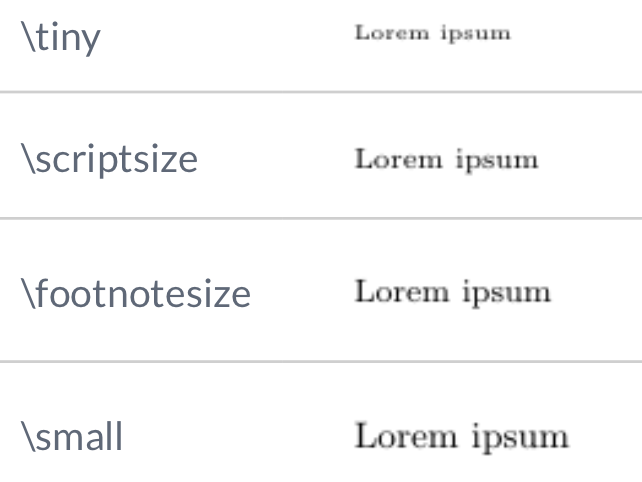
\includegraphics[width=0.5\linewidth]{figures/sample-content/latex_font_sizes} 

}

\caption{Font sizes in LaTeX}\label{fig:latex-font-sizing}
\end{figure}

Puoi usarli per regolare manualmente la dimensione del carattere nel tuo longtable in due passaggi:

\begin{enumerate}
\def\labelenumi{\arabic{enumi}.}
\tightlist
\item
  Avvolgere l'ambiente longtable, ad esempio, in un ambiente \texttt{scriptsize}, sostituendo una stringa nell'output di \texttt{kable}/\texttt{kableExtra}
\item
  Aggiungi gli attributi che fanno capire a R Markdown che la tabella è una tabella (sembra che R li rilasci quando eseguiamo la sostituzione della stringa)
\end{enumerate}

\begin{Shaded}
\begin{Highlighting}[]
\NormalTok{our\_adjusted\_table }\OtherTok{\textless{}{-}}\NormalTok{ a\_long\_table }\SpecialCharTok{\%\textgreater{}\%} 
  \FunctionTok{kable}\NormalTok{(}\AttributeTok{booktabs =} \ConstantTok{TRUE}\NormalTok{, }\AttributeTok{longtable =} \ConstantTok{TRUE}\NormalTok{) }\SpecialCharTok{\%\textgreater{}\%} 
  \FunctionTok{kable\_styling}\NormalTok{(}\AttributeTok{latex\_options =} \StringTok{"repeat\_header"}\NormalTok{) }\SpecialCharTok{\%\textgreater{}\%} 
  \CommentTok{\# wrap the longtable in a tiny environment}
  \FunctionTok{str\_replace}\NormalTok{(}\StringTok{\textquotesingle{}}\SpecialCharTok{\textbackslash{}\textbackslash{}\textbackslash{}\textbackslash{}}\StringTok{begin}\SpecialCharTok{\textbackslash{}\textbackslash{}}\StringTok{\{longtable}\SpecialCharTok{\textbackslash{}\textbackslash{}}\StringTok{\}\textquotesingle{}}\NormalTok{, }
              \StringTok{\textquotesingle{}}\SpecialCharTok{\textbackslash{}\textbackslash{}\textbackslash{}\textbackslash{}}\StringTok{begin}\SpecialCharTok{\textbackslash{}\textbackslash{}}\StringTok{\{scriptsize}\SpecialCharTok{\textbackslash{}\textbackslash{}}\StringTok{\}}\SpecialCharTok{\textbackslash{}n\textbackslash{}\textbackslash{}\textbackslash{}\textbackslash{}}\StringTok{begin}\SpecialCharTok{\textbackslash{}\textbackslash{}}\StringTok{\{longtable}\SpecialCharTok{\textbackslash{}\textbackslash{}}\StringTok{\}\textquotesingle{}}\NormalTok{) }\SpecialCharTok{\%\textgreater{}\%}
  \FunctionTok{str\_replace}\NormalTok{(}\StringTok{\textquotesingle{}}\SpecialCharTok{\textbackslash{}\textbackslash{}\textbackslash{}\textbackslash{}}\StringTok{end}\SpecialCharTok{\textbackslash{}\textbackslash{}}\StringTok{\{longtable}\SpecialCharTok{\textbackslash{}\textbackslash{}}\StringTok{\}\textquotesingle{}}\NormalTok{, }
              \StringTok{\textquotesingle{}}\SpecialCharTok{\textbackslash{}\textbackslash{}\textbackslash{}\textbackslash{}}\StringTok{end}\SpecialCharTok{\textbackslash{}\textbackslash{}}\StringTok{\{longtable}\SpecialCharTok{\textbackslash{}\textbackslash{}}\StringTok{\}}\SpecialCharTok{\textbackslash{}n\textbackslash{}\textbackslash{}\textbackslash{}\textbackslash{}}\StringTok{end}\SpecialCharTok{\textbackslash{}\textbackslash{}}\StringTok{\{scriptsize}\SpecialCharTok{\textbackslash{}\textbackslash{}}\StringTok{\}\textquotesingle{}}\NormalTok{)}

\CommentTok{\#add attributes to make R Markdown treat this as a kable LaTeX table again}
\NormalTok{our\_adjusted\_table }\SpecialCharTok{\%\textgreater{}\%} 
  \FunctionTok{structure}\NormalTok{(}\AttributeTok{format =} \StringTok{"latex"}\NormalTok{, }\AttributeTok{class =} \StringTok{"knitr\_kable"}\NormalTok{)}
\end{Highlighting}
\end{Shaded}

\begin{scriptsize}
\begin{longtable}{lrrrrrrrrrrr}
\toprule
  & mpg & cyl & disp & hp & drat & wt & qsec & vs & am & gear & carb\\
\midrule
\endfirsthead
\multicolumn{12}{@{}l}{\textit{(continued)}}\\
\toprule
  & mpg & cyl & disp & hp & drat & wt & qsec & vs & am & gear & carb\\
\midrule
\endhead

\endfoot
\bottomrule
\endlastfoot
Mazda RX4 & 21.0 & 6 & 160.0 & 110 & 3.90 & 2.620 & 16.46 & 0 & 1 & 4 & 4\\
Mazda RX4 Wag & 21.0 & 6 & 160.0 & 110 & 3.90 & 2.875 & 17.02 & 0 & 1 & 4 & 4\\
Datsun 710 & 22.8 & 4 & 108.0 & 93 & 3.85 & 2.320 & 18.61 & 1 & 1 & 4 & 1\\
Hornet 4 Drive & 21.4 & 6 & 258.0 & 110 & 3.08 & 3.215 & 19.44 & 1 & 0 & 3 & 1\\
Hornet Sportabout & 18.7 & 8 & 360.0 & 175 & 3.15 & 3.440 & 17.02 & 0 & 0 & 3 & 2\\
\addlinespace
Valiant & 18.1 & 6 & 225.0 & 105 & 2.76 & 3.460 & 20.22 & 1 & 0 & 3 & 1\\
Duster 360 & 14.3 & 8 & 360.0 & 245 & 3.21 & 3.570 & 15.84 & 0 & 0 & 3 & 4\\
Merc 240D & 24.4 & 4 & 146.7 & 62 & 3.69 & 3.190 & 20.00 & 1 & 0 & 4 & 2\\
Merc 230 & 22.8 & 4 & 140.8 & 95 & 3.92 & 3.150 & 22.90 & 1 & 0 & 4 & 2\\
Merc 280 & 19.2 & 6 & 167.6 & 123 & 3.92 & 3.440 & 18.30 & 1 & 0 & 4 & 4\\
\addlinespace
Merc 280C & 17.8 & 6 & 167.6 & 123 & 3.92 & 3.440 & 18.90 & 1 & 0 & 4 & 4\\
Merc 450SE & 16.4 & 8 & 275.8 & 180 & 3.07 & 4.070 & 17.40 & 0 & 0 & 3 & 3\\
Merc 450SL & 17.3 & 8 & 275.8 & 180 & 3.07 & 3.730 & 17.60 & 0 & 0 & 3 & 3\\
Merc 450SLC & 15.2 & 8 & 275.8 & 180 & 3.07 & 3.780 & 18.00 & 0 & 0 & 3 & 3\\
Cadillac Fleetwood & 10.4 & 8 & 472.0 & 205 & 2.93 & 5.250 & 17.98 & 0 & 0 & 3 & 4\\
\addlinespace
Lincoln Continental & 10.4 & 8 & 460.0 & 215 & 3.00 & 5.424 & 17.82 & 0 & 0 & 3 & 4\\
Chrysler Imperial & 14.7 & 8 & 440.0 & 230 & 3.23 & 5.345 & 17.42 & 0 & 0 & 3 & 4\\
Fiat 128 & 32.4 & 4 & 78.7 & 66 & 4.08 & 2.200 & 19.47 & 1 & 1 & 4 & 1\\
Honda Civic & 30.4 & 4 & 75.7 & 52 & 4.93 & 1.615 & 18.52 & 1 & 1 & 4 & 2\\
Toyota Corolla & 33.9 & 4 & 71.1 & 65 & 4.22 & 1.835 & 19.90 & 1 & 1 & 4 & 1\\
\addlinespace
Toyota Corona & 21.5 & 4 & 120.1 & 97 & 3.70 & 2.465 & 20.01 & 1 & 0 & 3 & 1\\
Dodge Challenger & 15.5 & 8 & 318.0 & 150 & 2.76 & 3.520 & 16.87 & 0 & 0 & 3 & 2\\
AMC Javelin & 15.2 & 8 & 304.0 & 150 & 3.15 & 3.435 & 17.30 & 0 & 0 & 3 & 2\\
Camaro Z28 & 13.3 & 8 & 350.0 & 245 & 3.73 & 3.840 & 15.41 & 0 & 0 & 3 & 4\\
Pontiac Firebird & 19.2 & 8 & 400.0 & 175 & 3.08 & 3.845 & 17.05 & 0 & 0 & 3 & 2\\
\addlinespace
Fiat X1-9 & 27.3 & 4 & 79.0 & 66 & 4.08 & 1.935 & 18.90 & 1 & 1 & 4 & 1\\
Porsche 914-2 & 26.0 & 4 & 120.3 & 91 & 4.43 & 2.140 & 16.70 & 0 & 1 & 5 & 2\\
Lotus Europa & 30.4 & 4 & 95.1 & 113 & 3.77 & 1.513 & 16.90 & 1 & 1 & 5 & 2\\
Ford Pantera L & 15.8 & 8 & 351.0 & 264 & 4.22 & 3.170 & 14.50 & 0 & 1 & 5 & 4\\
Ferrari Dino & 19.7 & 6 & 145.0 & 175 & 3.62 & 2.770 & 15.50 & 0 & 1 & 5 & 6\\
\addlinespace
Maserati Bora & 15.0 & 8 & 301.0 & 335 & 3.54 & 3.570 & 14.60 & 0 & 1 & 5 & 8\\
Volvo 142E & 21.4 & 4 & 121.0 & 109 & 4.11 & 2.780 & 18.60 & 1 & 1 & 4 & 2\\
Mazda RX41 & 21.0 & 6 & 160.0 & 110 & 3.90 & 2.620 & 16.46 & 0 & 1 & 4 & 4\\
Mazda RX4 Wag1 & 21.0 & 6 & 160.0 & 110 & 3.90 & 2.875 & 17.02 & 0 & 1 & 4 & 4\\
Datsun 7101 & 22.8 & 4 & 108.0 & 93 & 3.85 & 2.320 & 18.61 & 1 & 1 & 4 & 1\\
\addlinespace
Hornet 4 Drive1 & 21.4 & 6 & 258.0 & 110 & 3.08 & 3.215 & 19.44 & 1 & 0 & 3 & 1\\
Hornet Sportabout1 & 18.7 & 8 & 360.0 & 175 & 3.15 & 3.440 & 17.02 & 0 & 0 & 3 & 2\\
Valiant1 & 18.1 & 6 & 225.0 & 105 & 2.76 & 3.460 & 20.22 & 1 & 0 & 3 & 1\\
Duster 3601 & 14.3 & 8 & 360.0 & 245 & 3.21 & 3.570 & 15.84 & 0 & 0 & 3 & 4\\
Merc 240D1 & 24.4 & 4 & 146.7 & 62 & 3.69 & 3.190 & 20.00 & 1 & 0 & 4 & 2\\
\addlinespace
Merc 2301 & 22.8 & 4 & 140.8 & 95 & 3.92 & 3.150 & 22.90 & 1 & 0 & 4 & 2\\
Merc 2801 & 19.2 & 6 & 167.6 & 123 & 3.92 & 3.440 & 18.30 & 1 & 0 & 4 & 4\\
Merc 280C1 & 17.8 & 6 & 167.6 & 123 & 3.92 & 3.440 & 18.90 & 1 & 0 & 4 & 4\\
Merc 450SE1 & 16.4 & 8 & 275.8 & 180 & 3.07 & 4.070 & 17.40 & 0 & 0 & 3 & 3\\
Merc 450SL1 & 17.3 & 8 & 275.8 & 180 & 3.07 & 3.730 & 17.60 & 0 & 0 & 3 & 3\\
\addlinespace
Merc 450SLC1 & 15.2 & 8 & 275.8 & 180 & 3.07 & 3.780 & 18.00 & 0 & 0 & 3 & 3\\
Cadillac Fleetwood1 & 10.4 & 8 & 472.0 & 205 & 2.93 & 5.250 & 17.98 & 0 & 0 & 3 & 4\\
Lincoln Continental1 & 10.4 & 8 & 460.0 & 215 & 3.00 & 5.424 & 17.82 & 0 & 0 & 3 & 4\\
Chrysler Imperial1 & 14.7 & 8 & 440.0 & 230 & 3.23 & 5.345 & 17.42 & 0 & 0 & 3 & 4\\
Fiat 1281 & 32.4 & 4 & 78.7 & 66 & 4.08 & 2.200 & 19.47 & 1 & 1 & 4 & 1\\
\addlinespace
Honda Civic1 & 30.4 & 4 & 75.7 & 52 & 4.93 & 1.615 & 18.52 & 1 & 1 & 4 & 2\\
Toyota Corolla1 & 33.9 & 4 & 71.1 & 65 & 4.22 & 1.835 & 19.90 & 1 & 1 & 4 & 1\\
Toyota Corona1 & 21.5 & 4 & 120.1 & 97 & 3.70 & 2.465 & 20.01 & 1 & 0 & 3 & 1\\
Dodge Challenger1 & 15.5 & 8 & 318.0 & 150 & 2.76 & 3.520 & 16.87 & 0 & 0 & 3 & 2\\
AMC Javelin1 & 15.2 & 8 & 304.0 & 150 & 3.15 & 3.435 & 17.30 & 0 & 0 & 3 & 2\\
\addlinespace
Camaro Z281 & 13.3 & 8 & 350.0 & 245 & 3.73 & 3.840 & 15.41 & 0 & 0 & 3 & 4\\
Pontiac Firebird1 & 19.2 & 8 & 400.0 & 175 & 3.08 & 3.845 & 17.05 & 0 & 0 & 3 & 2\\
Fiat X1-91 & 27.3 & 4 & 79.0 & 66 & 4.08 & 1.935 & 18.90 & 1 & 1 & 4 & 1\\
Porsche 914-21 & 26.0 & 4 & 120.3 & 91 & 4.43 & 2.140 & 16.70 & 0 & 1 & 5 & 2\\
Lotus Europa1 & 30.4 & 4 & 95.1 & 113 & 3.77 & 1.513 & 16.90 & 1 & 1 & 5 & 2\\
\addlinespace
Ford Pantera L1 & 15.8 & 8 & 351.0 & 264 & 4.22 & 3.170 & 14.50 & 0 & 1 & 5 & 4\\
Ferrari Dino1 & 19.7 & 6 & 145.0 & 175 & 3.62 & 2.770 & 15.50 & 0 & 1 & 5 & 6\\
Maserati Bora1 & 15.0 & 8 & 301.0 & 335 & 3.54 & 3.570 & 14.60 & 0 & 1 & 5 & 8\\
Volvo 142E1 & 21.4 & 4 & 121.0 & 109 & 4.11 & 2.780 & 18.60 & 1 & 1 & 4 & 2\\*
\end{longtable}
\end{scriptsize}

\begin{savequote}
There is grandeur in this view of life, with its several powers, having
been originally breathed into a few forms or into one; and that, whilst
this planet has gone cycling on according to the fixed law of gravity,
from so simple a beginning endless forms most beautiful and most
wonderful have been, and are being, evolved.
\qauthor{--- Charles Darwin (\protect\hyperlink{ref-Darwin1859}{Darwin, 1859})}\end{savequote}



\hypertarget{customizzazioni-ed-estensioni}{%
\chapter{Customizzazioni ed estensioni}\label{customizzazioni-ed-estensioni}}

\minitoc 

\noindent Questo capitolo descrive una serie di suggerimenti e trucchi aggiuntivi, nonché possibili personalizzazioni alla tesi di \texttt{cattolicadown}.

\hypertarget{cache-di-chunk-e-la-cartella-_bookdown_files}{%
\section{cache di chunk e la cartella **~\_bookdown\_files**}\label{cache-di-chunk-e-la-cartella-_bookdown_files}}

Se si imposta \texttt{cache\ =\ true} in un blocco di codice, per memorizzare nella memorizzazione la memorizzazione dei risultati se richiede tempo per eseguire, consultare {[}la documentazione R Markdown{]} (\url{https://bookdown.org/yihui/rmarkdown-cookbook/cache}. HTML), quindi i file per la memorizzazione nella cache sono archiviati nella cartella **\_bookdown\_files**.

Se non usi la memorizzazione nella cache e desideri semplicemente avere la cartella ** \_ bookdown\_files ** eliminata dopo il completamento del processo di build, impostare \texttt{abilit\_cache\ =\ false} in \textbf{index.rmd }.

Cioè, il tuo yaml dovrebbe assomigliare a questo:

\begin{Shaded}
\begin{Highlighting}[]
\FunctionTok{knit}\KeywordTok{:}\AttributeTok{ (function(input, ...) \{}
\AttributeTok{    thesis\_formats \textless{}{-} "pdf";}
\AttributeTok{    }
\AttributeTok{    source("scripts\_and\_filters/knit{-}functions.R");}
\AttributeTok{    knit\_thesis(input, thesis\_formats, allow\_cache = FALSE, ...)}
\AttributeTok{  \})}
\end{Highlighting}
\end{Shaded}

\hypertarget{fronte-pagina}{%
\section{Fronte Pagina}\label{fronte-pagina}}

\hypertarget{accorcia-le-didascalie-mostrate-nellelenco-delle-figure-pdf}{%
\subsection{Accorcia le didascalie mostrate nell'elenco delle figure (PDF)}\label{accorcia-le-didascalie-mostrate-nellelenco-delle-figure-pdf}}

Potresti voler che il tuo elenco di cifre (che segue il contenuto del contenuto) abbia descrizioni di figure più brevi (o semplicemente diverse) rispetto alle didascalie alla figura effettiva.

Fallo usando l'opzione chunk \texttt{Fig.scap} (`didascalia breve'), ad esempio\texttt{\{R\ Captain-Image,\ fig.cap\ =\ "Una\ didascalia\ molto\ lunga\ e\ descrittiva\ (e\ potenzialmente\ noiosa)\ che\ non\ si\ adatta\ alla\ Elenco\ delle\ figure,\ ma\ aiuta\ il\ lettore\ a\ capire\ cosa\ comunica\ la\ figura.\ ",\ fig.scap\ ="\ Una\ descrizione\ concisa\ per\ l\textquotesingle{}elenco\ delle\ figure\ "}

\hypertarget{abbrevia-le-didascalie-visualizzate-nellelenco-delle-tabelle-pdf}{%
\subsection{abbrevia le didascalie visualizzate nell'elenco delle tabelle (PDF)}\label{abbrevia-le-didascalie-visualizzate-nellelenco-delle-tabelle-pdf}}

È possibile che l'elenco delle tabelle (che segue l'elenco delle figure nel frontespizio della tesi) abbia descrizioni delle tabelle più brevi (o semplicemente diverse) rispetto alle didascalie delle tabelle stesse.

Se stai usando \texttt{knitr::kable} per generare una tabella, puoi farlo con l'argomento \texttt{caption.short}, ad esempio:

\begin{Shaded}
\begin{Highlighting}[]
\NormalTok{knitr}\SpecialCharTok{::}\FunctionTok{kable}\NormalTok{(mtcars,}
              \AttributeTok{caption =} \StringTok{"Una didascalia molto lunga e descrittiva (e potenzialmente}
\StringTok{               noioso) che non si adatta all\textquotesingle{}elenco delle figure,}
\StringTok{               ma aiuta il lettore a capire cosa la figura}
\StringTok{               comunica."}\NormalTok{,}
              \AttributeTok{caption.short =} \StringTok{"Una descrizione concisa per l\textquotesingle{}elenco delle tabelle"}\NormalTok{)}
\end{Highlighting}
\end{Shaded}

\hypertarget{accorciare-lintestazione-di-corsa-pdf}{%
\section{Accorciare l'intestazione di corsa (PDF)}\label{accorciare-lintestazione-di-corsa-pdf}}

Potresti voler l'intestazione nel mezzo di un capitolo (ovvero l'intestazione che mostra il titolo all'interno dell'attuale capitolo nella parte superiore della pagina) è più breve (o semplicemente diversa) rispetto al titolo del capitolo effettivo.

Fallo aggiungendo il comando latex \texttt{\textbackslash{}\ capitolo\ \{la\ mia\ versione\ più\ corta\}} dopo il titolo del capitolo.

Ad esempio, il capitolo ~(\protect\hyperlink{ref-ref}{\textbf{ref?}}) (cittadini e refs) è semplicemente ``cita e cross-refs'', perché inizia così:

\begin{Shaded}
\begin{Highlighting}[]
\FunctionTok{\# Citations, cross{-}references, and collaboration \{\#cites{-}and{-}refs\} }
\NormalTok{\textbackslash{}chaptermark\{Cites and cross{-}refs\}}
\end{Highlighting}
\end{Shaded}

\hypertarget{capitoli-non-numerati}{%
\section{Capitoli non numerati}\label{capitoli-non-numerati}}

Per rendere i capitoli non numerati (normalmente lo fai per l'introduzione e/o la conclusione), far seguire l'intestazione del capitolo a \texttt{\{-\}}, ad es. \texttt{\#\ Introduzione\ \{-\}}.

Quando lo fai, ricordati che devi anche mettere questi due comandi in LaTeX:

\begin{Shaded}
\begin{Highlighting}[]
\FunctionTok{\textbackslash{}adjustmtc}
\FunctionTok{\textbackslash{}markboth}\NormalTok{\{The Name of Your Unnumbered Chapter\}\{\}}
\end{Highlighting}
\end{Shaded}

Altrimenti il mini-sommario del capitolo e l'intestazione mostreranno il capitolo precedente.

\hypertarget{capitoli-iniziali-con-citazioni-pdf}{%
\section{Capitoli iniziali con citazioni (PDF)}\label{capitoli-iniziali-con-citazioni-pdf}}

Il modello di LaTeX di Oxthesis ti consente di includere anche un blocco di tipo \texttt{savequote} all'inizio dei capitoli.
Per farlo, usa la sintassi \texttt{} \texttt{\{block\ type\ =\ \textquotesingle{}savequote\textquotesingle{}\}} ``.\footnote{Per ulteriori informazioni sui tipi di blocchi personalizzati, consultare la sezione in {[}\emph{authoring libri con r markdown }{]} (https (https : //bookdown.org/yihui/bookdown/custom-blocks.html).}

Aggiungi la referenza della citazione con l'opzione chunk \texttt{quote\_author\ ="\ il\ mio\ nome\ autore\ "}.
Ti consiglio anche di aggiungere l'opzione chunk \texttt{include\ =\ knitr::is\_latex\_output()} in modo che le citazioni siano incluse solo nell'output PDF.

Non è possibile utilizzare la sintassi di Markdown all'interno delle opzioni di chunk, quindi se si desidera ad es. in corsivo un nome del libro usa \href{https://bookdown.org/yihui/Bookdown/markdown-extensions-by-Bookdown.html\#text-references}{`Testo Reference'}: crea un pezzo di testo chiamato con `(rif: etichetta) il mio testo', quindi indica questo nell'opzione chunk con \texttt{quote\_author\ =\ \textquotesingle{}(rif:\ etichetta)\textquotesingle{}}.

\hypertarget{evidenziazione-delle-correzioni-html-e-pdf}{%
\section{Evidenziazione delle correzioni (HTML e PDF)}\label{evidenziazione-delle-correzioni-html-e-pdf}}

Quando arriva il momento di fare correzioni, potresti voler evidenziare le modifiche apportate corretta agli esaminatori in modo che possano verificare rapidamente di le cose cambiate
Puoi farlo così:

\hypertarget{correzioni-in-linea-brevi}{%
\subsection{correzioni in linea brevi}\label{correzioni-in-linea-brevi}}

Evidenzia \textbf{correzioni brevi e inline } facendo \texttt{{[}come\ questo{]}\ \{.correction\}} --- Il testo tra le parentesi quadrate verrà quindi \hl{evidenziato in blu} nell'output.

Si noti che Pandoc potrebbe essere confuso da citazioni e riferimenti incrociati all'interno delle correzioni in linea.
In particolare, potrebbe essere confuso da \texttt{"\ {[}cosa\ ha\ detto\ @shea2014{]}\ \{.correction\}\ "} che diventa (cosa ha detto \protect\hyperlink{ref-shea2014}{\textbf{shea2014?}}) \{. Correzione\}
In tali casi, è possibile utilizzare direttamente la sintassi in lattice.
L'evidenziazione della correzione usa il pacchetto {[}Soul{]} (\url{https://ctan.org/pkg/soul}), quindi puoi fare così:

\begin{itemize}
\tightlist
\item
  Se si utilizza BiBLATEX per i riferimenti, usa `~hl \{What ~textCite \{Shea2014\} detto\}\}
\item
  Se si utilizza Natbib per riferimenti, usa `~hl \{cosa ~cite \{shea2014\} detto\}\}
\end{itemize}

L'uso di LaTeX grezzo ha lo svantaggio delle correzioni, quindi non viene visualizzata nell'output HTML, ma potresti comunque preoccuparti dell'evidenziazione della correzione nel PDF per gli esaminatori!

\hypertarget{blocchi-di-materiale-aggiunto-o-modificato}{%
\subsection{blocchi di materiale aggiunto o modificato}\label{blocchi-di-materiale-aggiunto-o-modificato}}

Evidenzia interi ** blocchi di materiale aggiunto o modificato ** mettendoli in un blocco di tipo \texttt{correzione}, usando la sintassi\texttt{\textasciigrave{}\textasciigrave{}\ \textasciigrave{}\textasciigrave{}}\{Block type = `correction'\}\texttt{\textasciigrave{}\textasciigrave{}.\^{}{[}In\ Il\ file\ **.\ tex\ **\ per\ output\ PDF,\ questo\ metterà\ il\ contenuto\ tra}~inizio \{correzione\}\texttt{e}~end \{correzione\}\texttt{;\ Nell\textquotesingle{}output\ di\ GitBook\ sarà\ messo\ tra}

\texttt{e}

`.{]}
Così:

\begin{correction}
Per blocchi più grandi, come questo paragrafo o addirittura intere
figure, è possibile utilizzare il tipo di blocco ``Correction''. Questo
ambiente \textbf{mette in evidenza blocchi di dimensioni del paragrafo e
più grandi} con lo stesso colore blu.
\end{correction}

\emph{Si noti che i blocchi di correzione non possono essere inclusi nell'output delle parole.}

\hypertarget{che-interrompe-le-correzioni-da-essere-evidenziate}{%
\subsection{che interrompe le correzioni da essere evidenziate}\label{che-interrompe-le-correzioni-da-essere-evidenziate}}

Per disattivare l'evidenziazione della correzione, vai all'intestazione YAML di ** INDICE.RMD **, quindi:

\begin{itemize}
\tightlist
\item
  Output PDF: Imposta \texttt{Correzioni:\ False}\\
\item
  output HTML: rimuovi o commenta \texttt{-\ modelli/corrections.css}
\end{itemize}

\hypertarget{applicare-il-colore-del-carattere-personalizzato-ed-evidenziazione-a-testo-html-e-pdf}{%
\section{Applicare il colore del carattere personalizzato ed evidenziazione a testo (HTML e PDF)}\label{applicare-il-colore-del-carattere-personalizzato-ed-evidenziazione-a-testo-html-e-pdf}}

Il filtro LUA che aggiunge la funzionalità per evidenziare le correzioni aggiunge altri due trucchi:
Puoi applicare la tua scelta di colore per evidenziare il testo o cambiare il colore del carattere.
La sintassi è la seguente:

\begin{quote}
Ecco \texttt{{[}qualche\ testo\ in\ posa\ evidenziazione{]}\ \{evidenziazione\ ="\ rosa\ "\}}\\
Diventa: ecco {[}alcuni testi in evidenza rosa{]} \{evidenziazione = ``rosa''\}.
\end{quote}

\begin{quote}
\texttt{{[}Ecco\ un\ po\ \textquotesingle{}di\ testo\ con\ font\ blu{]}\ \{color\ ="\ blu\ "\}}\strut \\
Diventa: {[}Ecco un po 'di testo con font blu{]} \{color = ``blu''\}
\end{quote}

\begin{quote}
Finalmente --- Mai e poi mai in realtà questo-\texttt{{[}Ecco\ un\ po\ \textquotesingle{}di\ testo\ con\ evidenziazione\ nera\ e\ carattere\ giallo{]}\ \{evidenziazione\ ="\ nero\ "color\ ="\ giallo\ "\}}\\
Diventa: {[}Ecco un po 'di testo con evidenziazione nera e carattere giallo{]} \{evidenziazione = ``nero'' color = ``giallo''\}
\end{quote}

Il file ** Scripts\_and\_filters/Colour\_and\_highlight.lua ** implementa questo, se si desidera armeggiare con esso.
Funziona con output PDF e HTML.

\hypertarget{aggiunta-di-un-secondo-astratto-pdf}{%
\section{Aggiunta di un secondo astratto (PDF)}\label{aggiunta-di-un-secondo-astratto-pdf}}

Potresti aver bisogno di due abstract nella tua tesi, se ad es. Ho bisogno sia di un astratto in inglese che di qualche altra lingua.

Puoi aggiungere un secondo abstract in ** index.rmd ** come: così:

\begin{Shaded}
\begin{Highlighting}[]
\FunctionTok{abstract{-}second{-}heading}\KeywordTok{:}\AttributeTok{ }\StringTok{"Resumé"}
\FunctionTok{abstract{-}second}\KeywordTok{:}\AttributeTok{ }\StringTok{"This is the second abstract, for example in beautiful French."}\AttributeTok{ }
\end{Highlighting}
\end{Shaded}

\hypertarget{incluso-un-altro-documento-nella-tesi---incorporare-un-documento-pdf-embed--pdf}{%
\section{incluso un altro documento nella tesi - Incorporare un documento PDF \{\#embed -pdf\}}\label{incluso-un-altro-documento-nella-tesi---incorporare-un-documento-pdf-embed--pdf}}

Potresti voler incorporare documenti PDF esistenti nella tesi, ad esempio se il tuo dipartimento consente una tesi di stile ``Portfolio'' e devi includere una pubblicazione di composizione esistente come capitolo.

Nell'output di GitBook, puoi semplicemente usare \texttt{Knitr\ ::\ Include\_Graphics} e dovrebbe includere un PDF scorrevole (e scaricabile).
Probabilmente vorrai impostare le opzioni di chunk \texttt{out.width\ =\ \textquotesingle{}100\%\textquotesingle{}} e \texttt{out.height\ =\ \textquotesingle{}1000px\textquotesingle{}}:

\begin{Shaded}
\begin{Highlighting}[]
\NormalTok{knitr}\SpecialCharTok{::}\FunctionTok{include\_graphics}\NormalTok{(}\StringTok{"figures/sample{-}content/pdf\_embed\_example/Lyngs2020\_FB.pdf"}\NormalTok{)}
\end{Highlighting}
\end{Shaded}

Nell'output in lattice, tuttavia, questo approccio può causare comportamenti strani.
Pertanto, quando si crea la tesi su PDF, dividere il PDF in una sequenza alfanumericamente ordinata di ** file pdf ** a pagina singola ** (puoi farlo automaticamente con il pacchetto \texttt{pdftools}). È quindi possibile utilizzare il comando in lattice appropriato per inserirli, come mostrato di seguito (per brevità, nel contenuto di esempio di \texttt{Oxforddown} PDF stiamo includendo solo due pagine).
\emph{Si noti che l'opzione chunk \texttt{risultati\ =\ \textquotesingle{}asis\textquotesingle{}} deve essere impostata.}
È inoltre possibile rimuovere i margini dai file PDF, che puoi fare con Adobe Acrobat (versione a pagamento) e probabilmente altri software.

\begin{Shaded}
\begin{Highlighting}[]
\CommentTok{\# install.packages(pdftools)}
\CommentTok{\# split PDF into pages stored in}
\NormalTok{    figures}\SpecialCharTok{/}\NormalTok{sample}\SpecialCharTok{{-}}\NormalTok{content}\SpecialCharTok{/}\NormalTok{pdf\_embed\_example}\SpecialCharTok{/}\NormalTok{split}\SpecialCharTok{/}
\CommentTok{\#}
\NormalTok{    pdftools}\SpecialCharTok{::}\FunctionTok{pdf\_split}\NormalTok{(}\StringTok{"figures/sample{-}content/pdf\_embed\_example/Lyngs2020\_FB.pdf"}\NormalTok{,}
\CommentTok{\# output = "figures/sample{-}content/pdf\_embed\_example/split/")}

\CommentTok{\# grab the pages}
\NormalTok{pages }\OtherTok{\textless{}{-}} \FunctionTok{list.files}\NormalTok{(}\StringTok{"figures/sample{-}content/pdf\_embed\_example/split"}\NormalTok{,}
    \AttributeTok{full.names =} \ConstantTok{TRUE}\NormalTok{)}

\CommentTok{\# set how wide you want the inserted PDFs to be:}
\CommentTok{\# 1.0 is 100 per cent of the oxforddown PDF page width;}
\CommentTok{\# you may want to make it a bit bigger}
\NormalTok{pdf\_width }\OtherTok{\textless{}{-}} \FloatTok{1.2}

\CommentTok{\# for each PDF page, insert it nicely and}
\CommentTok{\# end with a page break}
\FunctionTok{cat}\NormalTok{(stringr}\SpecialCharTok{::}\FunctionTok{str\_c}\NormalTok{(}\StringTok{"}\SpecialCharTok{\textbackslash{}\textbackslash{}}\StringTok{newpage }\SpecialCharTok{\textbackslash{}\textbackslash{}}\StringTok{begin\{center\}}
\StringTok{    }\SpecialCharTok{\textbackslash{}\textbackslash{}}\StringTok{makebox[}\SpecialCharTok{\textbackslash{}\textbackslash{}}\StringTok{linewidth][c]\{}\SpecialCharTok{\textbackslash{}\textbackslash{}}\StringTok{includegraphics[width="}\NormalTok{, pdf\_width,}
    \StringTok{"}\SpecialCharTok{\textbackslash{}\textbackslash{}}\StringTok{linewidth]\{"}\NormalTok{, pages, }\StringTok{"\}\} }\SpecialCharTok{\textbackslash{}\textbackslash{}}\StringTok{end\{center\}"}\NormalTok{))}
\end{Highlighting}
\end{Shaded}

\newpage \begin{center} \makebox[\linewidth][c]{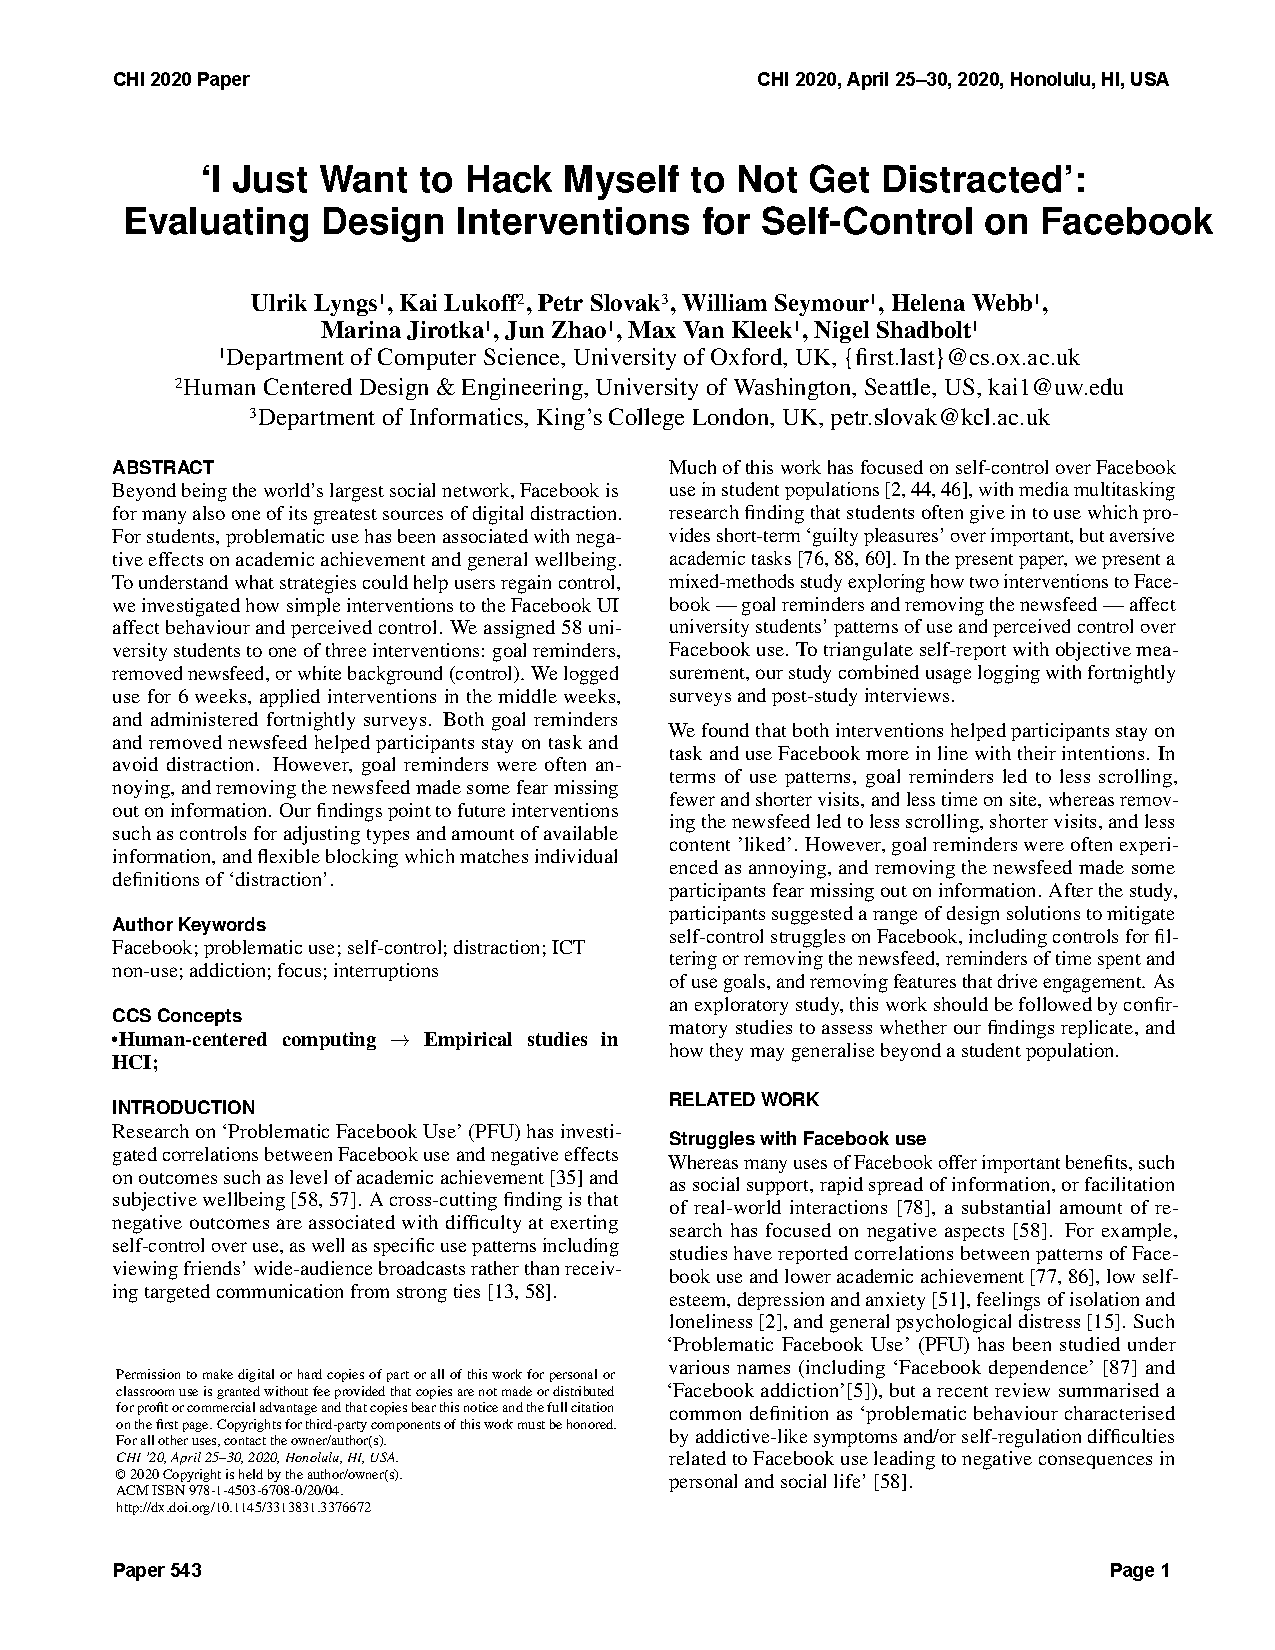
\includegraphics[width=1.2\linewidth]{figures/sample-content/pdf_embed_example/split/_000000000000001.pdf}} \end{center} \newpage \begin{center} \makebox[\linewidth][c]{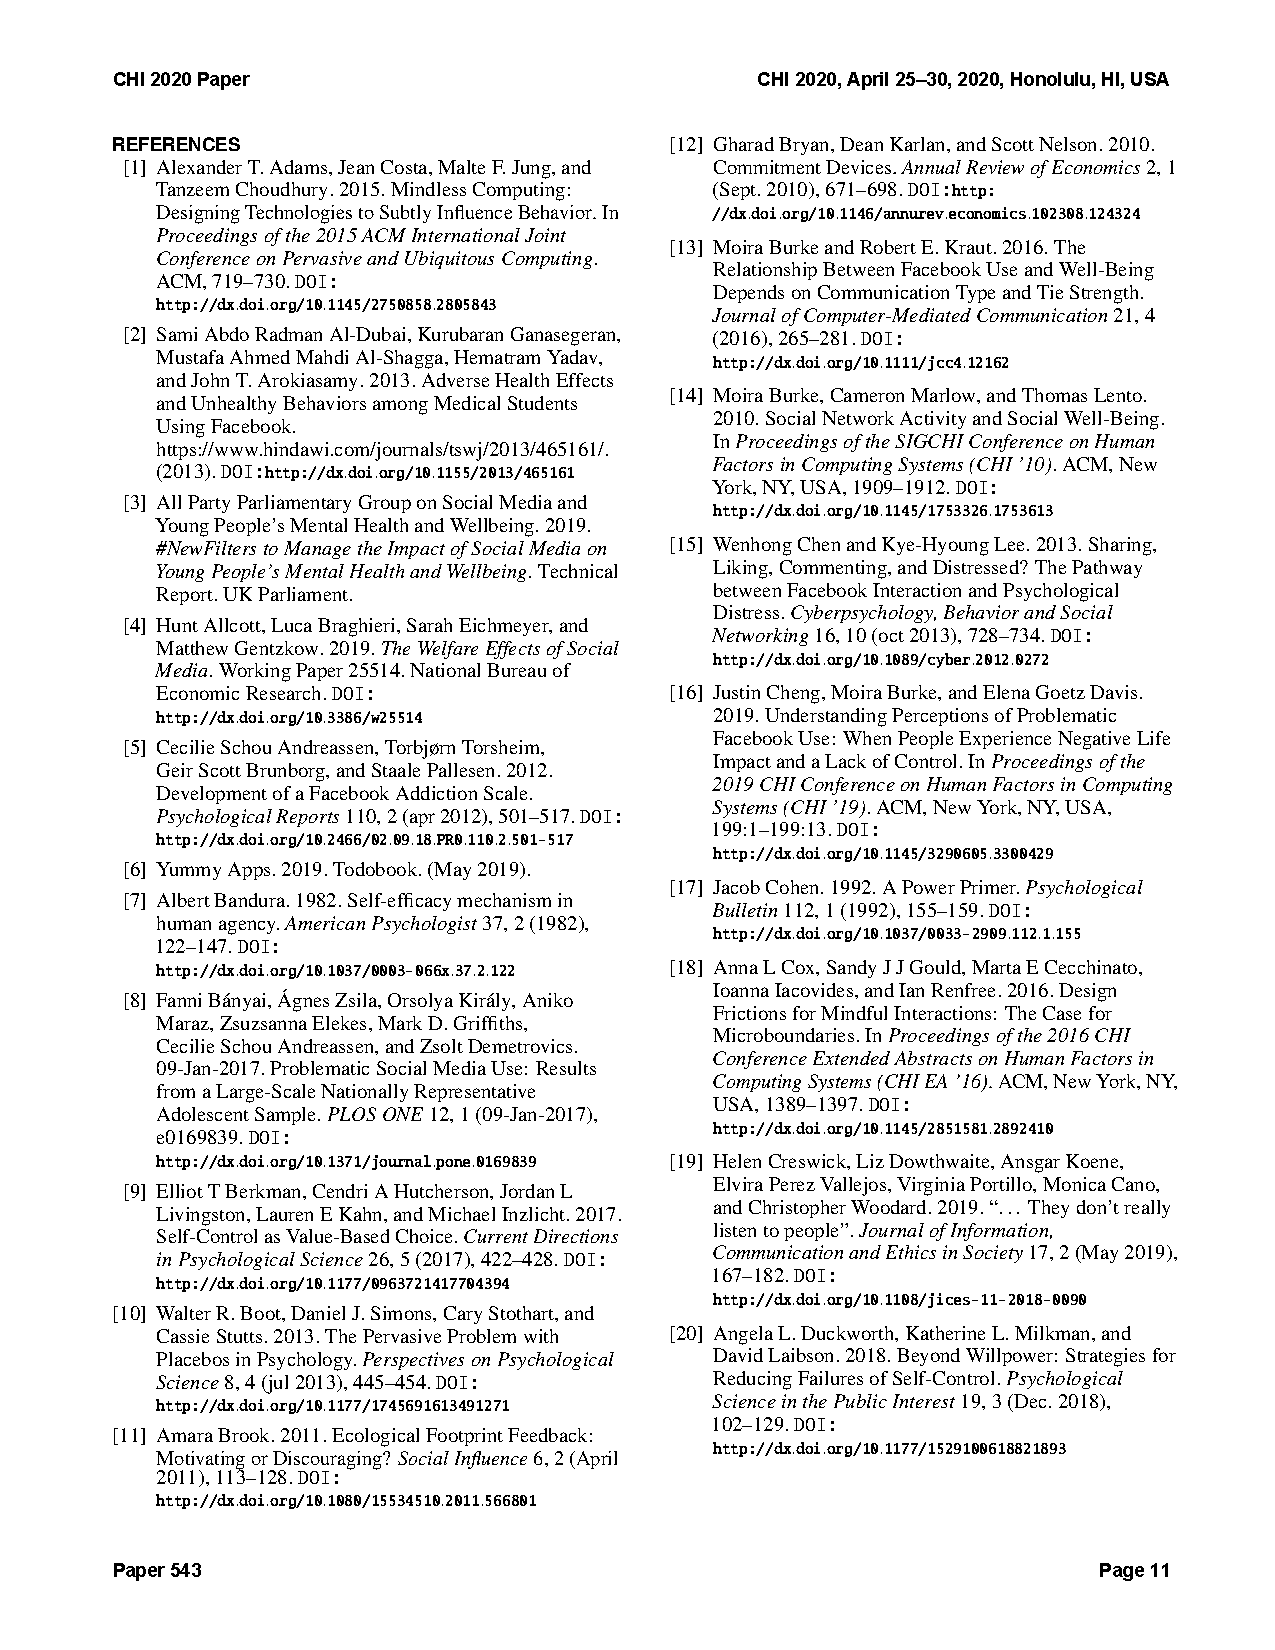
\includegraphics[width=1.2\linewidth]{figures/sample-content/pdf_embed_example/split/_000000000000011.pdf}} \end{center}

\hypertarget{incluso-un-altro-documento-nella-tesi---r-documento-figlio-markdown-embed--rmd}{%
\section{incluso un altro documento nella tesi - r documento figlio markdown \{\#embed -rmd\}}\label{incluso-un-altro-documento-nella-tesi---r-documento-figlio-markdown-embed--rmd}}

A volte vuoi includere un altro documento che stai attualmente scrivendo come capitolo della tua tesi.
Sopra ~(\protect\hyperlink{ref-ref}{\textbf{ref?}}) (embed-pdf), abbiamo descritto il modo più semplice per farlo: includere l'altro documento come PDF.
Tuttavia, in alcuni casi invece si desidera includere la sorgente di markdown R da questo documento e farlo compilare all'interno della tesi.
Questo è un po 'più complicato, perché è necessario tenere traccia attenta dei percorsi dei file, ma è possibile tramite {[}incluso il documento di un bambino{]} (\url{https://bookdown.org/yihui/rmarkdown-cookbook/child} -Document.html).
Ci sono quattro passaggi principali:

\begin{enumerate}
\def\labelenumi{\arabic{enumi}.}
\tightlist
\item
  Includi il documento di carta come bambino
\item
  Rendi i percorsi di file compatibili con il lavoro a maglia l'articolo da solo, nonché quando include nella tesi
\item
  Rendi corretti i livelli di intestazione
\item
  Rendi corretti le larghezze della figura
\end{enumerate}

\hypertarget{un-documento-di-esempio-in-unaltra-cartella}{%
\subsection{Un documento di esempio in un'altra cartella}\label{un-documento-di-esempio-in-unaltra-cartella}}

Prendi questo semplice esempio (i file per questo sono in {[}questo repository github{]} (\url{https://github.com/ulyngs/oxforddown-external-article})):

\begin{Shaded}
\begin{Highlighting}[]
\NormalTok{|{-}{-}paper\_to\_include}
\NormalTok{|  |{-}{-}my\_paper.Rmd}
\NormalTok{|  |{-}{-}data}
\NormalTok{|  |  |{-}{-}cat\_salt.csv}
\NormalTok{|  |{-}{-}figures}
\NormalTok{|  |  |{-}{-}cat.jpg}
\NormalTok{|}
\NormalTok{|{-}{-}thesis}
\end{Highlighting}
\end{Shaded}

Come suggerisce il grafico, hai un'altra cartella, ** Paper\_to\_include/** che vive nella stessa cartella contenente della cartella di tesi.
Nella cartella ** paper\_to\_include \textbf{, il file } my\_paper.rmd ** è dove scrivi la carta.
In ** my\_paper.rmd \textbf{, hai letto in un file CSV che si trova nella sottocartella } Data/Cats.csv ** e anche un'immagine della sottocartella ** Figures/Cat.jpg **.

\hypertarget{passaggio-1-includere-la-carta-come-documento-figlio}{%
\subsection{PASSAGGIO 1: includere la carta come documento figlio}\label{passaggio-1-includere-la-carta-come-documento-figlio}}

Nella cartella di tesi, crea un file RMD per il capitolo in cui si desidera includere un altro documento.
Aggiungi uno o più blocchi di codice che includono i file di markdown r da quel documento come documenti figlio:

\begin{Shaded}
\begin{Highlighting}[]
\FunctionTok{\# Including an external chapter }

\InformationTok{\textasciigrave{}\textasciigrave{}\textasciigrave{}\{r child = "../paper\_to\_include/my\_paper.Rmd"\}}
\InformationTok{\textasciigrave{}\textasciigrave{}\textasciigrave{}}
\end{Highlighting}
\end{Shaded}

\hypertarget{passaggio-2-rendi-compatibili-percorsi-di-file}{%
\subsection{Passaggio 2: Rendi compatibili percorsi di file}\label{passaggio-2-rendi-compatibili-percorsi-di-file}}

Utilizzare {[}Parametri{]} (\url{https://rmarkdown.studio.com/lesson-6.html}) per regolare il percorso del file delle immagini in base ai valori impostati nell'intestazione YAML di un file di markdown R.
In ** my\_paper.rmd **, crea un parametro chiamato \texttt{altro\_path} e impostalo su una stringa vuota:

\begin{Shaded}
\begin{Highlighting}[]
\PreprocessorTok{{-}{-}{-}}
\FunctionTok{title}\KeywordTok{:}\AttributeTok{ }\StringTok{"A fabulous article in a different folder"}
\FunctionTok{params}\KeywordTok{:}
\AttributeTok{  }\FunctionTok{other\_path}\KeywordTok{:}\AttributeTok{ }\StringTok{""}
\PreprocessorTok{{-}{-}{-}}
\end{Highlighting}
\end{Shaded}

In ** my\_paper.rmd **, mettilo all'inizio di FilePath quando leggi i dati o includi immagini:

\begin{Shaded}
\begin{Highlighting}[]
\FunctionTok{library}\NormalTok{(tidyverse)}
\FunctionTok{library}\NormalTok{(knitr)}

\NormalTok{cat\_data }\OtherTok{\textless{}{-}} \FunctionTok{read\_csv}\NormalTok{(}\FunctionTok{str\_c}\NormalTok{(params}\SpecialCharTok{$}\NormalTok{other\_path, }\StringTok{"data/cats.csv"}\NormalTok{))}
\FunctionTok{include\_graphics}\NormalTok{(}\FunctionTok{str\_c}\NormalTok{(params}\SpecialCharTok{$}\NormalTok{other\_path, }\StringTok{"figures/cat.jpg"}\NormalTok{))}
\end{Highlighting}
\end{Shaded}

Infine, nel file ** indice.rmd ** della cartella tesi, crea anche il parametro \texttt{Altro\_Path}.
Ma qui, impostalo su dove la cartella ** paper\_to\_include/** è relativa alla cartella di tesi:

\begin{Shaded}
\begin{Highlighting}[]
\FunctionTok{params}\KeywordTok{:}
\AttributeTok{  }\FunctionTok{other\_path}\KeywordTok{:}\AttributeTok{ }\StringTok{"../paper\_to\_include/"}
\end{Highlighting}
\end{Shaded}

\hypertarget{nota-sulloutput-html}{%
\subsection{NOTA sull'output HTML}\label{nota-sulloutput-html}}

Nota che se si desidera ospitare una versione HTML sulla tesi online, dovrai includere la grafica nel contenuto che ospiti online - Internet ovviamente non sarà in grado di vedere i filepath che si riferiscono a cose in un'altra cartella il tuo computer!

\hypertarget{passaggio-3-assicurarsi-che-i-livelli-di-intestazione-siano-corretti}{%
\subsection{Passaggio 3: assicurarsi che i livelli di intestazione siano corretti}\label{passaggio-3-assicurarsi-che-i-livelli-di-intestazione-siano-corretti}}

A meno che il documento che desideri includere non sia anche scritto come libro, probabilmente i livelli di intestazione saranno fuori.
Cioè, le intestazioni di livello 1 (\# alcune intestazioni) che usi per le sezioni principali nell'altra carta si trasformano in titoli di accompagnatore se incluse nella tesi.

Per evitare questo, prima \emph{increment tutti i livelli di intestazione di uno in ** paper\_to\_include/my\_paper.rmd ** } (\# qualche intestazione -\textgreater{} \# \# Qualche intestazione).
Quindi in ** paper\_to\_include/** Crea un {[}filtro Lua{]} (\url{https://bookdown.org/yihui/rmarkdown-cookbook/lua-fiterters.html\#lua-filters}) che riduce i livelli di intestazione di uno: creare un file di testo , salvalo come ** ridotto\_header\_level.lua ** e dargli il contenuto di seguito.

\begin{Shaded}
\begin{Highlighting}[]
\KeywordTok{function}\NormalTok{ Header}\OperatorTok{(}\NormalTok{el}\OperatorTok{)}
  \ControlFlowTok{if} \OperatorTok{(}\NormalTok{el}\OperatorTok{.}\NormalTok{level }\OperatorTok{\textless{}=} \DecValTok{1}\OperatorTok{)} \ControlFlowTok{then}
    \FunctionTok{error}\OperatorTok{(}\StringTok{"I don\textquotesingle{}t know how to decrease the level of h1"}\OperatorTok{)}
  \ControlFlowTok{end}
\NormalTok{  el}\OperatorTok{.}\NormalTok{level }\OperatorTok{=}\NormalTok{ el}\OperatorTok{.}\NormalTok{level }\OperatorTok{{-}} \DecValTok{1}
  \ControlFlowTok{return}\NormalTok{ el}
\KeywordTok{end}
\end{Highlighting}
\end{Shaded}

Nell'intestazione Yaml di ** Paper\_to\_include/my\_paper.rmd **, usa questo filtro:

\begin{Shaded}
\begin{Highlighting}[]
\PreprocessorTok{{-}{-}{-}}
\FunctionTok{title}\KeywordTok{:}\AttributeTok{ }\StringTok{"A fabulous article in a different folder"}
\FunctionTok{params}\KeywordTok{:}
\AttributeTok{  }\FunctionTok{other\_path}\KeywordTok{:}\AttributeTok{ }\StringTok{""}
\FunctionTok{output}\KeywordTok{:}
\AttributeTok{  }\FunctionTok{pdf\_document}\KeywordTok{:}\AttributeTok{ }
\AttributeTok{    }\FunctionTok{pandoc\_args}\KeywordTok{:}\AttributeTok{ }\KeywordTok{[}\StringTok{"{-}{-}lua{-}filter=reduce\_header\_level.lua"}\KeywordTok{]}
\PreprocessorTok{{-}{-}{-}}
\end{Highlighting}
\end{Shaded}

Ora, i livelli di intestazione saranno corretti sia quando si lavora da sola e quando è incluso nella tesi.

Nota: potrebbe non essere necessario utilizzare un filtro LUA per spostare l'intestazione-Sembra che potresti semplicemente usare \texttt{Pandoc\_args:\ {[}"-Shift-Heading-level-by\ =\ -1\ "{]}} (vedi https: // pandoc. org/manual.html\#lettore-opzioni)

\hypertarget{passaggio-4.-assicurarsi-che-le-larghezze-della-figura-siano-corrette}{%
\subsection{Passaggio 4. Assicurarsi che le larghezze della figura siano corrette}\label{passaggio-4.-assicurarsi-che-le-larghezze-della-figura-siano-corrette}}

Potrebbe essere che le larghezze della tua figura quando si lavorano a maglia da sola e, quando lo includi nella tesi, debbano essere diversi.
È possibile utilizzare nuovamente i parametri per impostare le larghezze delle figure.

Immagina di volere che la larghezza della figura sia l'80\% della larghezza della pagina quando si lavora da sola, ma al 100\% nella tesi.
In ** paper\_to\_include/my\_paper.rmd **, prima aggiungi un parametro che potremmo chiamare \texttt{out\_width} e impostarlo sulla stringa'' 80\%``:

\begin{Shaded}
\begin{Highlighting}[]
\PreprocessorTok{{-}{-}{-}}
\FunctionTok{title}\KeywordTok{:}\AttributeTok{ }\StringTok{"A fabulous article in a different folder"}
\FunctionTok{params}\KeywordTok{:}
\AttributeTok{  }\FunctionTok{other\_path}\KeywordTok{:}\AttributeTok{ }\StringTok{""}
\AttributeTok{  }\FunctionTok{out\_width}\KeywordTok{:}\AttributeTok{ }\StringTok{"80\%"}
\FunctionTok{output}\KeywordTok{:}
\AttributeTok{  }\FunctionTok{pdf\_document}\KeywordTok{:}\AttributeTok{ }
\AttributeTok{    }\FunctionTok{pandoc\_args}\KeywordTok{:}\AttributeTok{ }\KeywordTok{[}\StringTok{"{-}{-}lua{-}filter=reduce\_header\_level.lua"}\KeywordTok{]}
\PreprocessorTok{{-}{-}{-}}
\end{Highlighting}
\end{Shaded}

Quindi, assicurati di utilizzare quel parametro per impostare la larghezza dell'uscita quando si includono le figure in ** paper\_to\_include/my\_paper.rmd **:

\begin{Shaded}
\begin{Highlighting}[]
\InformationTok{\textasciigrave{}\textasciigrave{}\textasciigrave{}\{r, out.width=params$out\_width, fig.cap="A very funny cat"\}}
\InformationTok{include\_graphics(str\_c(params$other\_path, "figures/cat.jpg"))}
\InformationTok{\textasciigrave{}\textasciigrave{}\textasciigrave{}}
\end{Highlighting}
\end{Shaded}

Infine, crea il parametro \texttt{out\_width} nella tua tesi '** indice.rmd ** File:

\begin{Shaded}
\begin{Highlighting}[]
\FunctionTok{params}\KeywordTok{:}
\AttributeTok{  }\FunctionTok{other\_path}\KeywordTok{:}\AttributeTok{ }\StringTok{"../paper\_to\_include/"}
\AttributeTok{  }\FunctionTok{out\_width}\KeywordTok{:}\AttributeTok{ }\StringTok{"80\%"}
\end{Highlighting}
\end{Shaded}

Ora, la larghezza di output della tua cifra sarà dell'80\% quando si è a maglia il tuo documento da solo e al 100\% quando lo fa a lavorare come documento per bambini della tesi.

\hypertarget{customising-citations}{%
\section{Personalizzazione di citazioni e riferimenti}\label{customising-citations}}

\hypertarget{utilizzo-di-un-file-.csl-con-pandoc}{%
\subsection{Utilizzo di un file .csl con pandoc}\label{utilizzo-di-un-file-.csl-con-pandoc}}

Vedere la sezione \ref{citazione-aspetto}.

L'unico svantaggio di lasciare che pandoc gestisca le citazioni è che (i) non supporta le bibliografie dei capitoli, (ii) se sei un veterano di LaTeX, potresti essere più a tuo agio con \texttt{bilatex} o \texttt{natbib}.

\hypertarget{bilatex-custom}{%
\subsection{\texorpdfstring{Utilizzo di \texttt{bilatex}}{Utilizzo di bilatex}}\label{bilatex-custom}}

Per utilizzare \href{https://www.overleaf.com/learn/latex/Bibliography_management_with_biblatex}{biblatex} per gestire le citazioni, prima decommenta questo in \textbf{index.Rmd}, YAML header:

\begin{Shaded}
\begin{Highlighting}[]
\AnnotationTok{use{-}biblatex:}\CommentTok{ true}
\AnnotationTok{bib{-}latex{-}options:}\CommentTok{ "style=authoryear, sorting=nyt, backend=biber, maxcitenames=2, useprefix, doi=true, isbn=false, uniquename=false"}
\end{Highlighting}
\end{Shaded}

Quindi dì a R Markdown di usare \texttt{biblatex} quando inserisci le citazioni, impostando \texttt{citation\_package:\ biblatex}:

\begin{Shaded}
\begin{Highlighting}[]
\AnnotationTok{output:}
\NormalTok{  bookdown::pdf\_book:}
\NormalTok{    citation\_package: biblatex}
\end{Highlighting}
\end{Shaded}

Per personalizzare l'aspetto delle citazioni, cambia \texttt{bib-latex-options}. Ad esempio, per ottenere \textbf{citazioni numeriche}, con riferimenti in ordine di apparizione nel testo, impostarlo su

\begin{Shaded}
\begin{Highlighting}[]
\AnnotationTok{bib{-}latex{-}options:}\CommentTok{ "style=numeric{-}comp, sorting=none, backend=biber, maxcitenames=2, useprefix, doi=true, isbn=false, uniquename=false"}
\end{Highlighting}
\end{Shaded}

\hypertarget{aggiunta-di-bibliografie-di-capitoli}{%
\subsubsection{Aggiunta di bibliografie di capitoli}\label{aggiunta-di-bibliografie-di-capitoli}}

Se desideri bibliografie di capitoli, prima aggiungi ``refsection=chapter'' alle opzioni biblatex, ad esempio in questo modo:

\begin{Shaded}
\begin{Highlighting}[]
\AnnotationTok{bib{-}latex{-}options:}\CommentTok{ "refsection=chapter, style=authoryear, sorting=nyt, backend=biber, maxcitenames=2, useprefix, doi=true, isbn=false, uniquename=false"}
\end{Highlighting}
\end{Shaded}

In secondo luogo, imposta il parametro \texttt{insertHeadingInPDF:\ false} in \textbf{index.Rmd}, per eliminare l'inclusione di un'intestazione `Riferimenti' alla fine della tesi.

\begin{Shaded}
\begin{Highlighting}[]
\AnnotationTok{params:}
\NormalTok{  insertHeadingInPDF: false}
\end{Highlighting}
\end{Shaded}

Infine inserisci questa riga alla fine di ogni capitolo, per stamparvi le bibliografie:

\begin{Shaded}
\begin{Highlighting}[]
\FunctionTok{\textbackslash{}printbibliography}\NormalTok{[segment=}\FunctionTok{\textbackslash{}therefsection}\NormalTok{,heading=subbibliography]}
\end{Highlighting}
\end{Shaded}

\hypertarget{natbib-custom}{%
\subsection{\texorpdfstring{Utilizzo di \texttt{natbib}}{Utilizzo di natbib}}\label{natbib-custom}}

Per utilizzare \href{https://www.overleaf.com/learn/latex/Bibliography_management_with_natbib}{natbib} per gestire le citazioni, prima decommenta questo in \textbf{index.Rmd}, YAML header:

\begin{Shaded}
\begin{Highlighting}[]
\AnnotationTok{use{-}natbib:}\CommentTok{ true}
\AnnotationTok{natbib{-}citation{-}style:}\CommentTok{ authoryear \#for science, you might want numbers,square}
\AnnotationTok{natbib{-}bibliography{-}style:}\CommentTok{ templates/ACM{-}Reference{-}Format.bst \#e.g. "plainnat", unsrtnat, or path to a .bst file}
\end{Highlighting}
\end{Shaded}

Quindi dì a R Markdown di usare \texttt{natbib} quando inserisci le citazioni, impostando \texttt{citation\_package:\ natbib}:

\begin{Shaded}
\begin{Highlighting}[]
\AnnotationTok{output:}
\NormalTok{  bookdown::pdf\_book:}
\NormalTok{    citation\_package: natbib}
\end{Highlighting}
\end{Shaded}

Per personalizzare l'aspetto delle citazioni, cambia il file \textbf{.bst} a cui punti in \texttt{natbib-bibliography-style}.

\hypertarget{customizing-the-page-headers-and-footers-pdf}{%
\section{Customizing the page headers and footers (PDF)}\label{customizing-the-page-headers-and-footers-pdf}}

\hypertarget{personalizzazione-delle-intestazioni-e-dei-piuxe8-di-pagina-di-pagina-pdf}{%
\section{Personalizzazione delle intestazioni e dei piè di pagina di pagina (PDF)}\label{personalizzazione-delle-intestazioni-e-dei-piuxe8-di-pagina-di-pagina-pdf}}

Questo può ora essere fatto direttamente nell'intestazione YAML di ** Index.rmd \textbf{.
Se sei un esperto di lattice e hai bisogno di ulteriore personalizzazione che ciò che è attualmente fornito, è possibile modificare le sezioni pertinenti di } modelli/template.tex ** - Il codice pertinente è sotto la linea che inizia \texttt{\textbackslash{}\ usepackage\ \{FancyHdr\}}.

\hypertarget{immergersi-nel-modello-di-lattice-di-oxthesis-pdf}{%
\section{immergersi nel modello di lattice di Oxthesis (PDF)}\label{immergersi-nel-modello-di-lattice-di-oxthesis-pdf}}

Per le persone di mentalità in lattice, puoi leggere ** modelli/template.tex ** Per vedere quali opzioni di personalizzazione aggiuntive sono disponibili e ** modelli/ociamthesis.cls ** che fornisce la classe base.
Ad esempio, ** Template.tex ** fornisce un'opzione per le comunicazioni di laurea Master, che modifica le informazioni identificative al numero del candidato e include un conteggio delle parole.
Al momento della stesura, è necessario impostarlo direttamente in ** template.tex ** anziché dall'intestazione Yaml in ** INDICE.RMD **.

\hypertarget{personalizzazione-in-unaltra-universituxe0}{%
\section{personalizzazione in un'altra università}\label{personalizzazione-in-unaltra-universituxe0}}

\hypertarget{il-percorso-minimo}{%
\subsection{il percorso minimo}\label{il-percorso-minimo}}

Se la questione anteriore nel modello di lattice di Oxthesis è adatta alla tua università, personalizzare \texttt{Oxforddown} alle tue esigenze potrebbe essere semplice come mettere il nome della tua istituzione e il percorso per il logo della tua università in ** Index.rmd **:

\begin{Shaded}
\begin{Highlighting}[]
\FunctionTok{university}\KeywordTok{:}\AttributeTok{ University of You}
\FunctionTok{university{-}logo}\KeywordTok{:}\AttributeTok{ figures/your{-}logo{-}here.pdf}
\end{Highlighting}
\end{Shaded}

\hypertarget{sostituzione-dellintera-pagina-del-titolo-con-il-contenuto-richiesto}{%
\subsection{Sostituzione dell'intera pagina del titolo con il contenuto richiesto}\label{sostituzione-dellintera-pagina-del-titolo-con-il-contenuto-richiesto}}

Se hai un file \textbf{. Tex } con una questione frontale richiesta dalla tua università che si desidera sostituire del tutto la pagina del titolo del modello di oxthesis, puoi fornire un filepath a questo file in ** index.rmd **.
Il contenuto di esempio di `Oxforddown include ed esempio di questo --- Se usi lo yaml di seguito, la questione anteriore sarà così:

\begin{Shaded}
\begin{Highlighting}[]
\FunctionTok{alternative{-}title{-}page}\KeywordTok{:}\AttributeTok{ front{-}and{-}back{-}matter/alt{-}title{-}page{-}example.tex}
\end{Highlighting}
\end{Shaded}

\noindent
\fbox{
\includegraphics[width=0.32\linewidth]{figures/sample-content/alt_frontmatter_example/split/_000001.pdf}} \fbox{
\includegraphics[width=0.32\linewidth]{figures/sample-content/alt_frontmatter_example/split/_000002.pdf}} \fbox{
\includegraphics[width=0.32\linewidth]{figures/sample-content/alt_frontmatter_example/split/_000003.pdf}} \fbox{
\includegraphics[width=0.32\linewidth]{figures/sample-content/alt_frontmatter_example/split/_000004.pdf}} \fbox{
\includegraphics[width=0.32\linewidth]{figures/sample-content/alt_frontmatter_example/split/_000005.pdf}} \fbox{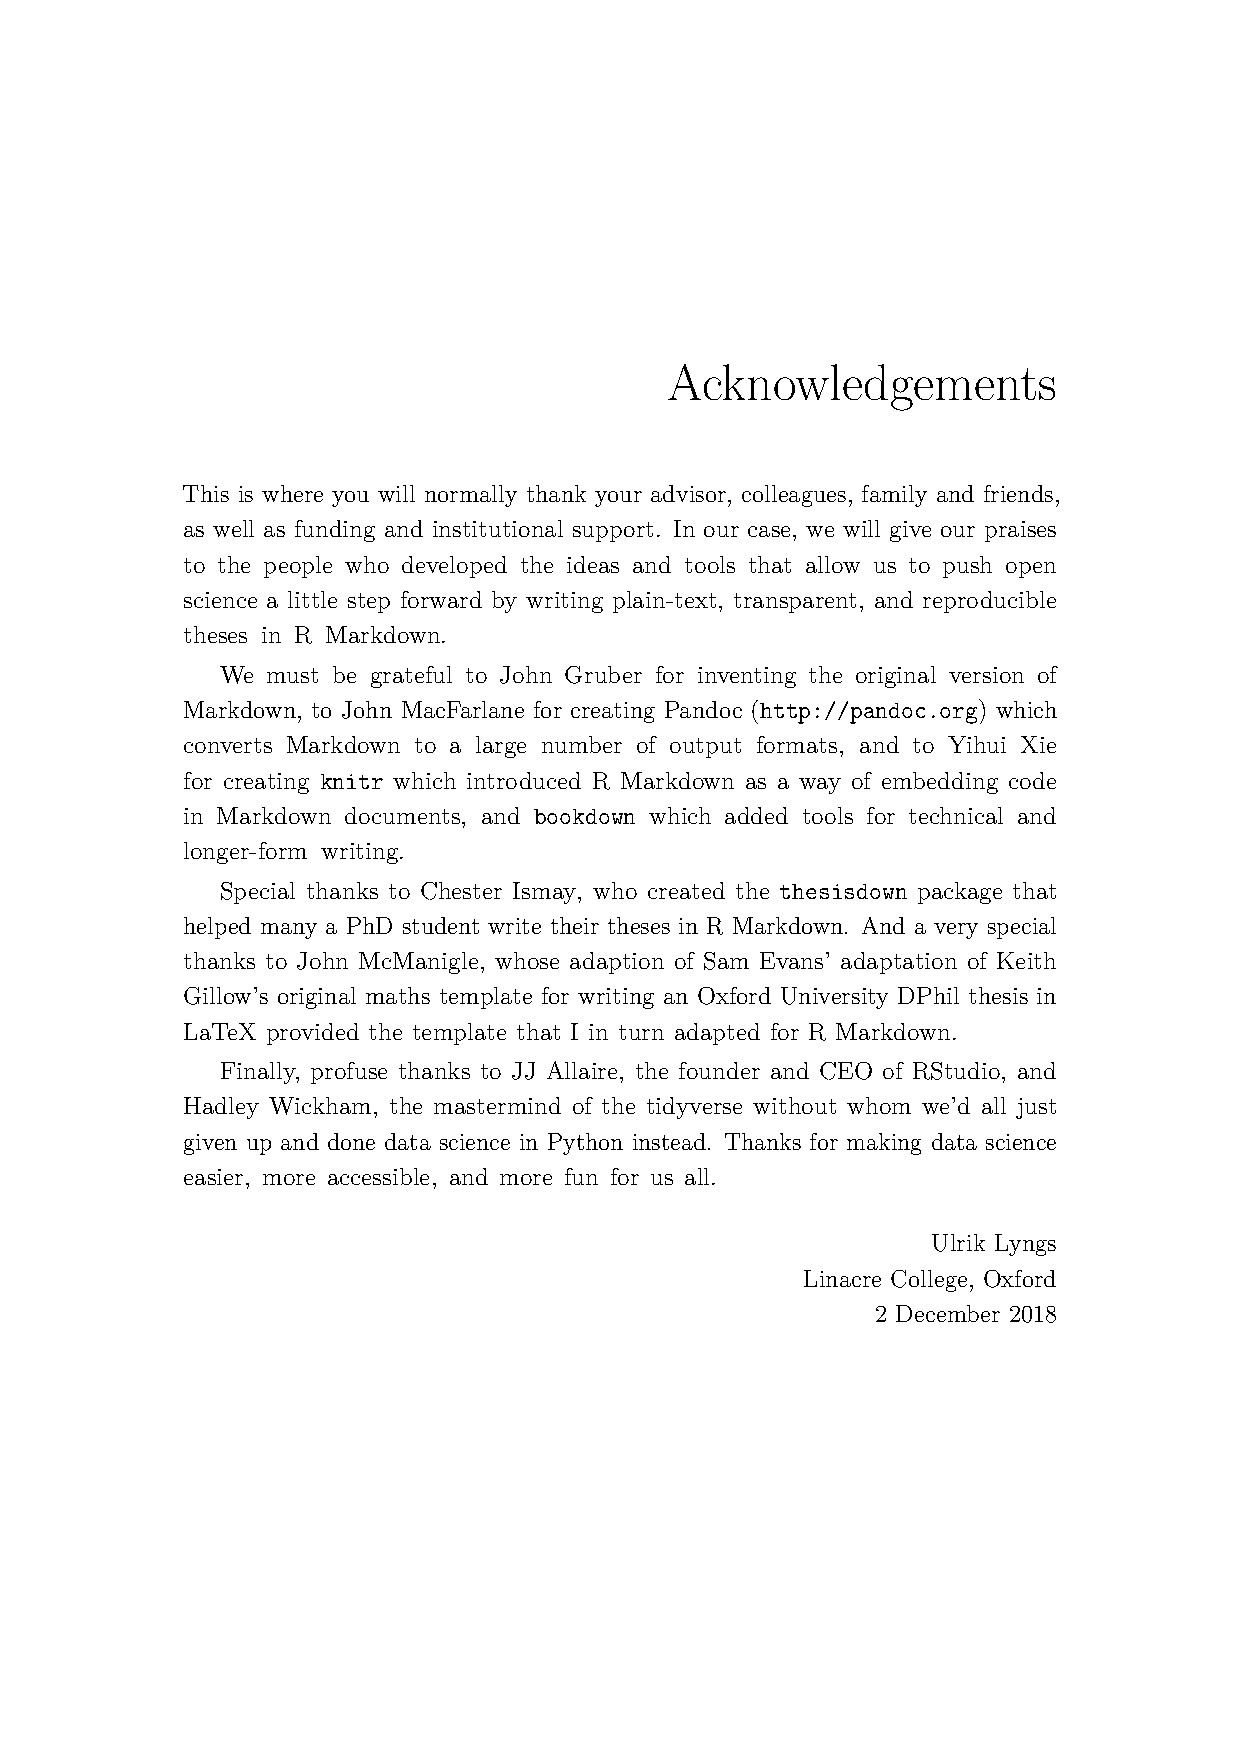
\includegraphics[width=0.32\linewidth]{figures/sample-content/alt_frontmatter_example/split/_000006.pdf}}

\hypertarget{risoluzione-dei-problemi}{%
\chapter{Risoluzione dei problemi}\label{risoluzione-dei-problemi}}

Questo capitolo descrive gli errori comuni che potresti incontrare e come risolverli.

\hypertarget{errore-impossibile-creare-la-bibliografia-tramite-biber}{%
\section{Errore: impossibile creare la bibliografia tramite biber}\label{errore-impossibile-creare-la-bibliografia-tramite-biber}}

Questo può accadere se hai avuto una build non riuscita, forse in relazione all'arresto improvviso di RStudio.

Prova a fare questo:

\begin{enumerate}
\def\labelenumi{\arabic{enumi}.}
\tightlist
\item
  digita \texttt{make\ clean-knits} nella scheda del terminale (o esegui \texttt{file.remove(list.files(pattern\ =\ "*.(log\textbar{}mtc\textbar{}maf\textbar{}aux\textbar{}bbl\textbar{}blg\textbar{}xml)"))} in la console R) per ripulire i file generati da LaTeX durante una build
\item
  riavvia il computer
\end{enumerate}

Se ciò non risolve il problema, prova a utilizzare il pacchetto LaTeX \href{https://www.overleaf.com/learn/latex/Bibliography_management_with_natbib}{natbib} invece di \href{https://www.overleaf.com/learn\%20/latex/Articles/Getting_started_with_BibLaTeX}{biblatex} per la gestione dei riferimenti.
Per fare ciò, vai su \textbf{index.Rmd} e

\begin{enumerate}
\def\labelenumi{\arabic{enumi}.}
\tightlist
\item
  imposta \texttt{use-bilatex:\ false} e \hspace{0pt}\hspace{0pt}\texttt{use-natbib:\ true}
\item
  imposta \texttt{citation\_package:\ natbib} sotto
\end{enumerate}

\begin{Shaded}
\begin{Highlighting}[]
\FunctionTok{output}\KeywordTok{:}
\AttributeTok{  bookdown:}\FunctionTok{:pdf\_book}\KeywordTok{:}
\AttributeTok{    }\FunctionTok{citation\_package}\KeywordTok{:}\AttributeTok{ natbib}
\end{Highlighting}
\end{Shaded}

\begin{savequote}
Alles Gescheite ist schon gedacht worden.\\
Man muss nur versuchen, es noch einmal zu denken.

All intelligent thoughts have already been thought;\\
what is necessary is only to try to think them again.
\qauthor{--- Johann Wolfgang von Goethe (\protect\hyperlink{ref-von_goethe_wilhelm_1829}{Goethe, 1829})}\end{savequote}



\hypertarget{conclusioni}{%
\chapter*{Conclusioni}\label{conclusioni}}
\addcontentsline{toc}{chapter}{Conclusioni}

Se non vogliamo che ``Conclusioni'' abbia un numero di capitolo accanto, possiamo aggiungere l'attributo \texttt{\{-\}}.

\hypertarget{ulteriori-informazioni}{%
\section*{Ulteriori informazioni}\label{ulteriori-informazioni}}
\addcontentsline{toc}{section}{Ulteriori informazioni}

Ed ecco alcune altre informazioni casuali:
il primo paragrafo dopo il titolo di un capitolo o l'intestazione di una sezione \emph{non dovrebbe essere} rientrato, perché i rientri devono dire al lettore che stai iniziando un nuovo paragrafo.

Questo paragrafo, al contrario, \emph{sarà} rientrato come dovrebbe perché non è il primo dopo il titolo ``Maggiori informazioni''.
Ciao LaTeX. (Se stai leggendo la versione HTML, non vedrai alcun rientro - dai un'occhiata alla versione PDF per capire di cosa diavolo sta parlando questa sezione).

\startappendices

\hypertarget{prima-appendice}{%
\chapter{Prima Appendice}\label{prima-appendice}}

Questa prima appendice include un pezzo R nascosto nel documento (usando l'opzione chunk \texttt{echo\ =\ FALSE}) per facilitare la leggibilità:

\textbf{In 02-rmd-basics-code.Rmd}

\begin{Shaded}
\begin{Highlighting}[]
\FunctionTok{library}\NormalTok{(tidyverse)}
\NormalTok{knitr}\SpecialCharTok{::}\FunctionTok{include\_graphics}\NormalTok{(}\StringTok{"figures/sample{-}content/chunk{-}parts.png"}\NormalTok{)}
\end{Highlighting}
\end{Shaded}

\textbf{And here's another one from the same chapter, i.e.~Chapter \ref{code}:}

\hypertarget{la-seconda-appendice-per-ischerzo}{%
\chapter{la Seconda Appendice, per ischerzo}\label{la-seconda-appendice-per-ischerzo}}

\hypertarget{references}{%
\chapter*{References}\label{references}}
\addcontentsline{toc}{chapter}{References}

\hypertarget{refs}{}
\begin{CSLReferences}{1}{0}
\leavevmode\vadjust pre{\hypertarget{ref-Darwin1859}{}}%
Darwin, C. (1859). \emph{{On the Origin of Species by Means of Natural Selection or the Preservation of Favoured Races in the Struggle for Life}}. John Murray.

\leavevmode\vadjust pre{\hypertarget{ref-von_goethe_wilhelm_1829}{}}%
Goethe, J. W. von. (1829). \emph{Wilhelm {Meisters} {Wanderjahre} oder die {Entsagenden}}. Cotta.

\leavevmode\vadjust pre{\hypertarget{ref-Lottridge2012}{}}%
Lottridge, D., Marschner, E., Wang, E., Romanovsky, M., \& Nass, C. (2012). {Browser design impacts multitasking}. \emph{Proceedings of the Human Factors and Ergonomics Society 56th Annual Meeting}. \url{https://doi.org/10.1177/1071181312561289}

\leavevmode\vadjust pre{\hypertarget{ref-Mill1965}{}}%
Mill, J. S. (1965 {[}1843{]}). \emph{A system of logic, ratiocinative and inductive: Being a connected view of the principles of evidence and the methods of scientific investigation}. Longmans.

\leavevmode\vadjust pre{\hypertarget{ref-Shea2014}{}}%
Shea, N., Boldt, A., Bang, D., Yeung, N., Heyes, C., \& Frith, C. D. (2014). {Supra-personal cognitive control and metacognition}. \emph{Trends in Cognitive Sciences}, \emph{18}(4), 186--193. \url{https://doi.org/10.1016/j.tics.2014.01.006}

\leavevmode\vadjust pre{\hypertarget{ref-Wu2016}{}}%
Wu, T. (2016). \emph{{The Attention Merchants: The Epic Scramble to Get Inside Our Heads}}. Knopf Publishing Group.

\end{CSLReferences}

%%%%% REFERENCES


\end{document}
